% Options for packages loaded elsewhere
\PassOptionsToPackage{unicode}{hyperref}
\PassOptionsToPackage{hyphens}{url}
%
\documentclass[
]{article}
\usepackage{amsmath,amssymb}
\usepackage{iftex}
\ifPDFTeX
  \usepackage[T1]{fontenc}
  \usepackage[utf8]{inputenc}
  \usepackage{textcomp} % provide euro and other symbols
\else % if luatex or xetex
  \usepackage{unicode-math} % this also loads fontspec
  \defaultfontfeatures{Scale=MatchLowercase}
  \defaultfontfeatures[\rmfamily]{Ligatures=TeX,Scale=1}
\fi
\usepackage{lmodern}
\ifPDFTeX\else
  % xetex/luatex font selection
\fi
% Use upquote if available, for straight quotes in verbatim environments
\IfFileExists{upquote.sty}{\usepackage{upquote}}{}
\IfFileExists{microtype.sty}{% use microtype if available
  \usepackage[]{microtype}
  \UseMicrotypeSet[protrusion]{basicmath} % disable protrusion for tt fonts
}{}
\makeatletter
\@ifundefined{KOMAClassName}{% if non-KOMA class
  \IfFileExists{parskip.sty}{%
    \usepackage{parskip}
  }{% else
    \setlength{\parindent}{0pt}
    \setlength{\parskip}{6pt plus 2pt minus 1pt}}
}{% if KOMA class
  \KOMAoptions{parskip=half}}
\makeatother
\usepackage{xcolor}
\usepackage[margin=1in]{geometry}
\usepackage{graphicx}
\makeatletter
\newsavebox\pandoc@box
\newcommand*\pandocbounded[1]{% scales image to fit in text height/width
  \sbox\pandoc@box{#1}%
  \Gscale@div\@tempa{\textheight}{\dimexpr\ht\pandoc@box+\dp\pandoc@box\relax}%
  \Gscale@div\@tempb{\linewidth}{\wd\pandoc@box}%
  \ifdim\@tempb\p@<\@tempa\p@\let\@tempa\@tempb\fi% select the smaller of both
  \ifdim\@tempa\p@<\p@\scalebox{\@tempa}{\usebox\pandoc@box}%
  \else\usebox{\pandoc@box}%
  \fi%
}
% Set default figure placement to htbp
\def\fps@figure{htbp}
\makeatother
\setlength{\emergencystretch}{3em} % prevent overfull lines
\providecommand{\tightlist}{%
  \setlength{\itemsep}{0pt}\setlength{\parskip}{0pt}}
\setcounter{secnumdepth}{-\maxdimen} % remove section numbering
\ifLuaTeX
\usepackage[bidi=basic]{babel}
\else
\usepackage[bidi=default]{babel}
\fi
\babelprovide[main,import]{french}
% get rid of language-specific shorthands (see #6817):
\let\LanguageShortHands\languageshorthands
\def\languageshorthands#1{}
\usepackage{bookmark}
\IfFileExists{xurl.sty}{\usepackage{xurl}}{} % add URL line breaks if available
\urlstyle{same}
\hypersetup{
  pdftitle={Synthèse des comptes trimestriels : approche offre et demande},
  pdfauthor={@statjunior},
  pdflang={fr-FR},
  hidelinks,
  pdfcreator={LaTeX via pandoc}}

\title{Synthèse des comptes trimestriels : approche offre et demande}
\usepackage{etoolbox}
\makeatletter
\providecommand{\subtitle}[1]{% add subtitle to \maketitle
  \apptocmd{\@title}{\par {\large #1 \par}}{}{}
}
\makeatother
\subtitle{Résultats provisoires des \emph{Comptes Nationaux
Trimestriels} au 2e trimestre 2024.}
\author{@statjunior}
\date{30 juillet 2024}

\begin{document}
\maketitle

\section{Présentation}\label{pruxe9sentation}

Ce rapport \emph{RMarkdown} présente les résultats provisoires des
comptes de branche au 2e trimestre 2024. On présente les grands agrégats
économiques de la production (PIB) et divers indicateurs relatifs à la
production (productivité du travail, salaire moyen par tête, taux de
marge \ldots).

Dans un premier temps, on s'intéresse à la croissance trimestrielle du
PIB. On constate les contributions à l'évolution du PIB par composante
de la demande (Consommation, Investissement, Solde extérieur, Variations
de stocks). On compare le PIB en variation trimestrielle et en évolution
depuis la Crise du Covid.

On présente également l'évolution du solde extérieur de la France
(exports - imports).

Un focus analyse l'évolution de la consommation des ménages depuis le
Covid, en particulier pour la consommation alimentaire et énergétique.

On se penche ensuite sur la conjoncture économique des secteurs
d'activité de l'économie française. On présente les gains (ou les
pertes) de valeur ajoutée par branche depuis le Covid.

Une attention particulière est portée à l'évolution de la productivité
du travail depuis la crise du Covid. En lien avec la productivité du
travail, on constate l'évolution du Salaire Moyen par Tête.

Le rapport se conclut enfin par un développement détaillé des marges
sectorielles des entreprises. Une attention particulière est portée aux
secteurs énergétiques dont les profits ont considérablement augmenté
depuis 2021.

Ce rapport a été compilé automatiquement avec le logiciel \texttt{R}, le
30 juillet 2024 à 07 heures et 36 minutes. Les potentielles erreurs
présentes dans ce document relèvent uniquement de la responsabilité de
Statjunior.

Le code source permettant de générer ce document est disponible sur Git
\href{https://github.com/statjunior/Statjunior/tree/main/Conjoncture\%20-\%20comptes\%20trimestriels/}{en
cliquant ici}.

\newpage

\section{Croissance du PIB}\label{croissance-du-pib}

\subsection{Décomposition de la croissance du PIB trimestrielle par
l'approche demande (Conso+Investissement+(Export-Import)+Variations de
Stocks)}\label{duxe9composition-de-la-croissance-du-pib-trimestrielle-par-lapproche-demande-consoinvestissementexport-importvariations-de-stocks}

\pandocbounded{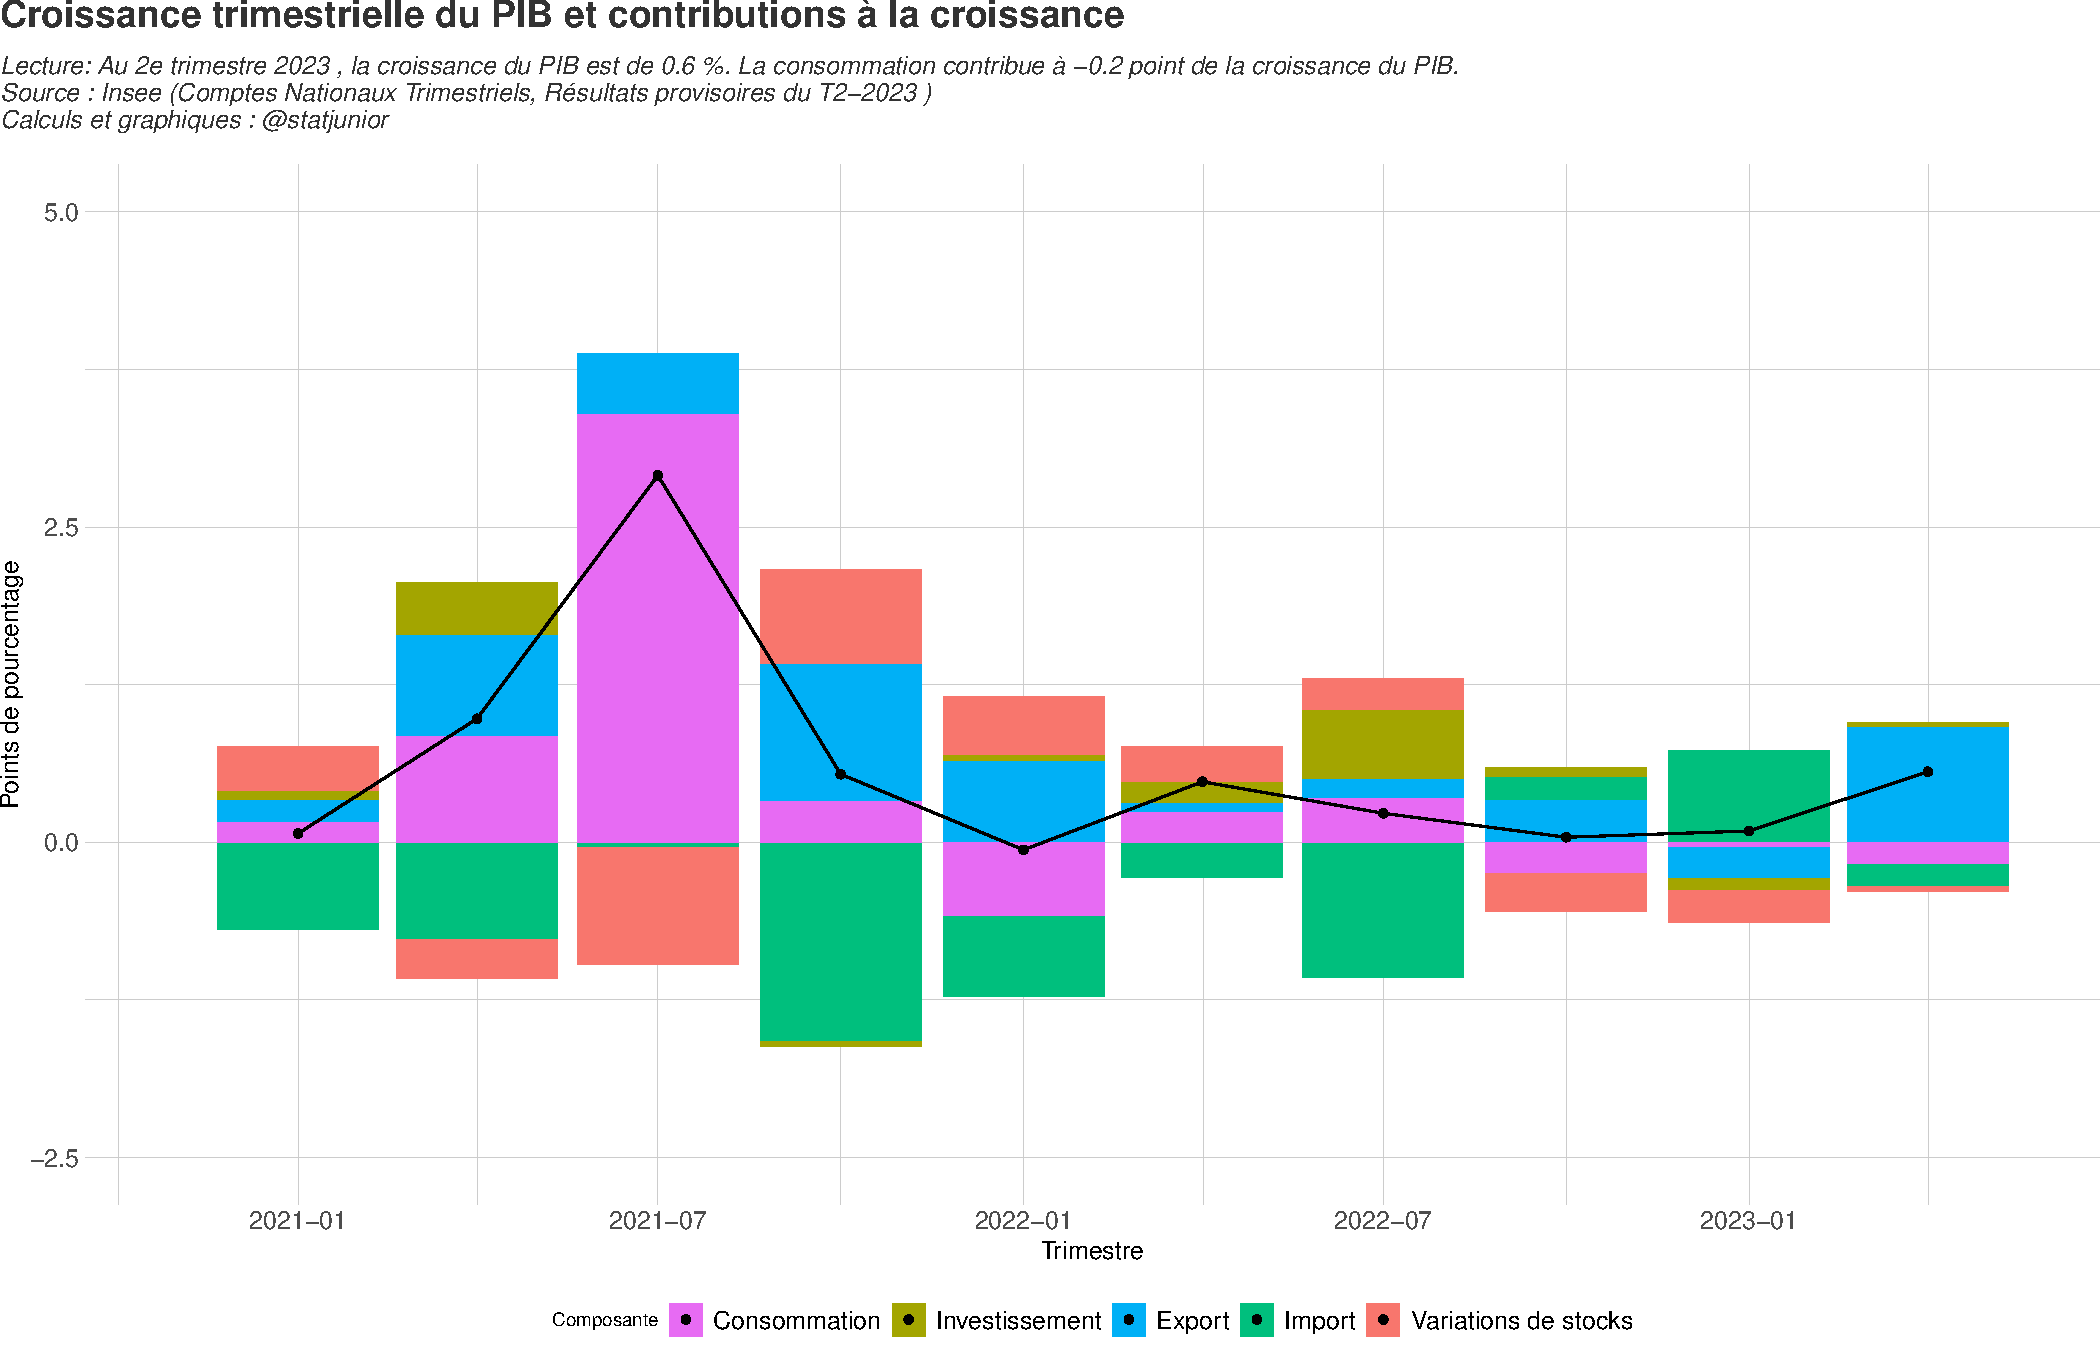
\includegraphics[keepaspectratio]{rapport_pdf_compte_branche_files/figure-latex/unnamed-chunk-2-1.pdf}}

\subsection{Evolution des composantes du PIB en volume par rapport au
T4-2019}\label{evolution-des-composantes-du-pib-en-volume-par-rapport-au-t4-2019}

\pandocbounded{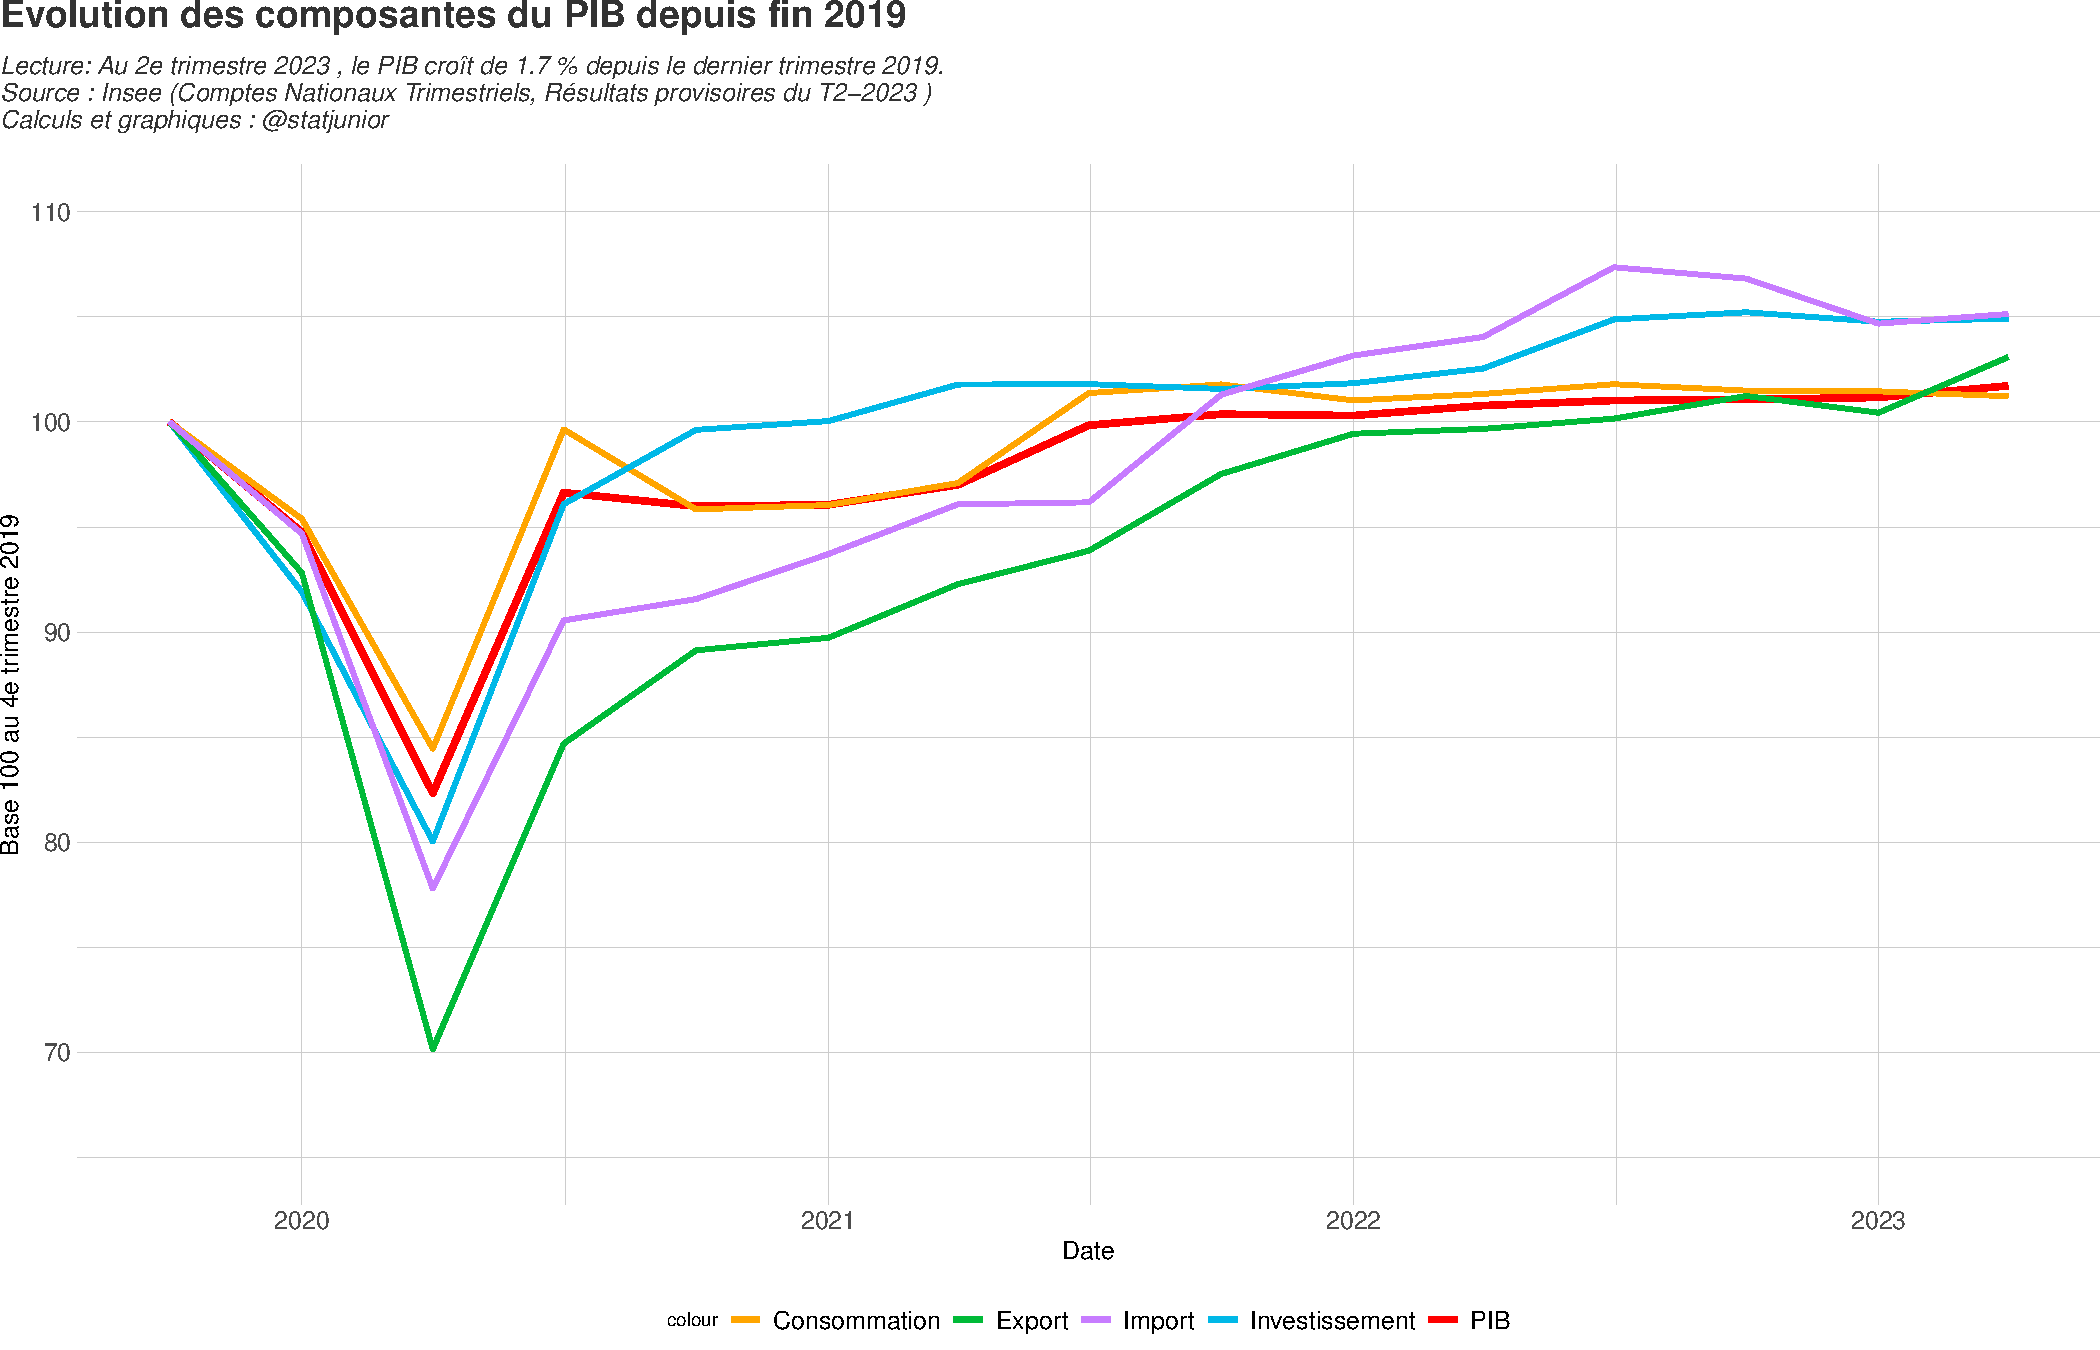
\includegraphics[keepaspectratio]{rapport_pdf_compte_branche_files/figure-latex/unnamed-chunk-3-1.pdf}}

\subsection{Evolution des composantes du PIB en volume par rapport au
T4-2021}\label{evolution-des-composantes-du-pib-en-volume-par-rapport-au-t4-2021}

\pandocbounded{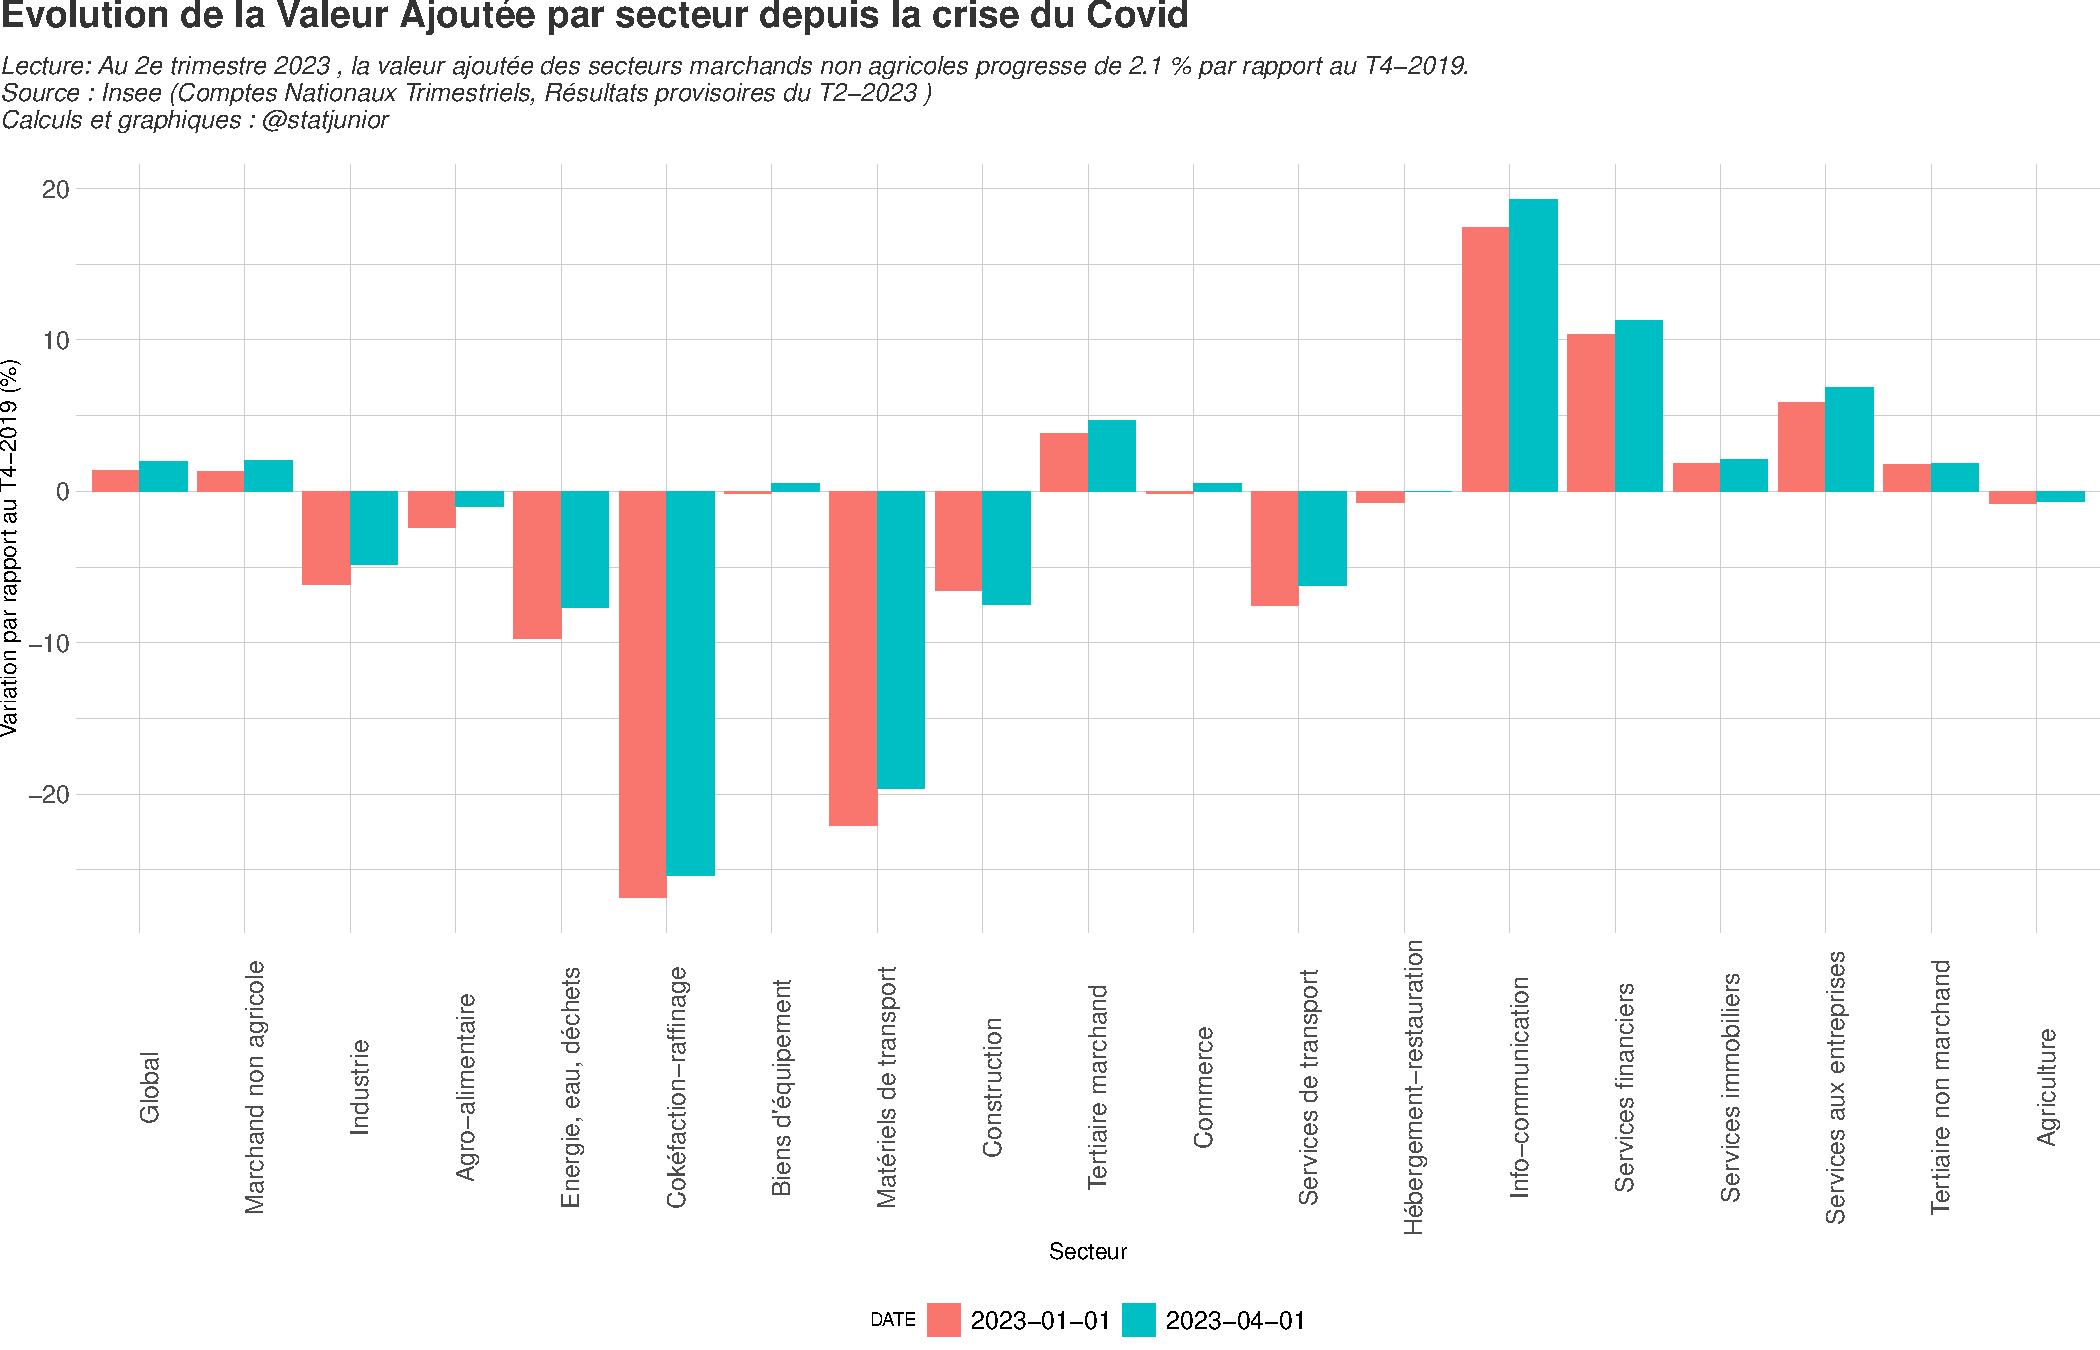
\includegraphics[keepaspectratio]{rapport_pdf_compte_branche_files/figure-latex/unnamed-chunk-4-1.pdf}}

\subsection{Evolution des composantes de la demande intérieure par
secteur institutionnel depuis le
T4-2021}\label{evolution-des-composantes-de-la-demande-intuxe9rieure-par-secteur-institutionnel-depuis-le-t4-2021}

\pandocbounded{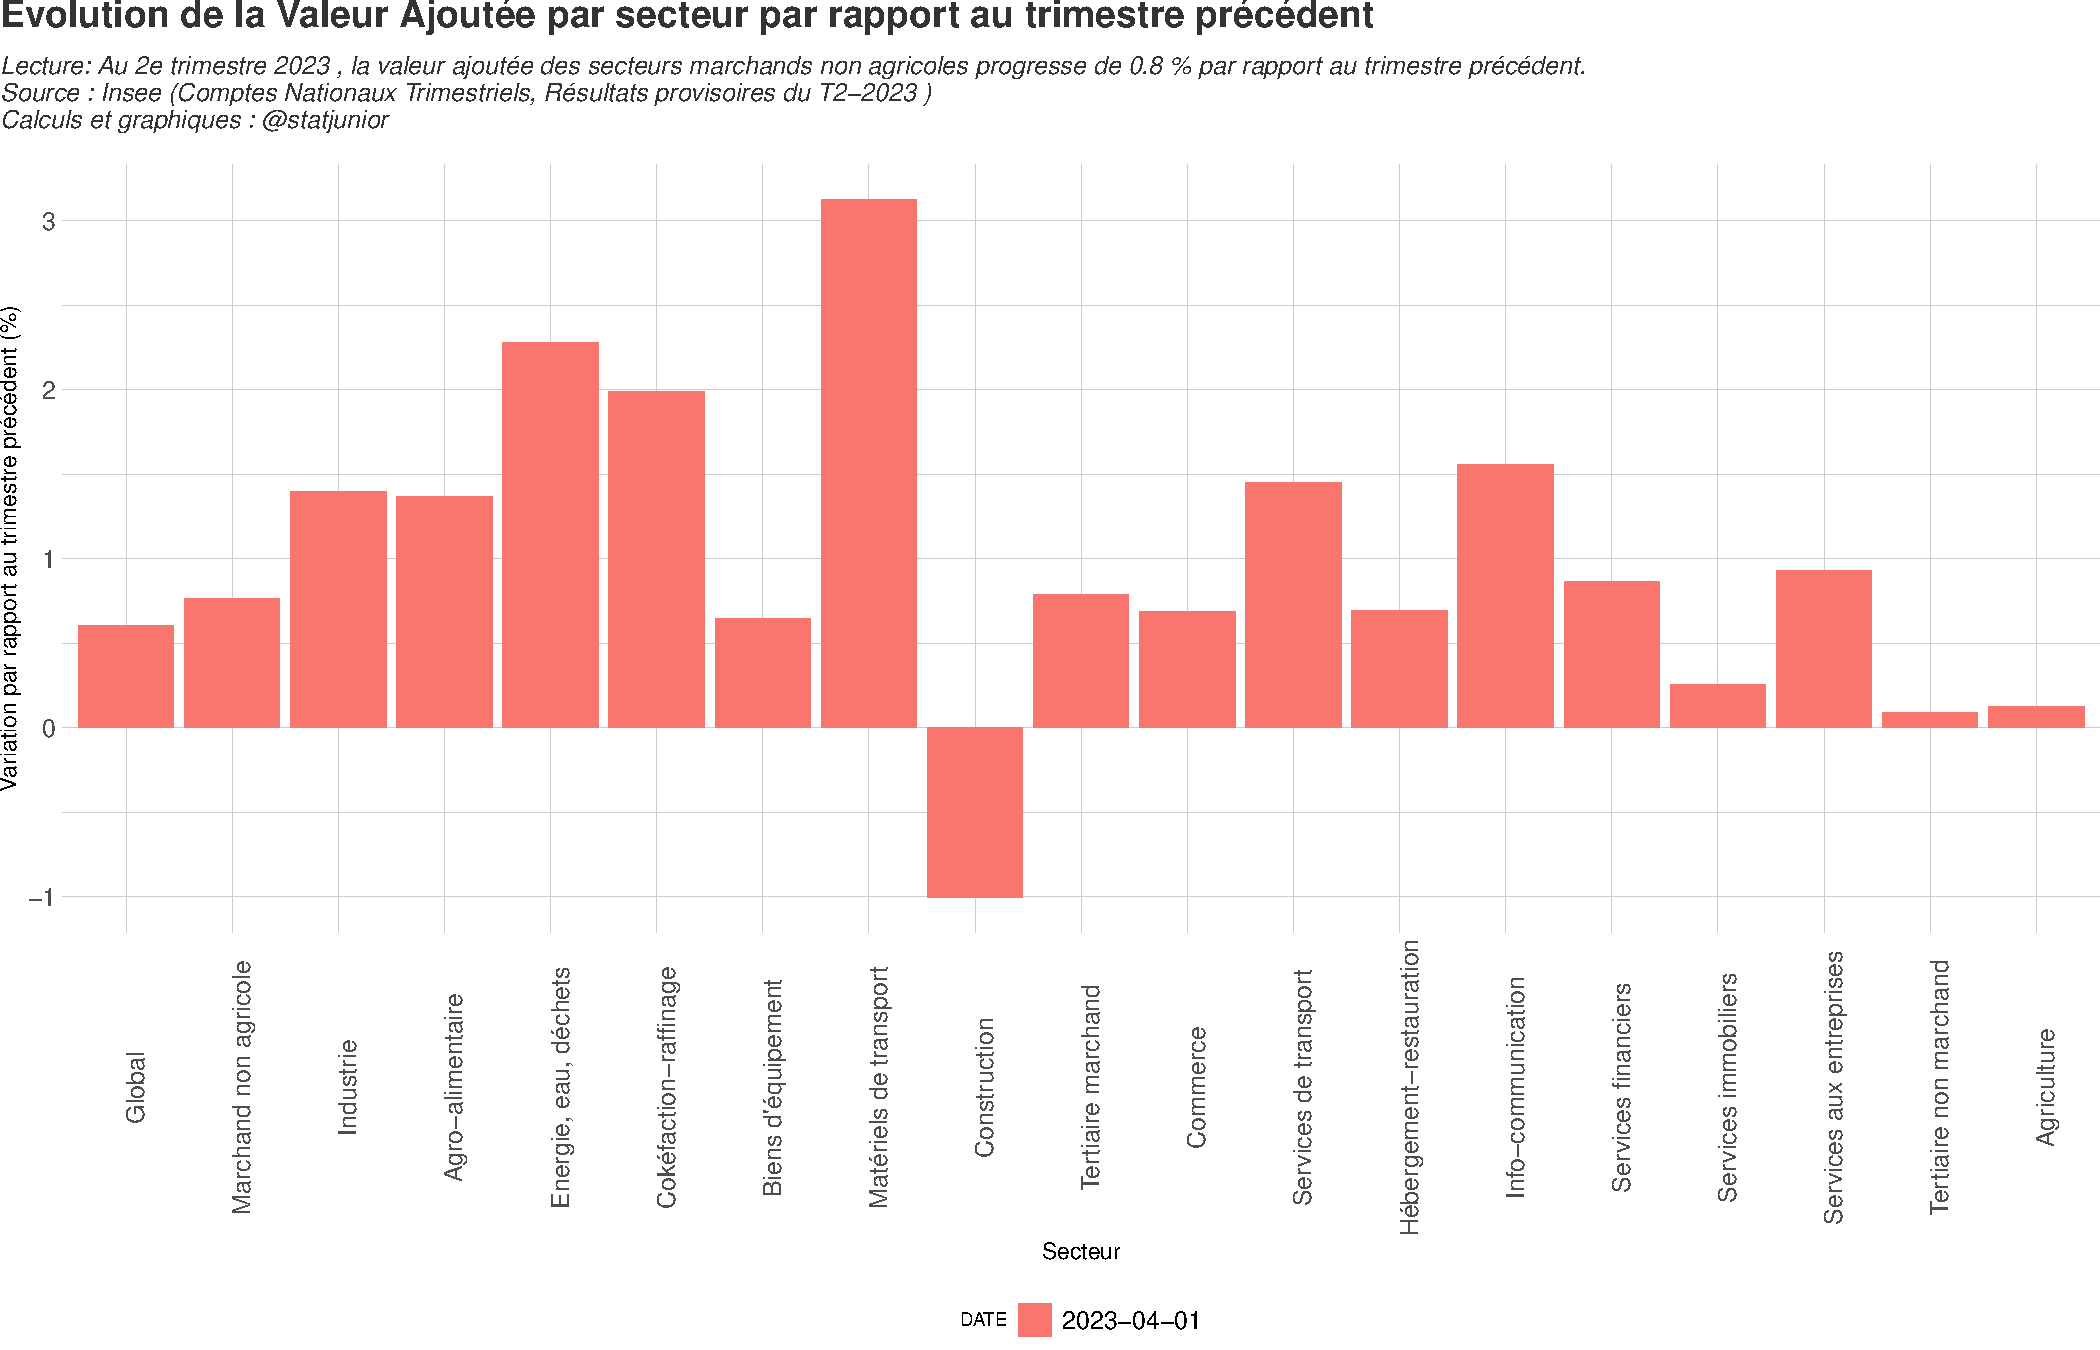
\includegraphics[keepaspectratio]{rapport_pdf_compte_branche_files/figure-latex/unnamed-chunk-5-1.pdf}}

\subsection{Valeur ajoutée par branche depuis fin
2019}\label{valeur-ajoutuxe9e-par-branche-depuis-fin-2019}

\pandocbounded{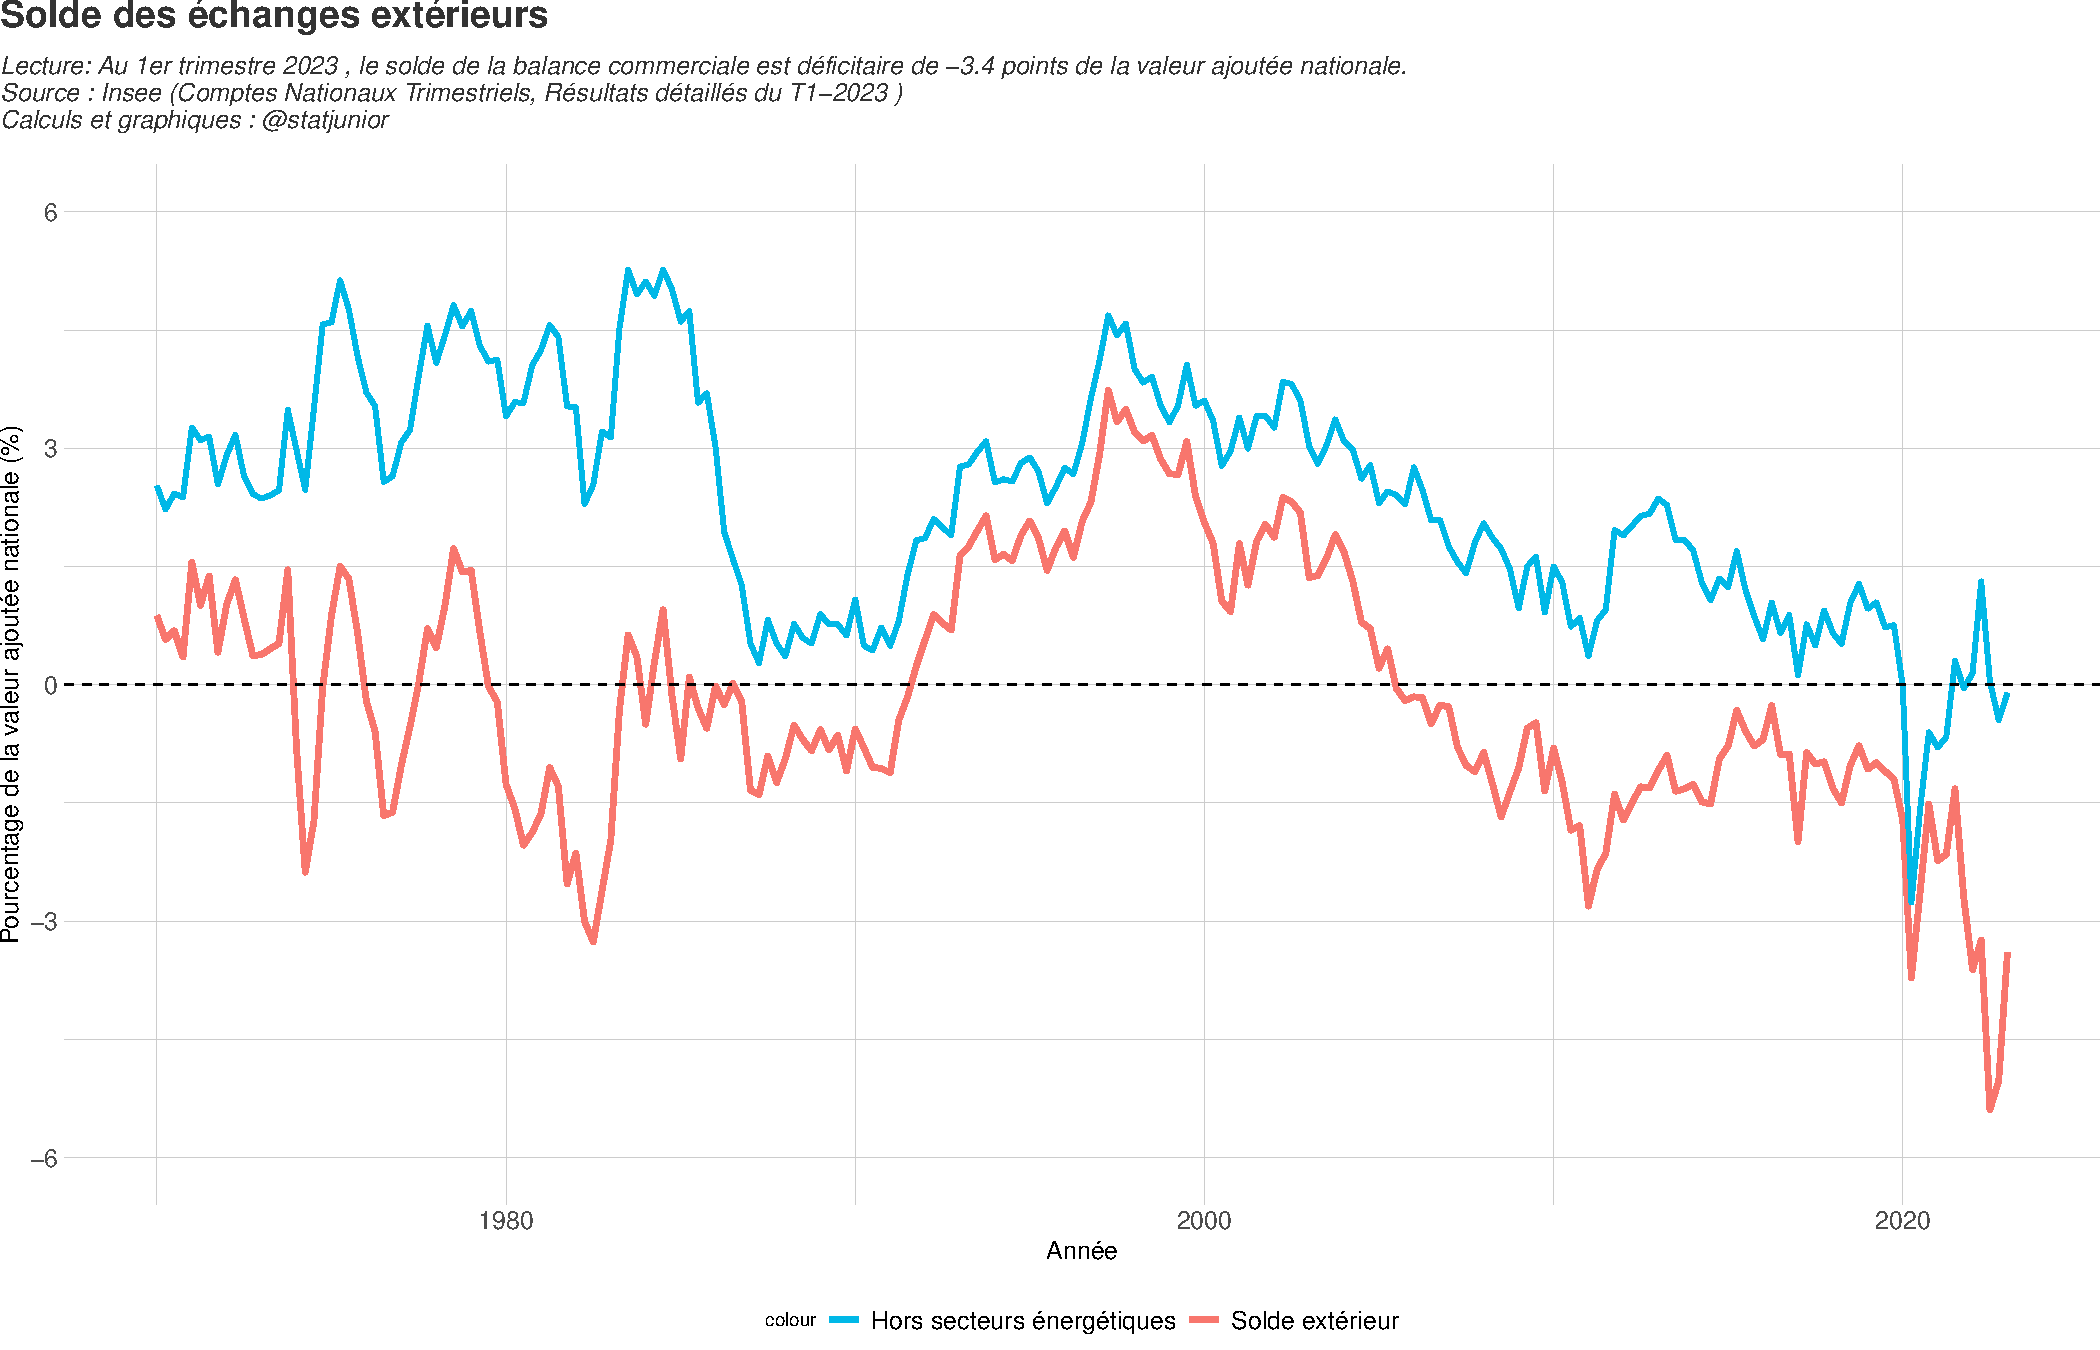
\includegraphics[keepaspectratio]{rapport_pdf_compte_branche_files/figure-latex/unnamed-chunk-6-1.pdf}}

\subsection{Valeur ajoutée par branche en glissement
annuel}\label{valeur-ajoutuxe9e-par-branche-en-glissement-annuel}

\pandocbounded{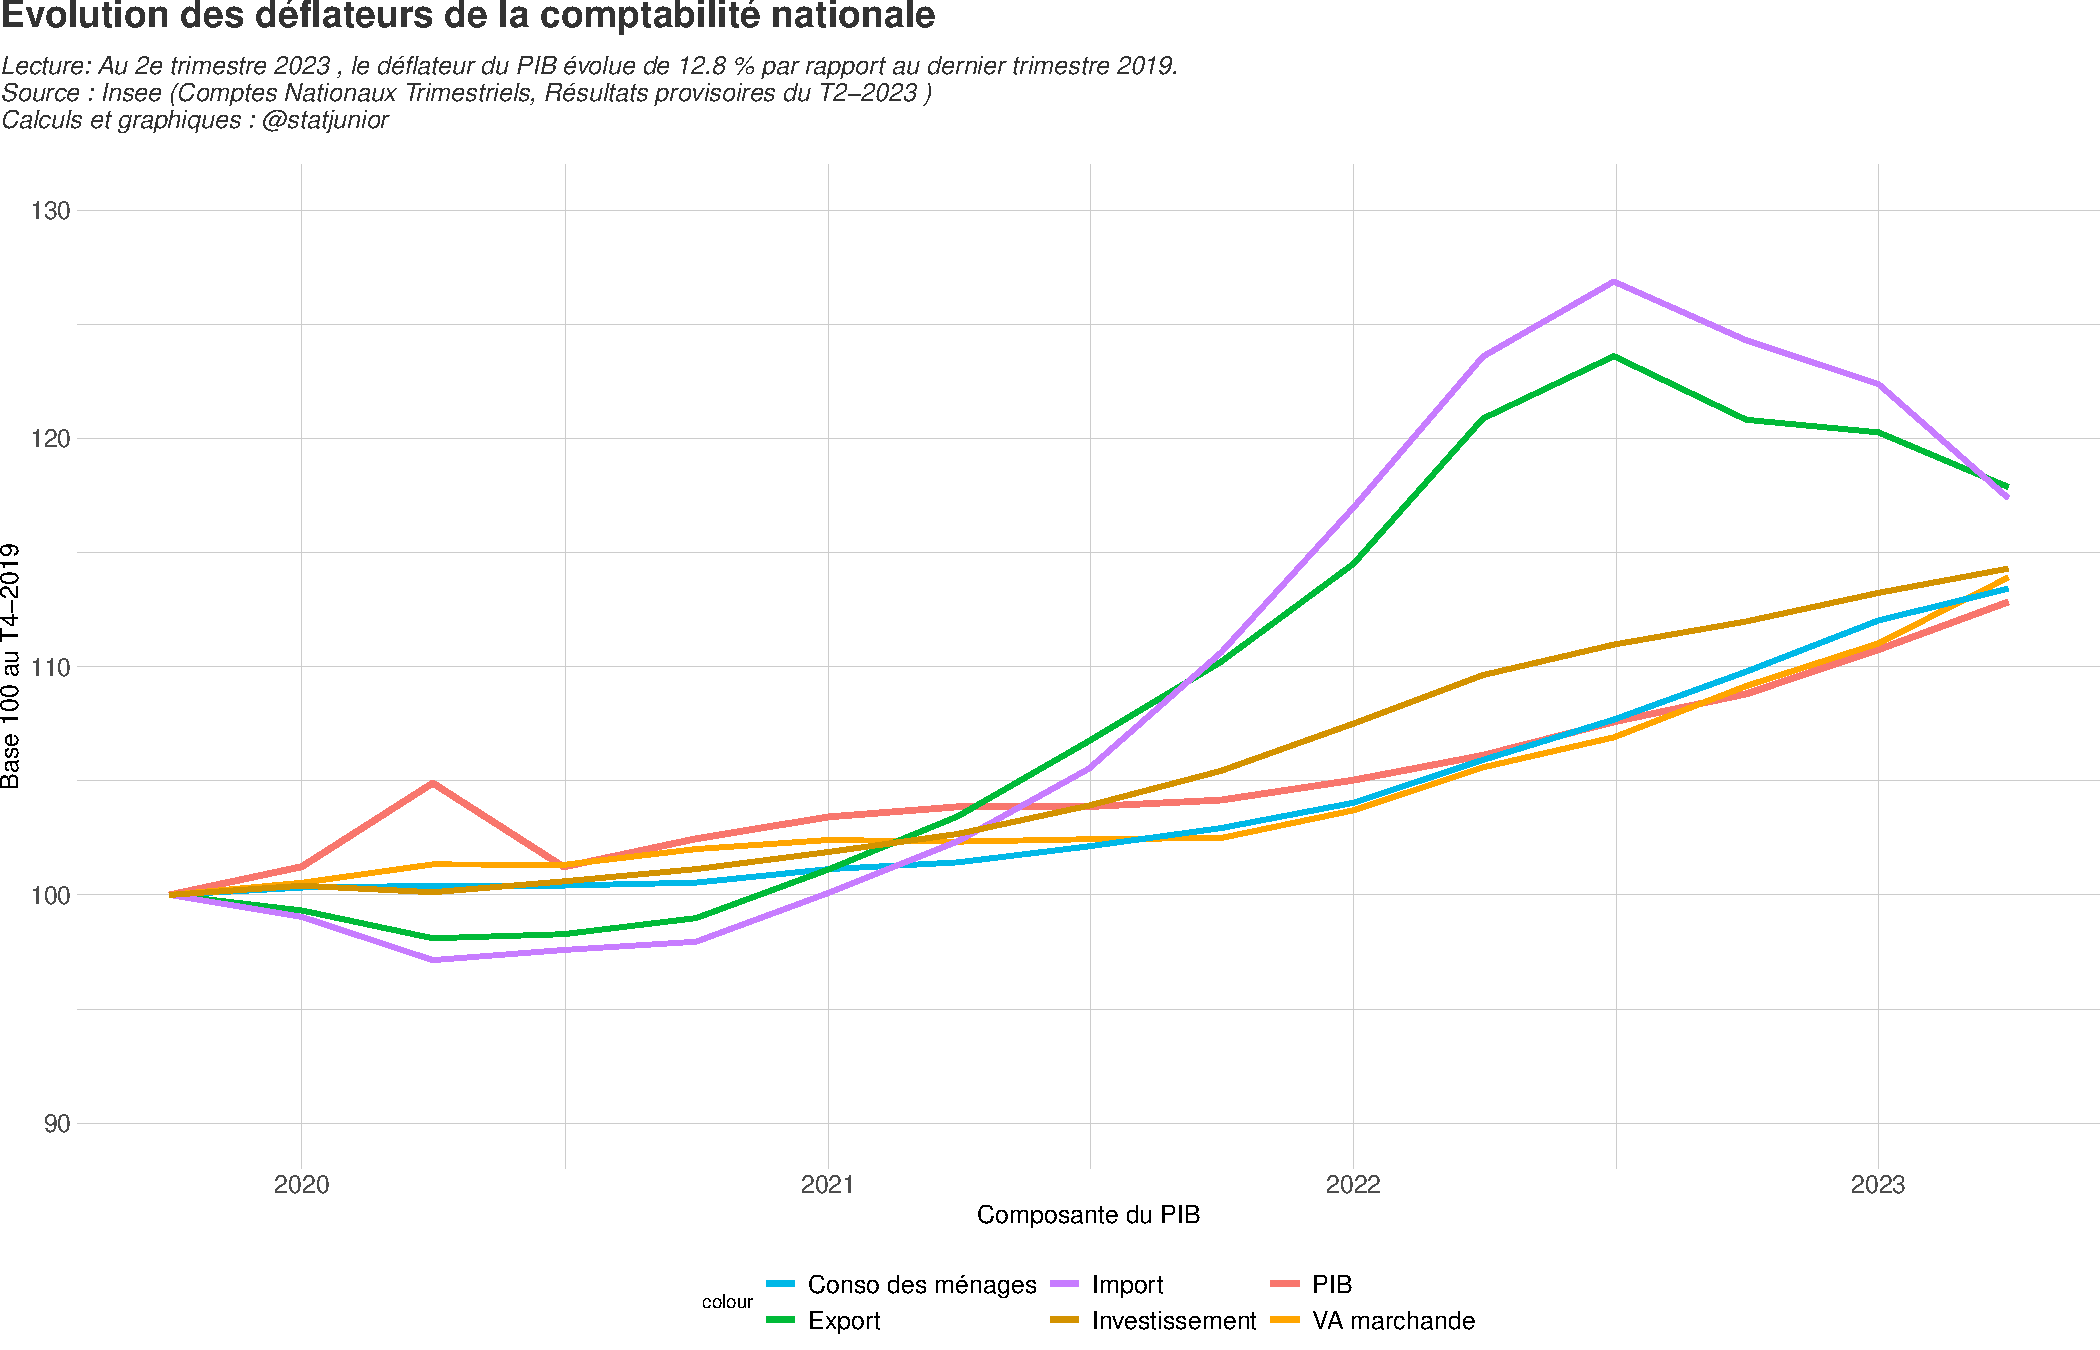
\includegraphics[keepaspectratio]{rapport_pdf_compte_branche_files/figure-latex/unnamed-chunk-7-1.pdf}}

\subsection{Progression de la valeur ajoutée par rapport au dernier
trimestre}\label{progression-de-la-valeur-ajoutuxe9e-par-rapport-au-dernier-trimestre}

\pandocbounded{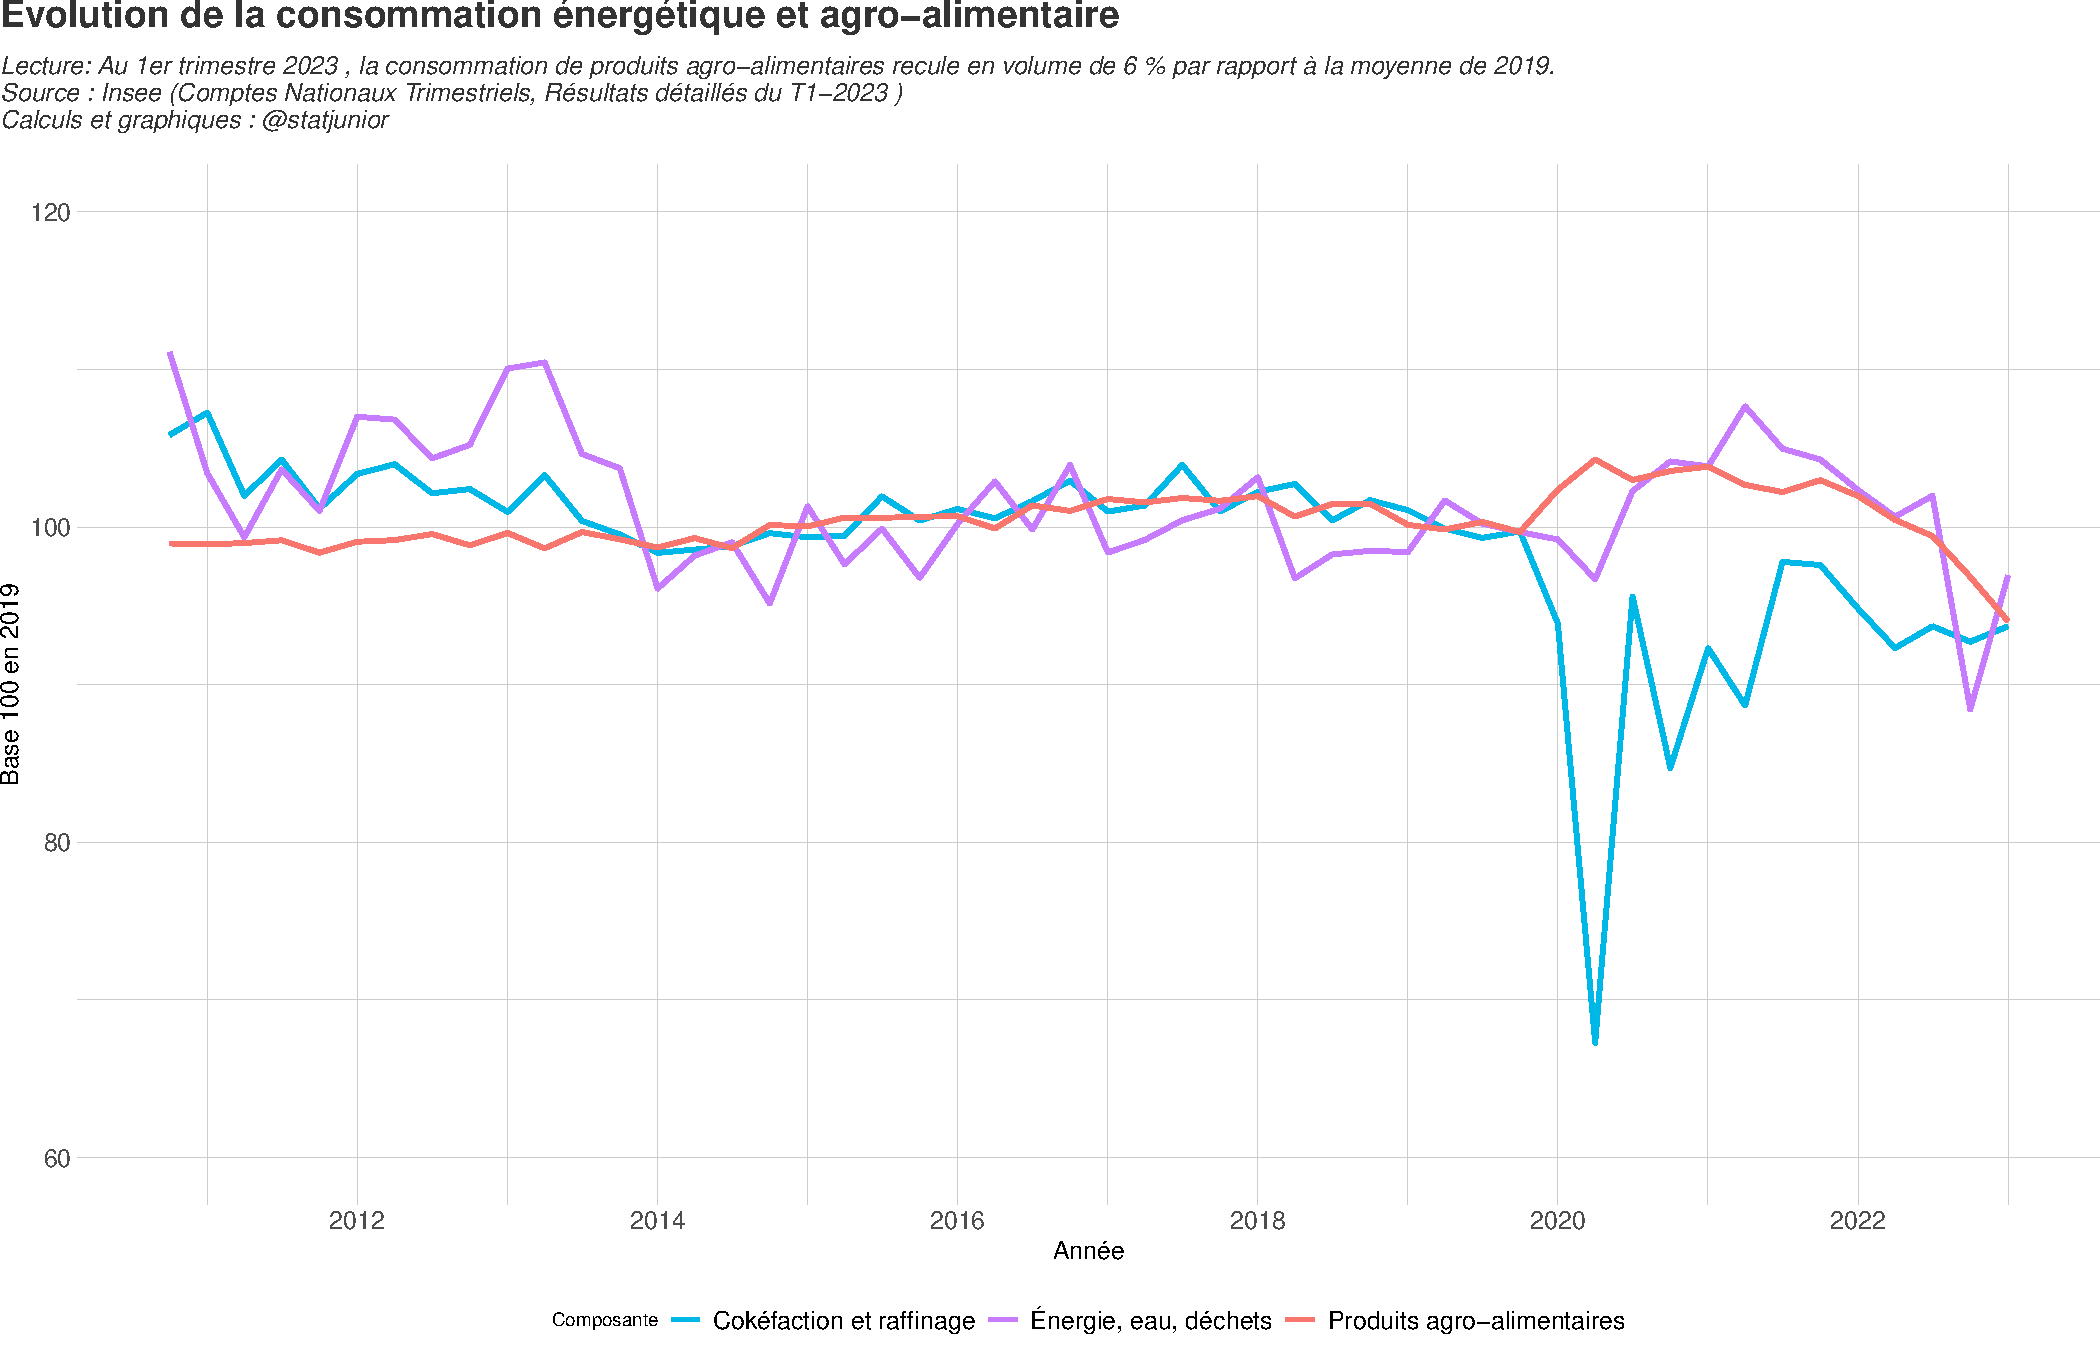
\includegraphics[keepaspectratio]{rapport_pdf_compte_branche_files/figure-latex/unnamed-chunk-8-1.pdf}}

\section{Evolution du prix des composantes du
PIB}\label{evolution-du-prix-des-composantes-du-pib}

\subsection{Inflation des composantes du PIB au dernier trimestre
connu}\label{inflation-des-composantes-du-pib-au-dernier-trimestre-connu}

\pandocbounded{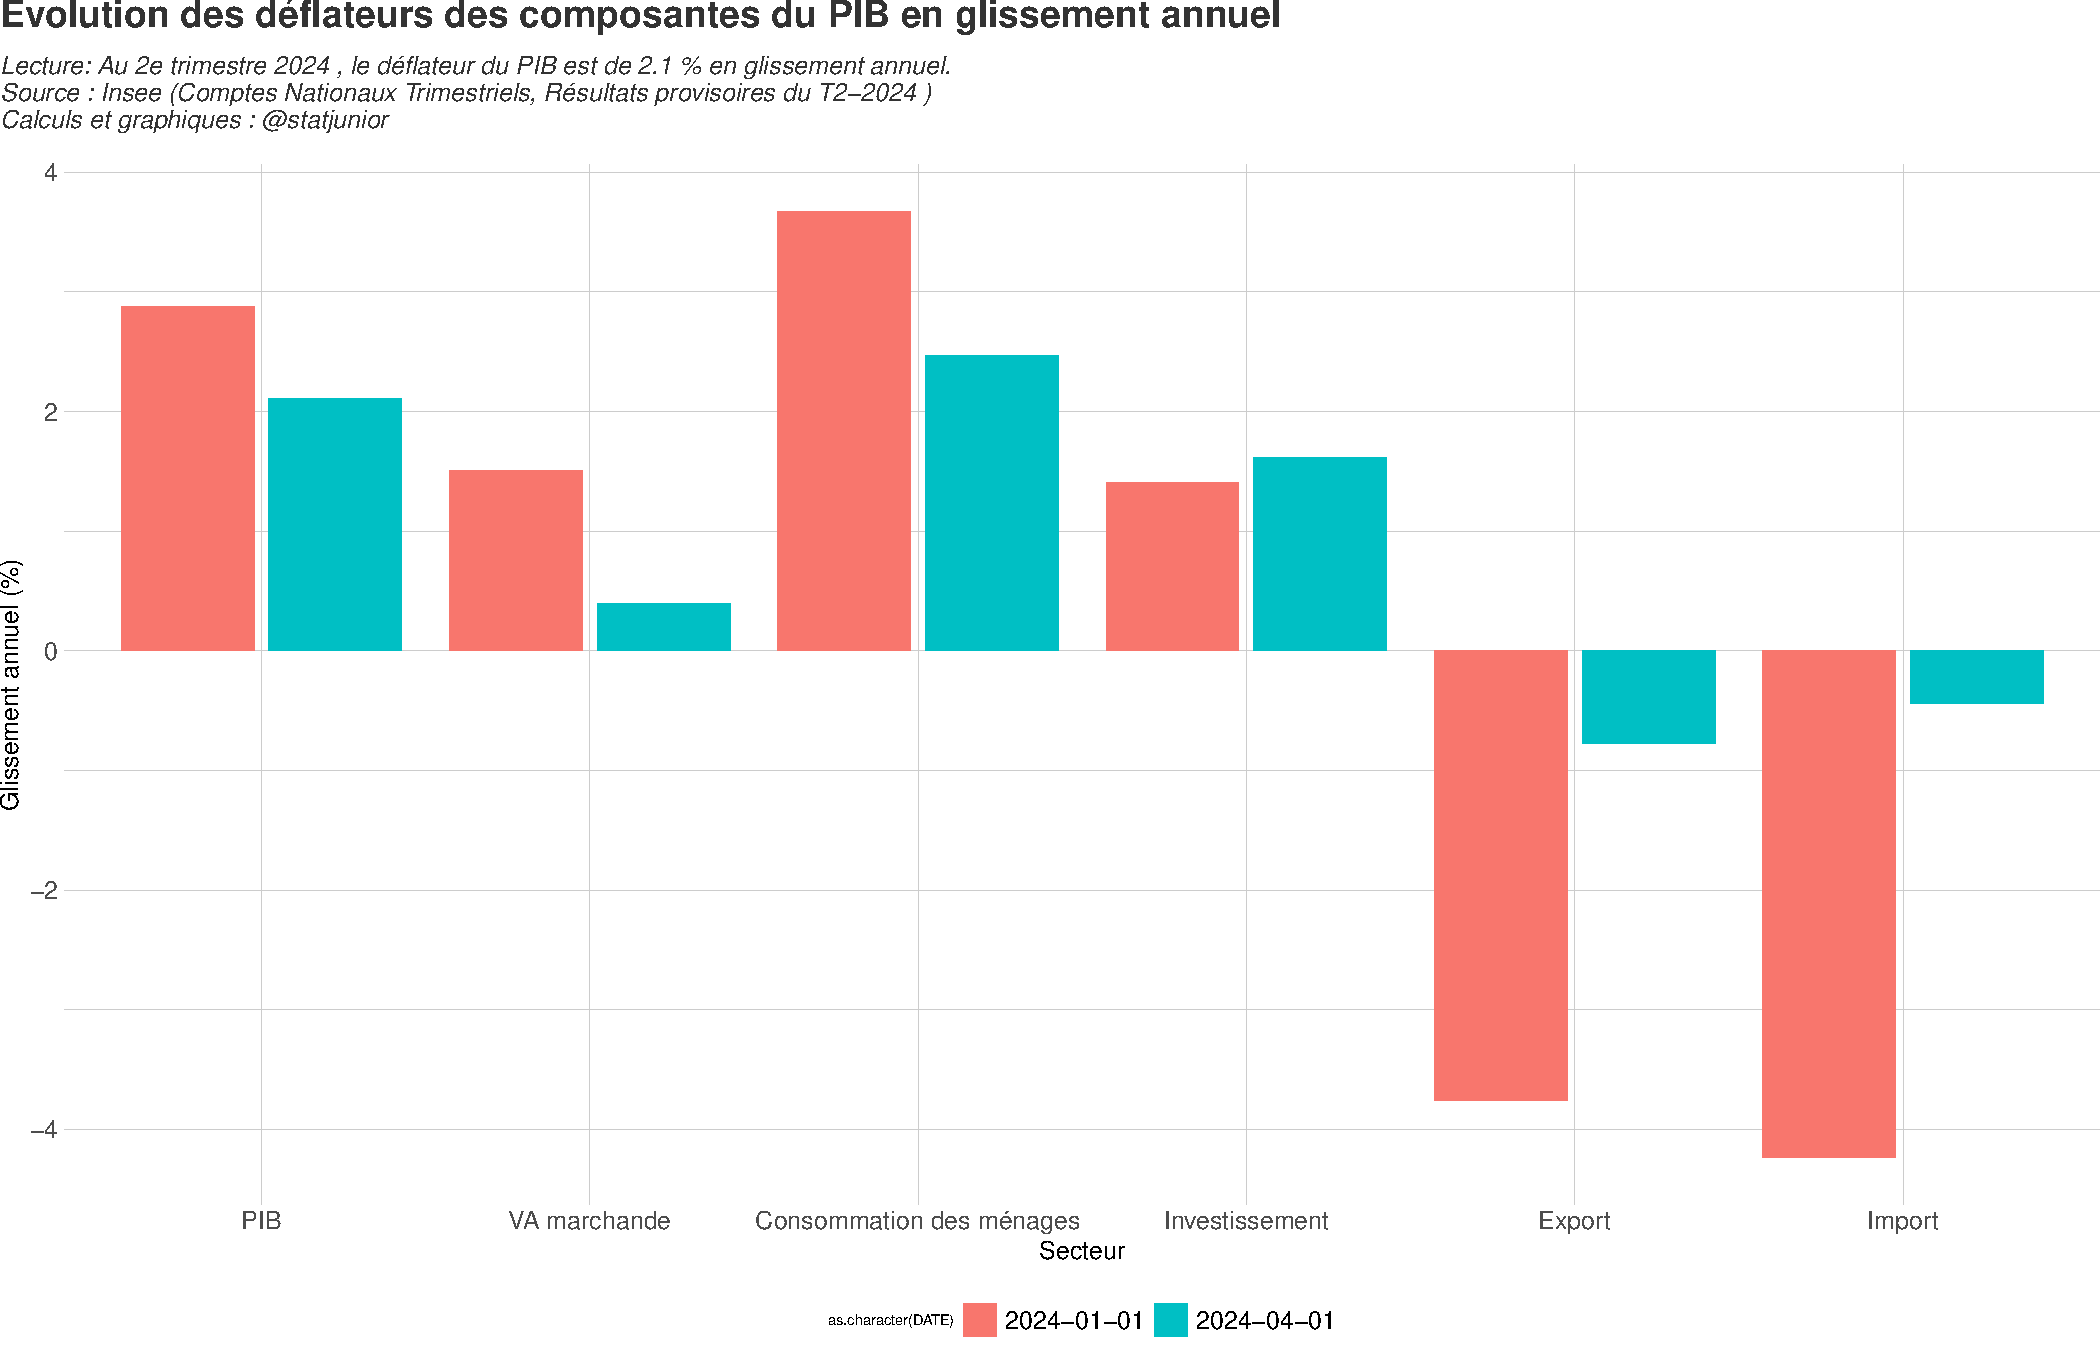
\includegraphics[keepaspectratio]{rapport_pdf_compte_branche_files/figure-latex/unnamed-chunk-9-1.pdf}}

\subsection{Prix des composantes du PIB depuis la fin
2019}\label{prix-des-composantes-du-pib-depuis-la-fin-2019}

\pandocbounded{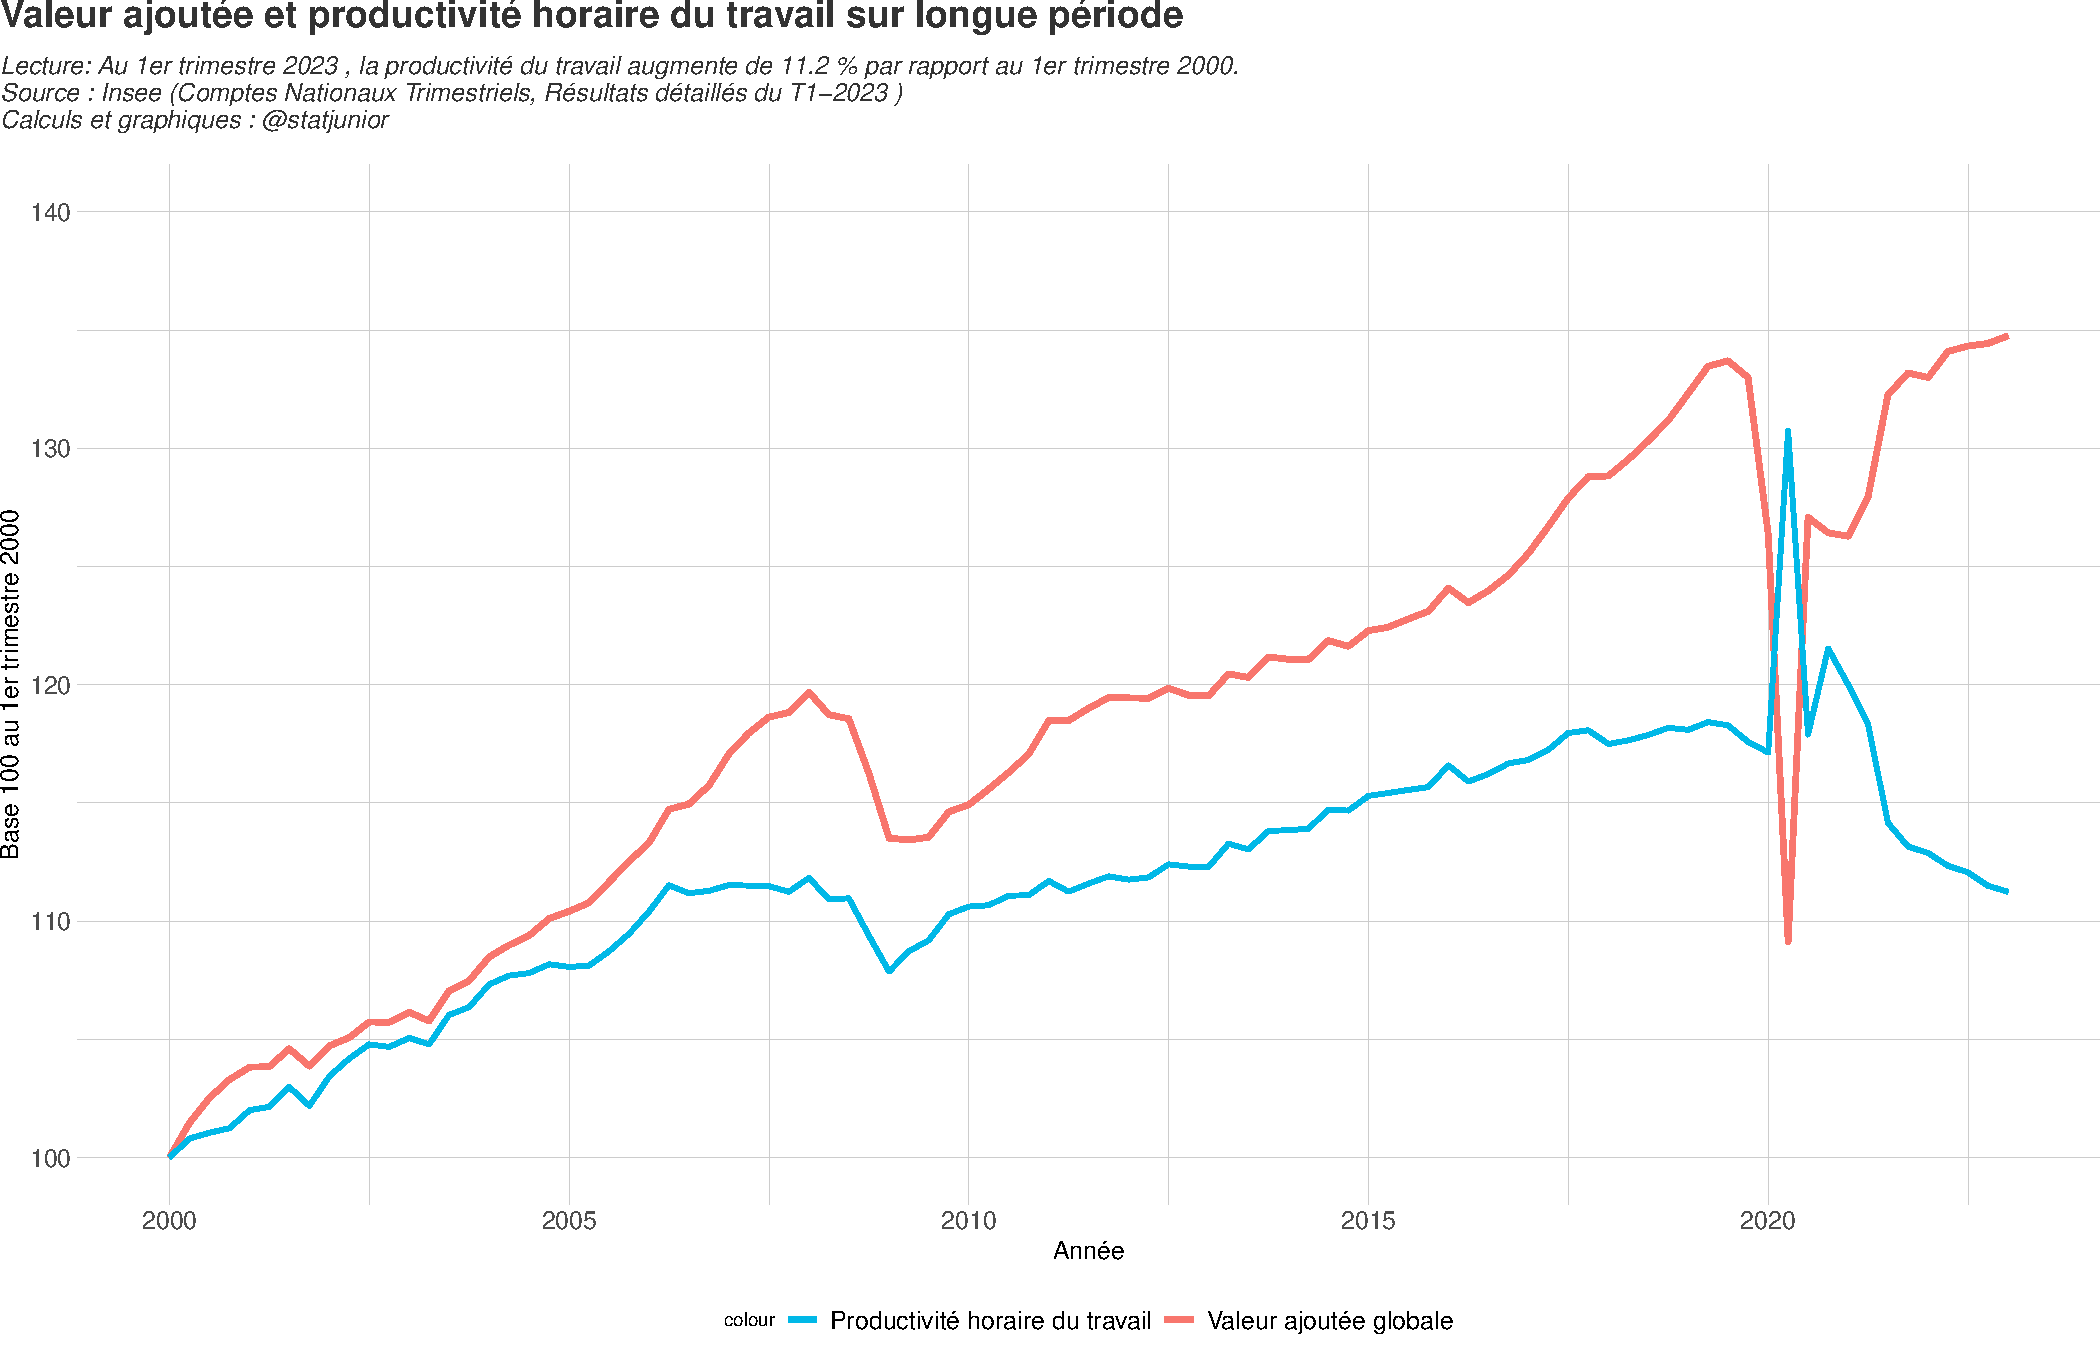
\includegraphics[keepaspectratio]{rapport_pdf_compte_branche_files/figure-latex/unnamed-chunk-10-1.pdf}}

\subsection{Evolution des prix de production par branche depuis
2019}\label{evolution-des-prix-de-production-par-branche-depuis-2019}

\subsection{Evolution des prix de valeur ajoutée par branche depuis
2019}\label{evolution-des-prix-de-valeur-ajoutuxe9e-par-branche-depuis-2019}

\subsection{Evolution des prix de consommation par branche depuis
2019}\label{evolution-des-prix-de-consommation-par-branche-depuis-2019}

\newpage

\section{Solde des échanges extérieurs de la
France}\label{solde-des-uxe9changes-extuxe9rieurs-de-la-france}

\begin{verbatim}
##   |                                                                              |                                                                      |   0%  |                                                                              |=================                                                     |  25%  |                                                                              |===================================                                   |  50%  |                                                                              |====================================================                  |  75%  |                                                                              |======================================================================| 100%
\end{verbatim}

\pandocbounded{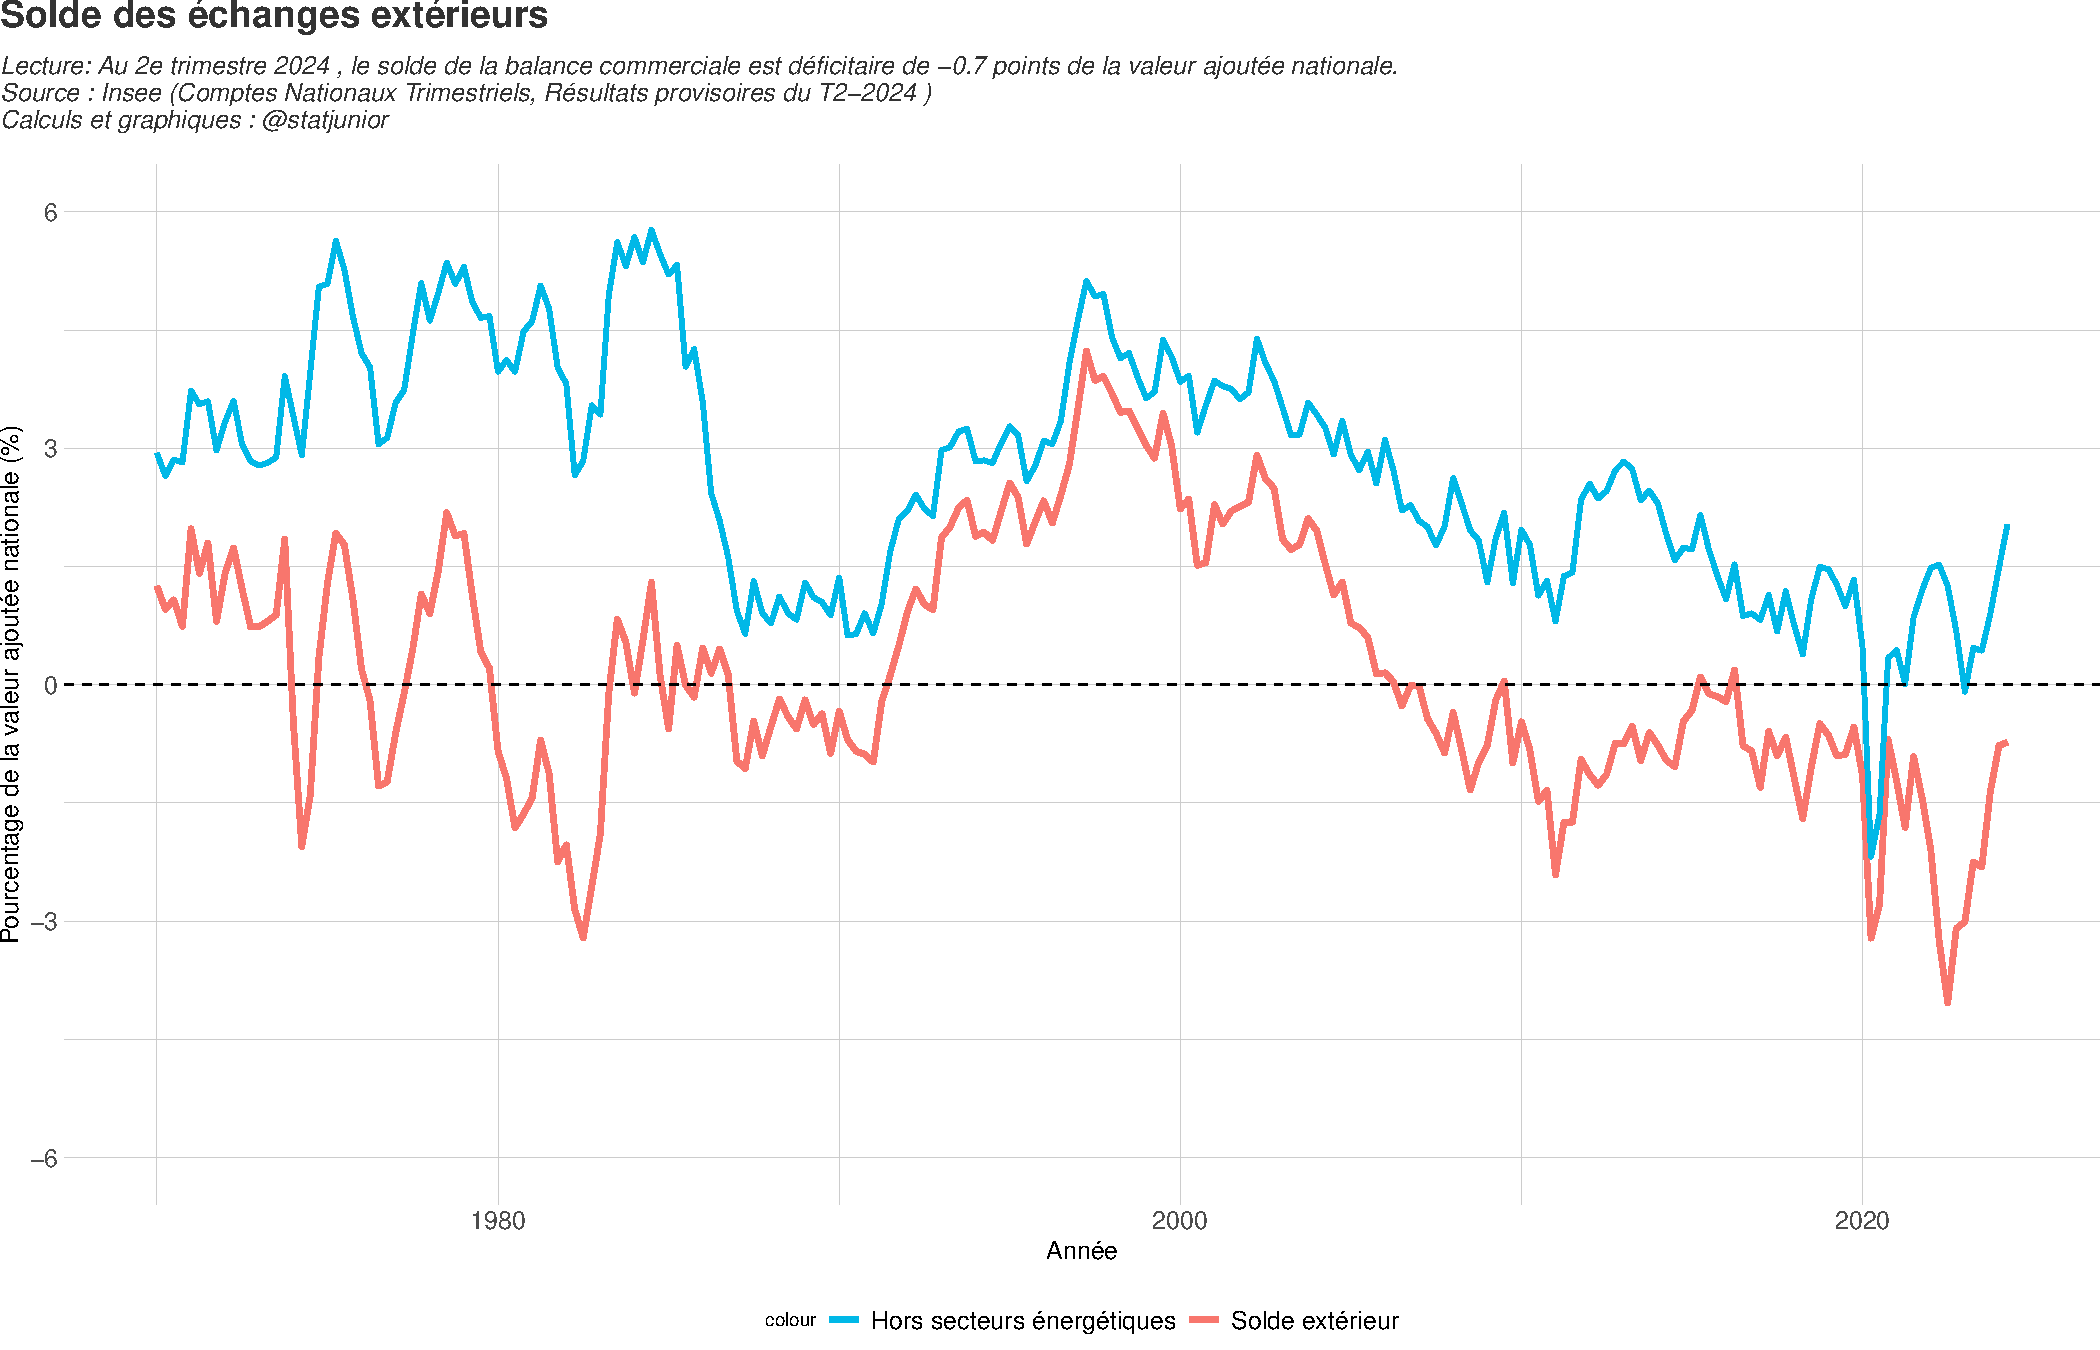
\includegraphics[keepaspectratio]{rapport_pdf_compte_branche_files/figure-latex/unnamed-chunk-11-1.pdf}}

\newpage

\section{Consommation des ménages}\label{consommation-des-muxe9nages}

\subsection{Consommation des ménages par branche depuis
2019}\label{consommation-des-muxe9nages-par-branche-depuis-2019}

\pandocbounded{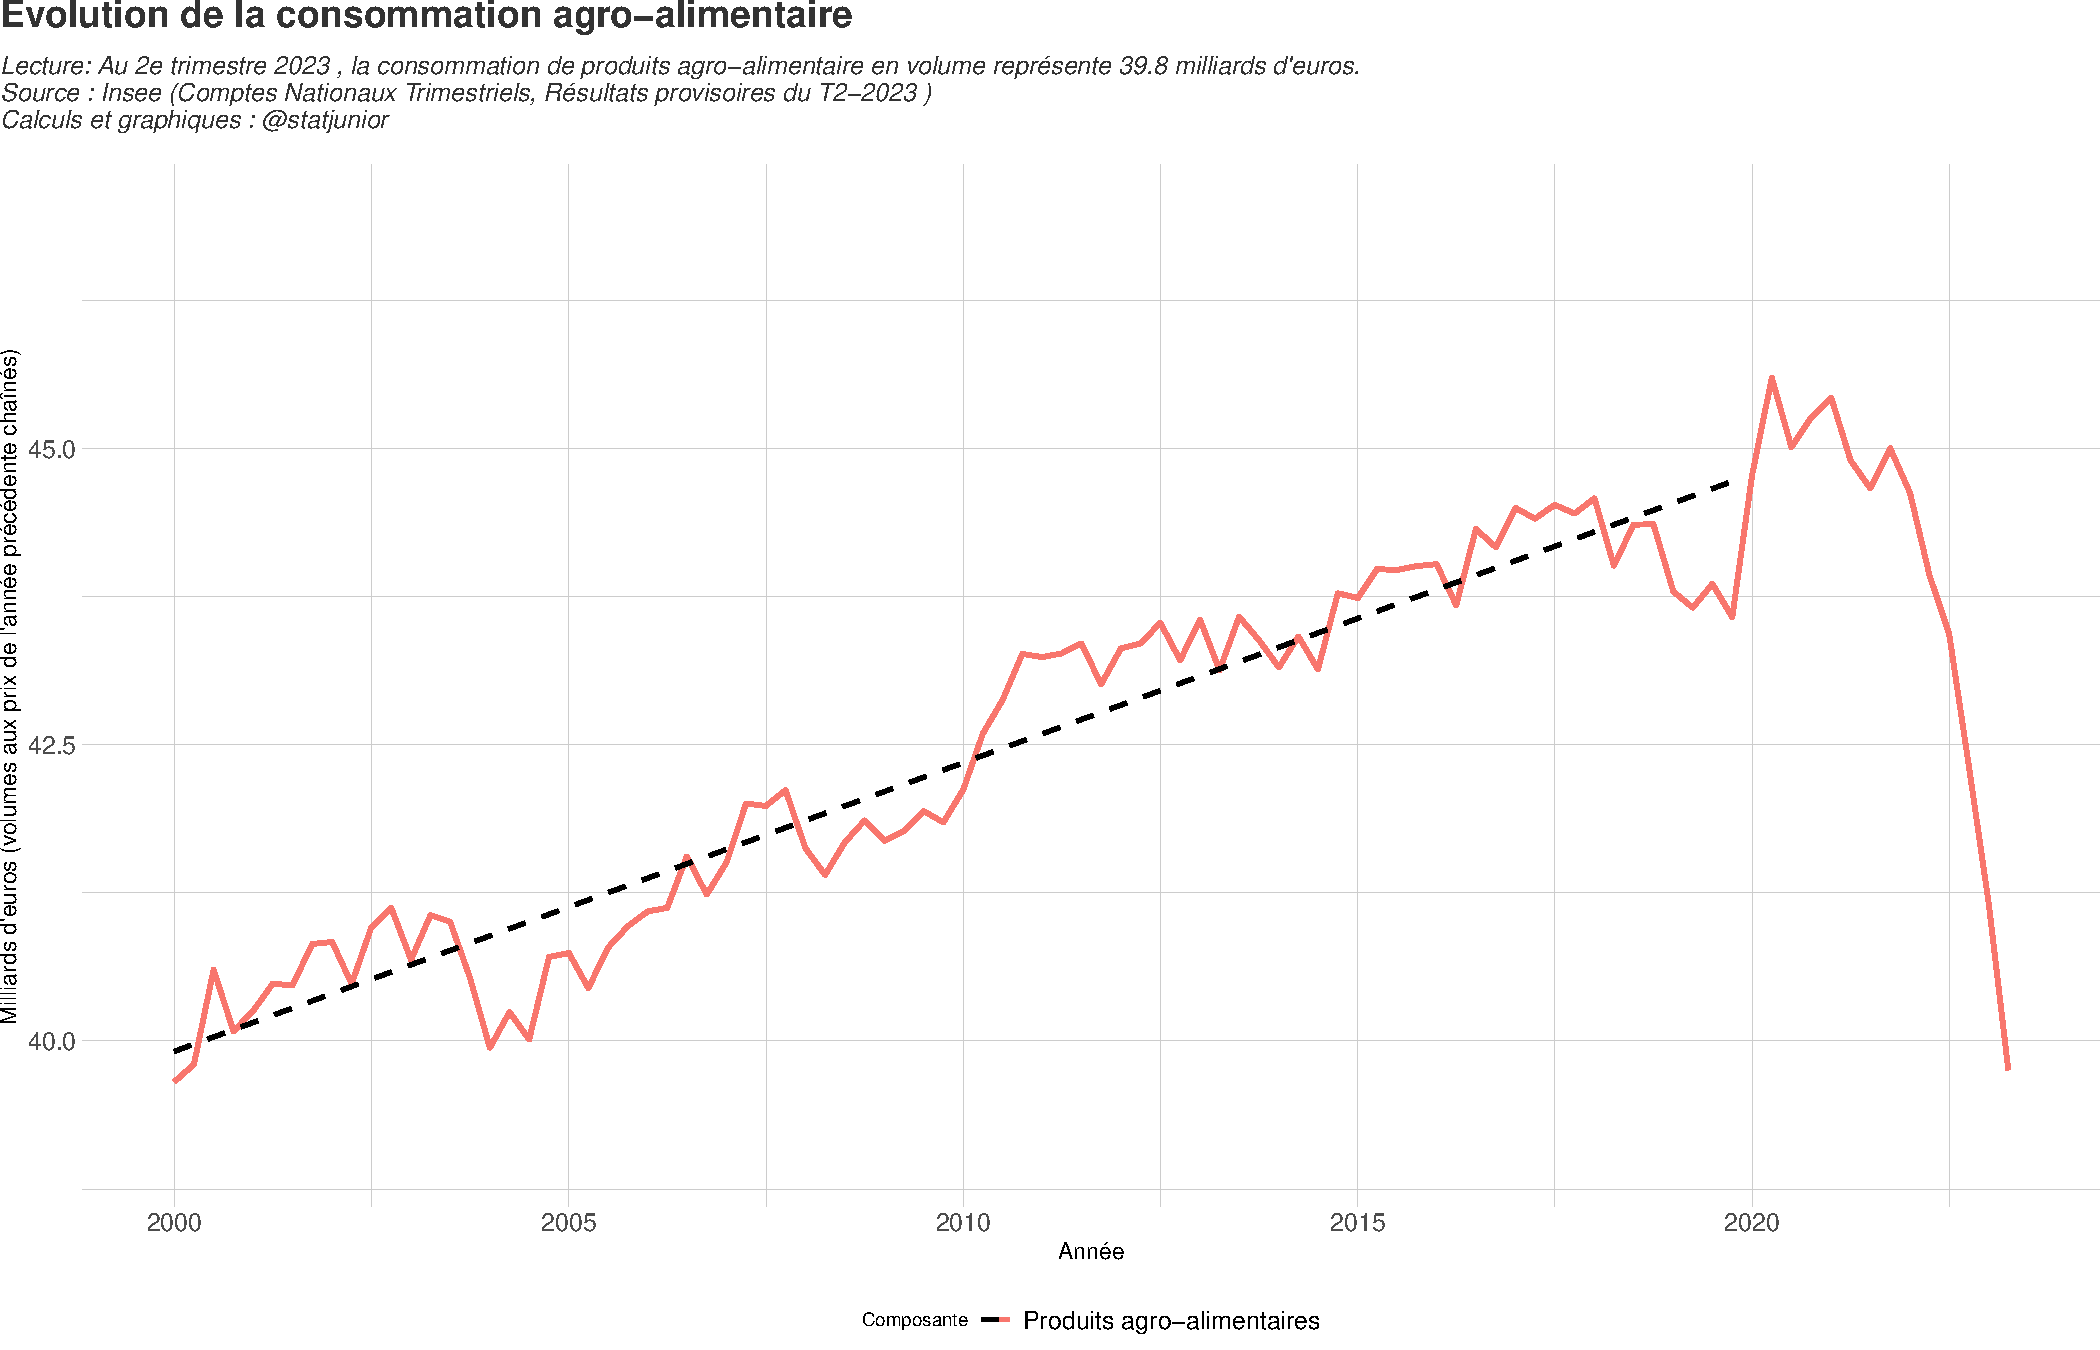
\includegraphics[keepaspectratio]{rapport_pdf_compte_branche_files/figure-latex/unnamed-chunk-13-1.pdf}}

\subsection{Consommation par branche par rapport au dernier trimestre
connu}\label{consommation-par-branche-par-rapport-au-dernier-trimestre-connu}

\pandocbounded{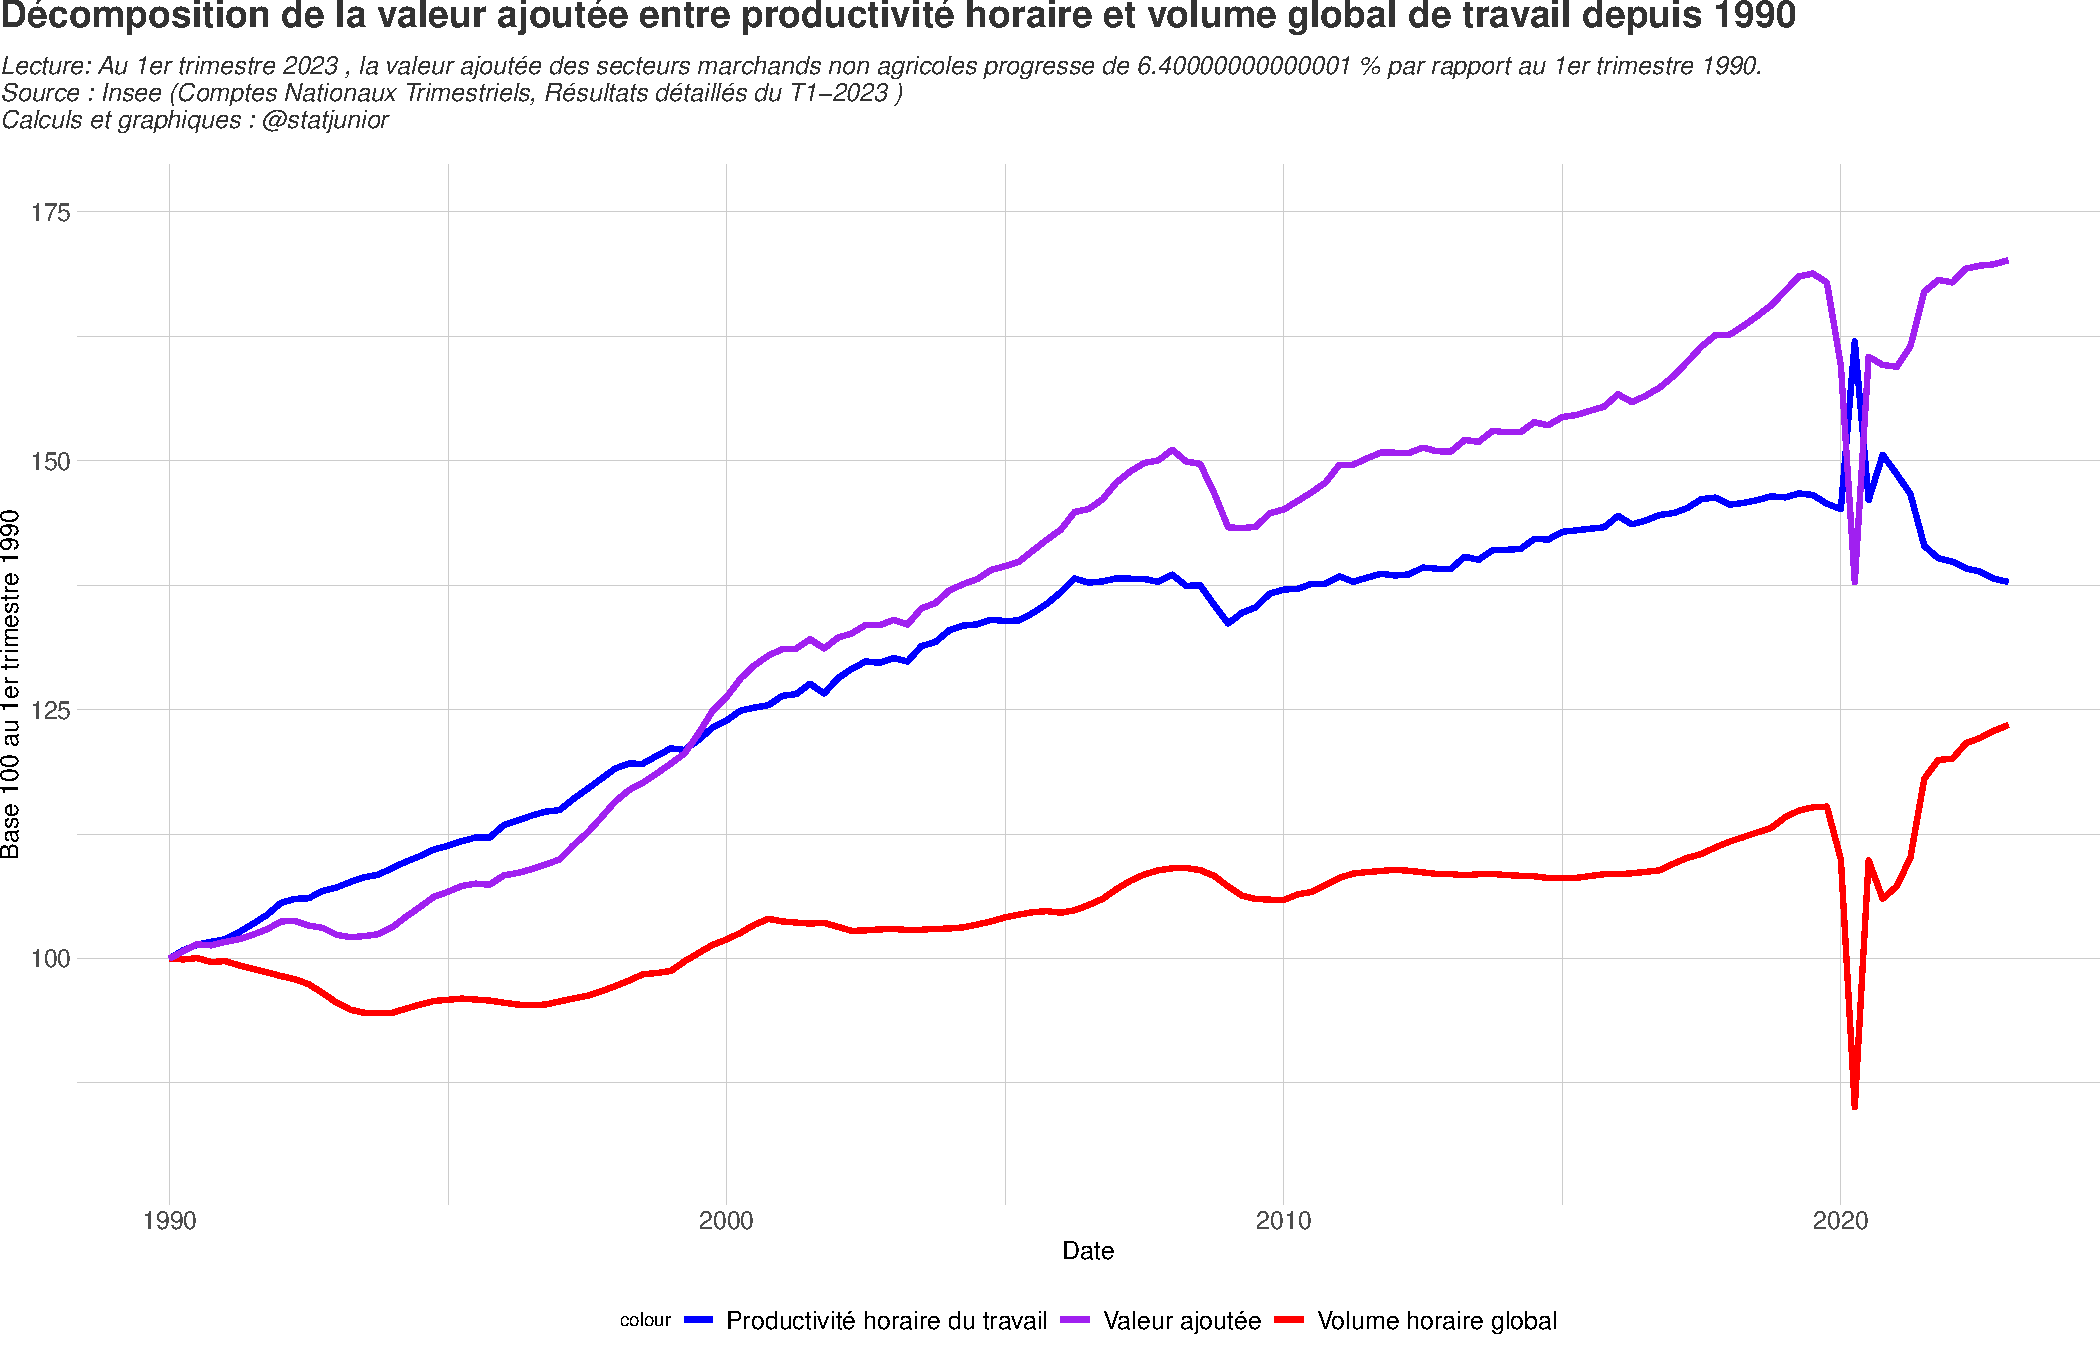
\includegraphics[keepaspectratio]{rapport_pdf_compte_branche_files/figure-latex/unnamed-chunk-14-1.pdf}}

\subsection{Consommation énergétique et agro-alimentaire en volume
depuis fin
2019}\label{consommation-uxe9nerguxe9tique-et-agro-alimentaire-en-volume-depuis-fin-2019}

\pandocbounded{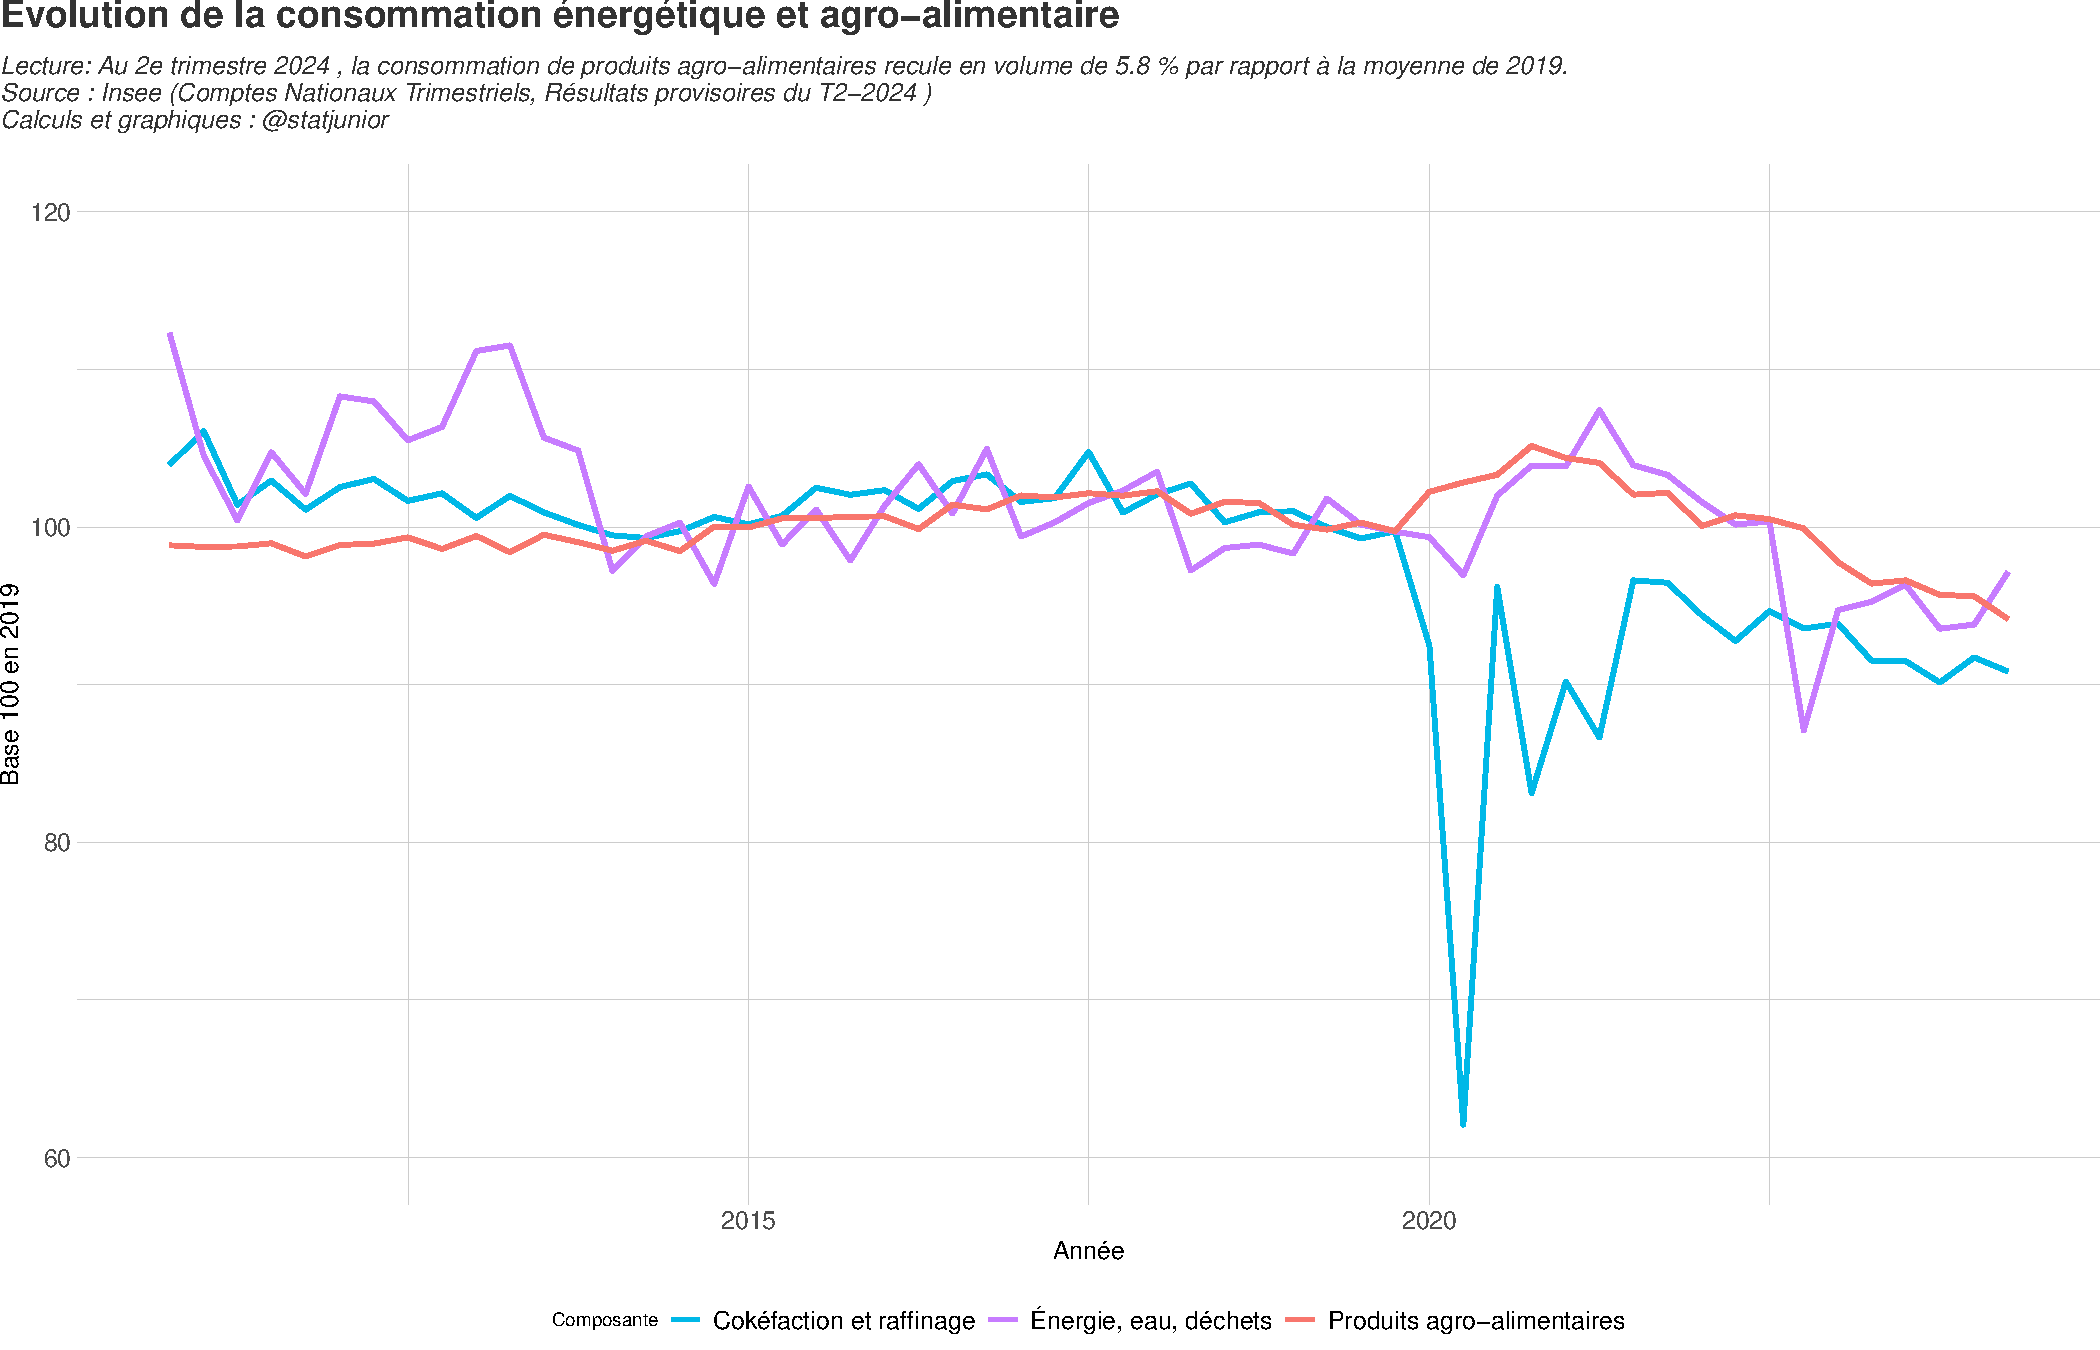
\includegraphics[keepaspectratio]{rapport_pdf_compte_branche_files/figure-latex/unnamed-chunk-15-1.pdf}}

\subsection{Evolution sur longue période de la consommation alimentaire
en
volume}\label{evolution-sur-longue-puxe9riode-de-la-consommation-alimentaire-en-volume}

\pandocbounded{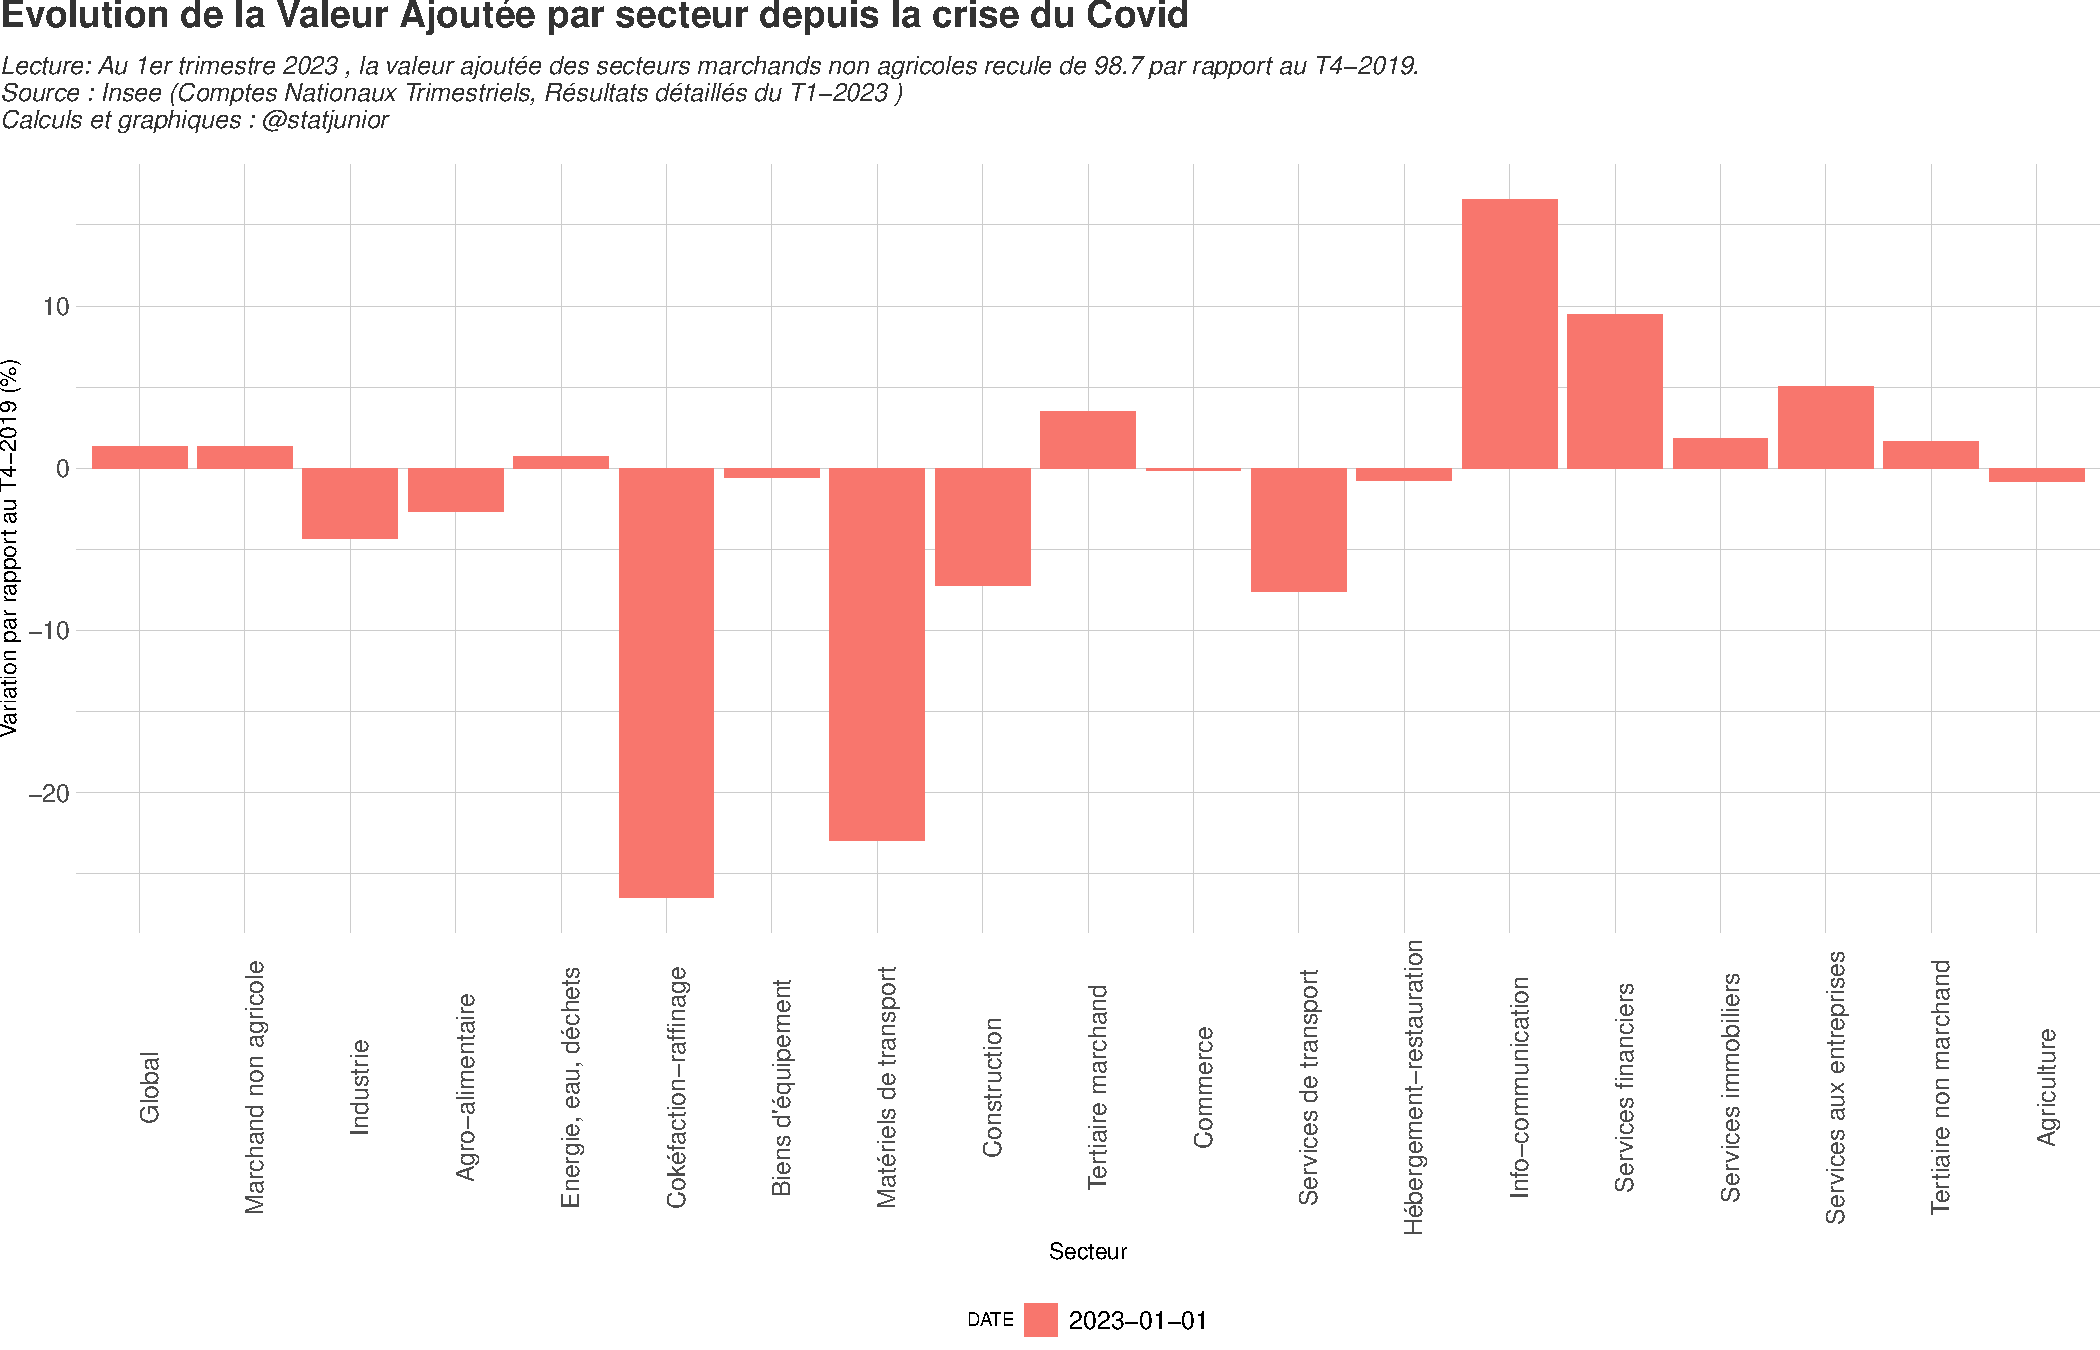
\includegraphics[keepaspectratio]{rapport_pdf_compte_branche_files/figure-latex/unnamed-chunk-16-1.pdf}}

\newpage

\section{Investissement}\label{investissement}

\subsection{Investissement par branche par rapport à
2019}\label{investissement-par-branche-par-rapport-uxe0-2019}

\pandocbounded{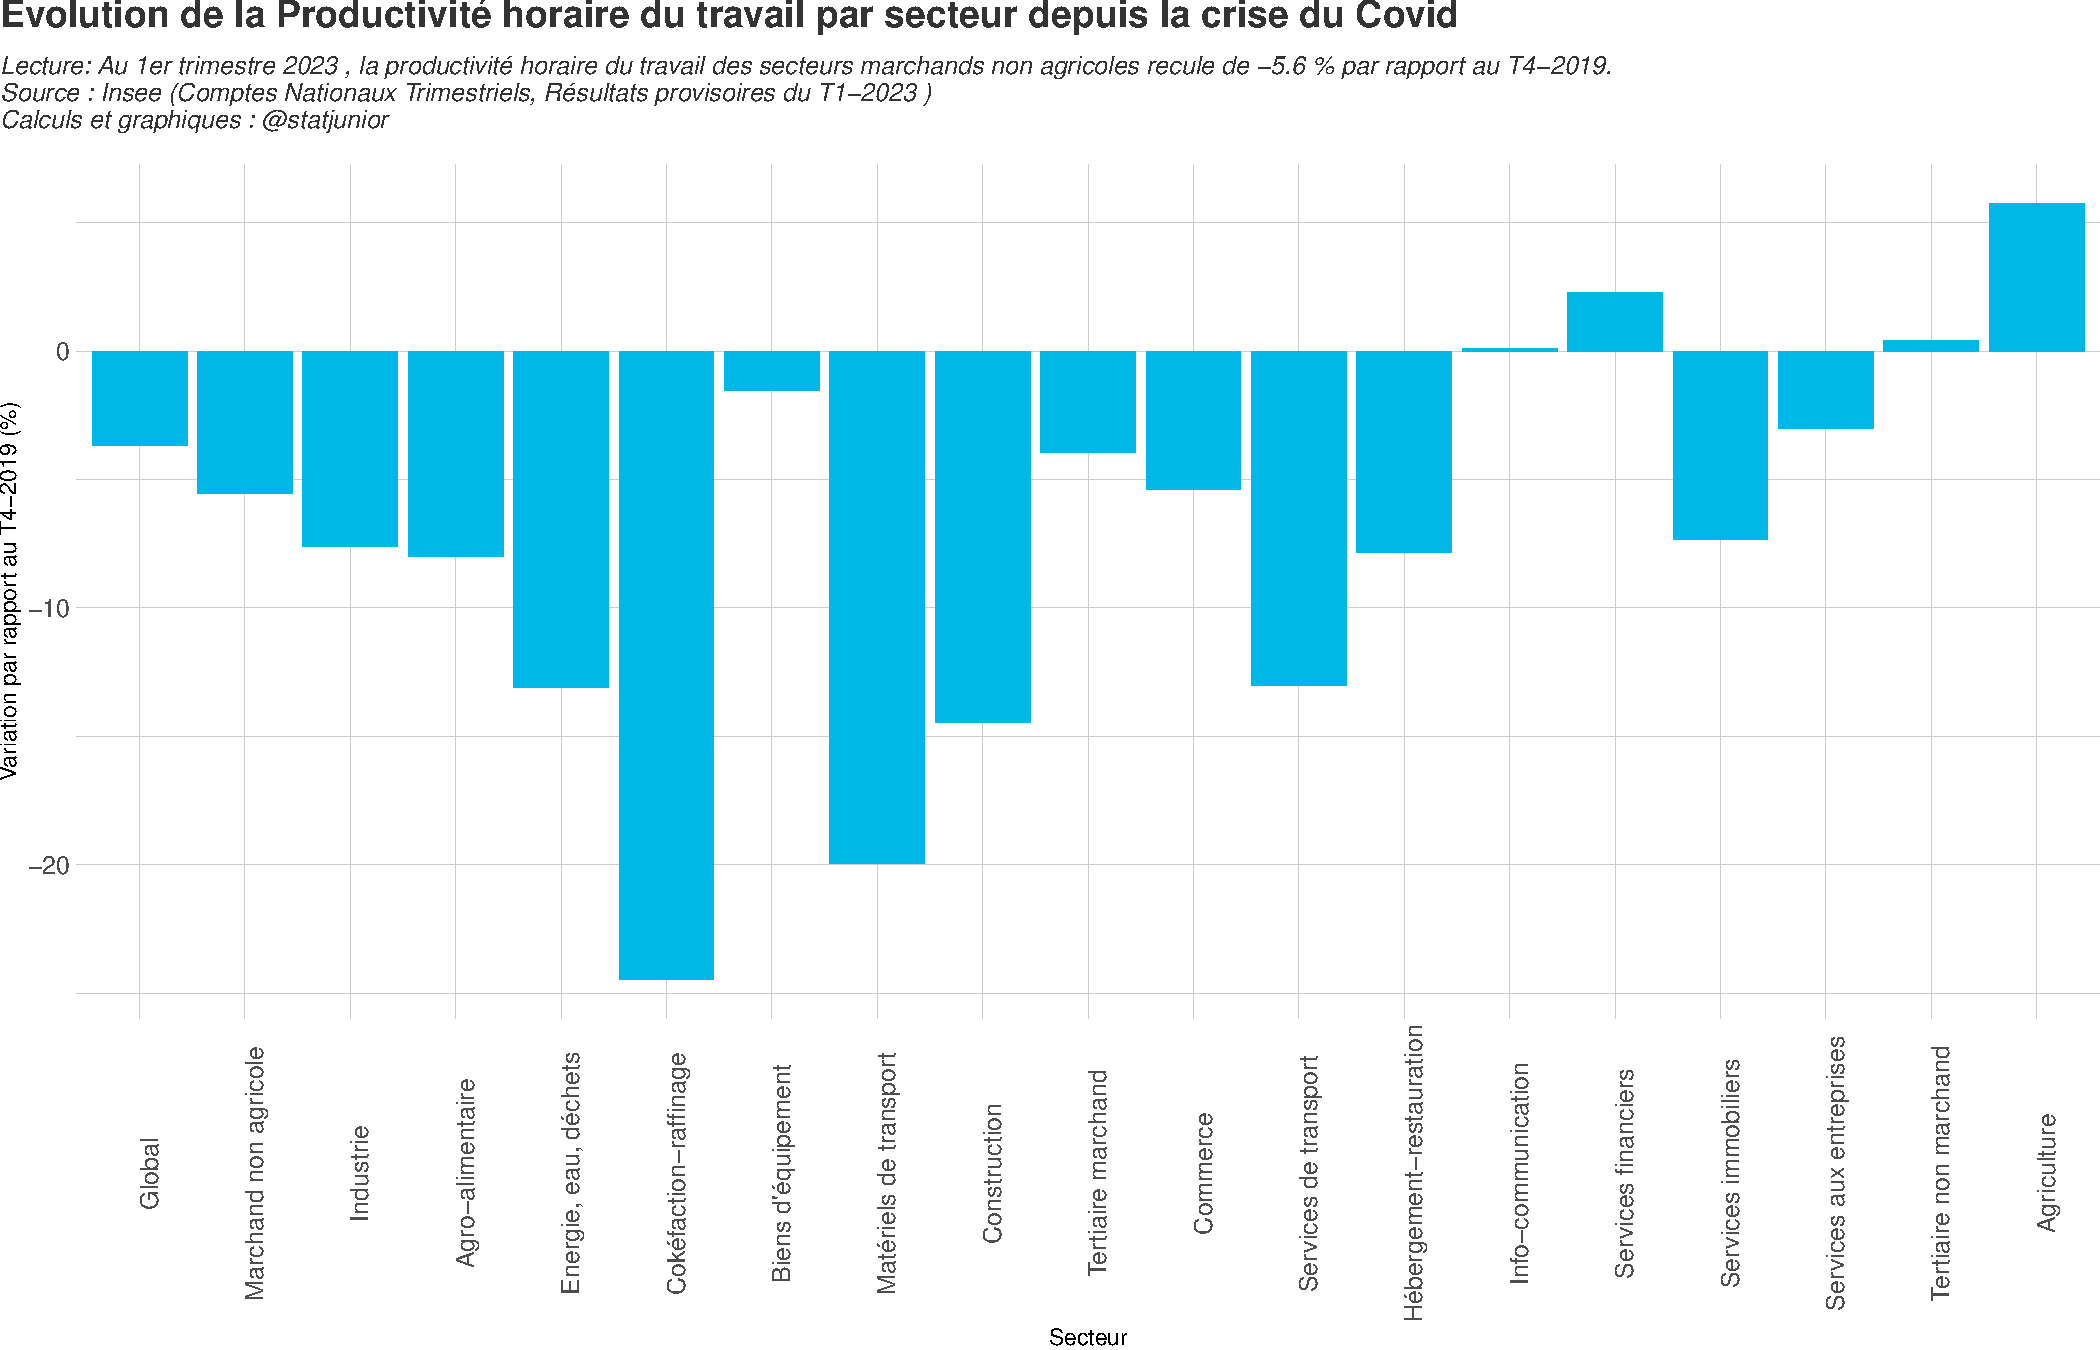
\includegraphics[keepaspectratio]{rapport_pdf_compte_branche_files/figure-latex/unnamed-chunk-18-1.pdf}}

\subsection{Investissement par rapport au dernier trimestre
connu}\label{investissement-par-rapport-au-dernier-trimestre-connu}

\pandocbounded{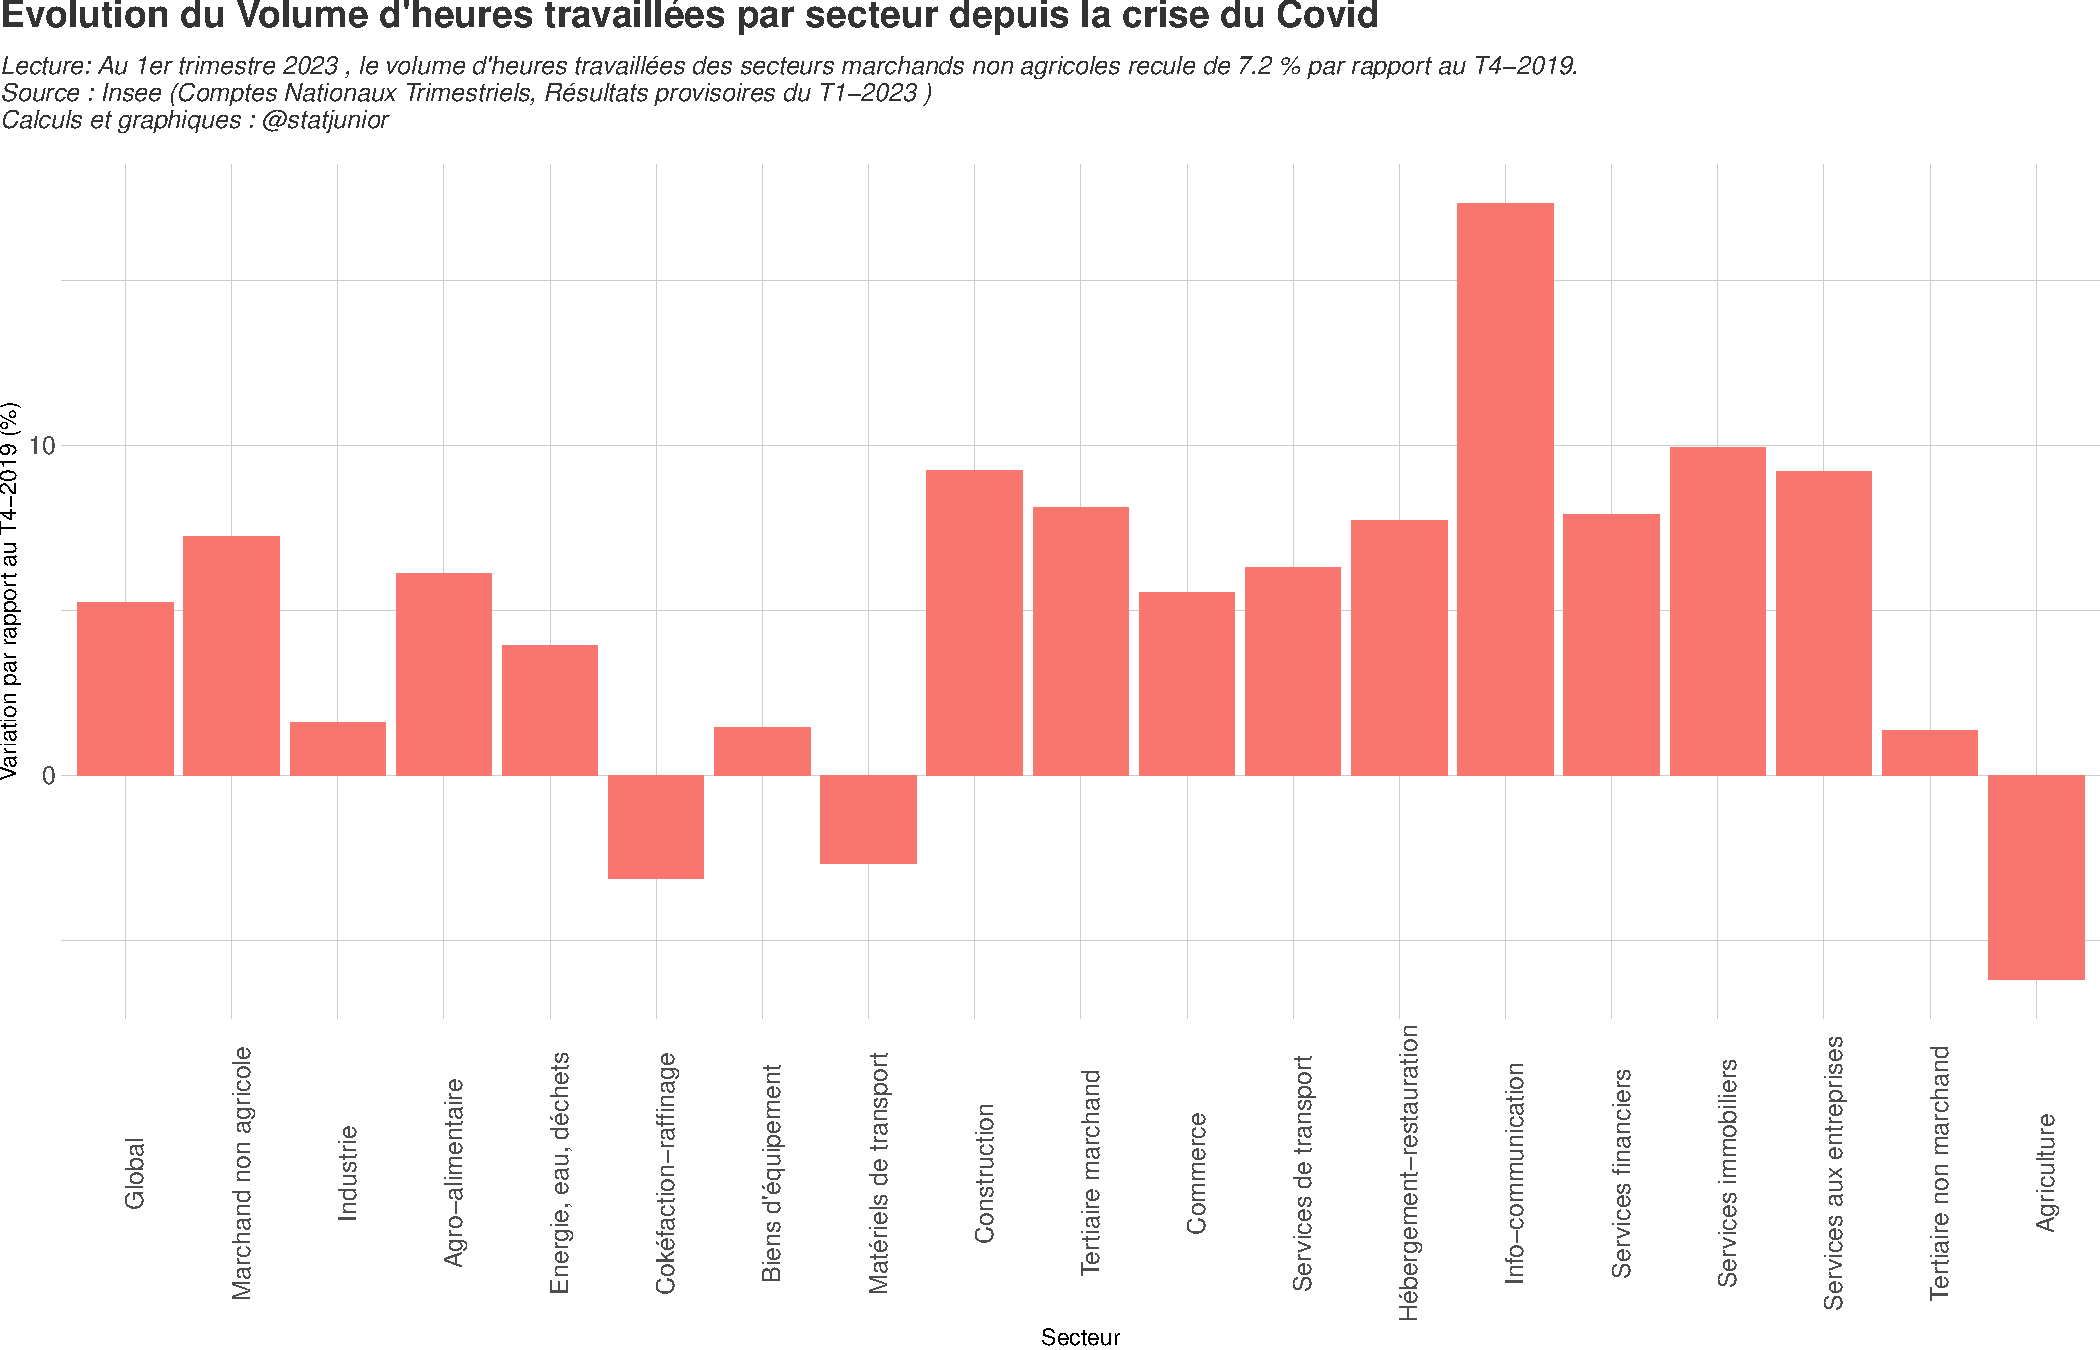
\includegraphics[keepaspectratio]{rapport_pdf_compte_branche_files/figure-latex/unnamed-chunk-19-1.pdf}}

\newpage

\section{Salaires, Masse salariale et Productivité du
travail}\label{salaires-masse-salariale-et-productivituxe9-du-travail}

\subsection{Evolution de la valeur ajoutée et de la productivité du
travail depuis
2000}\label{evolution-de-la-valeur-ajoutuxe9e-et-de-la-productivituxe9-du-travail-depuis-2000}

\pandocbounded{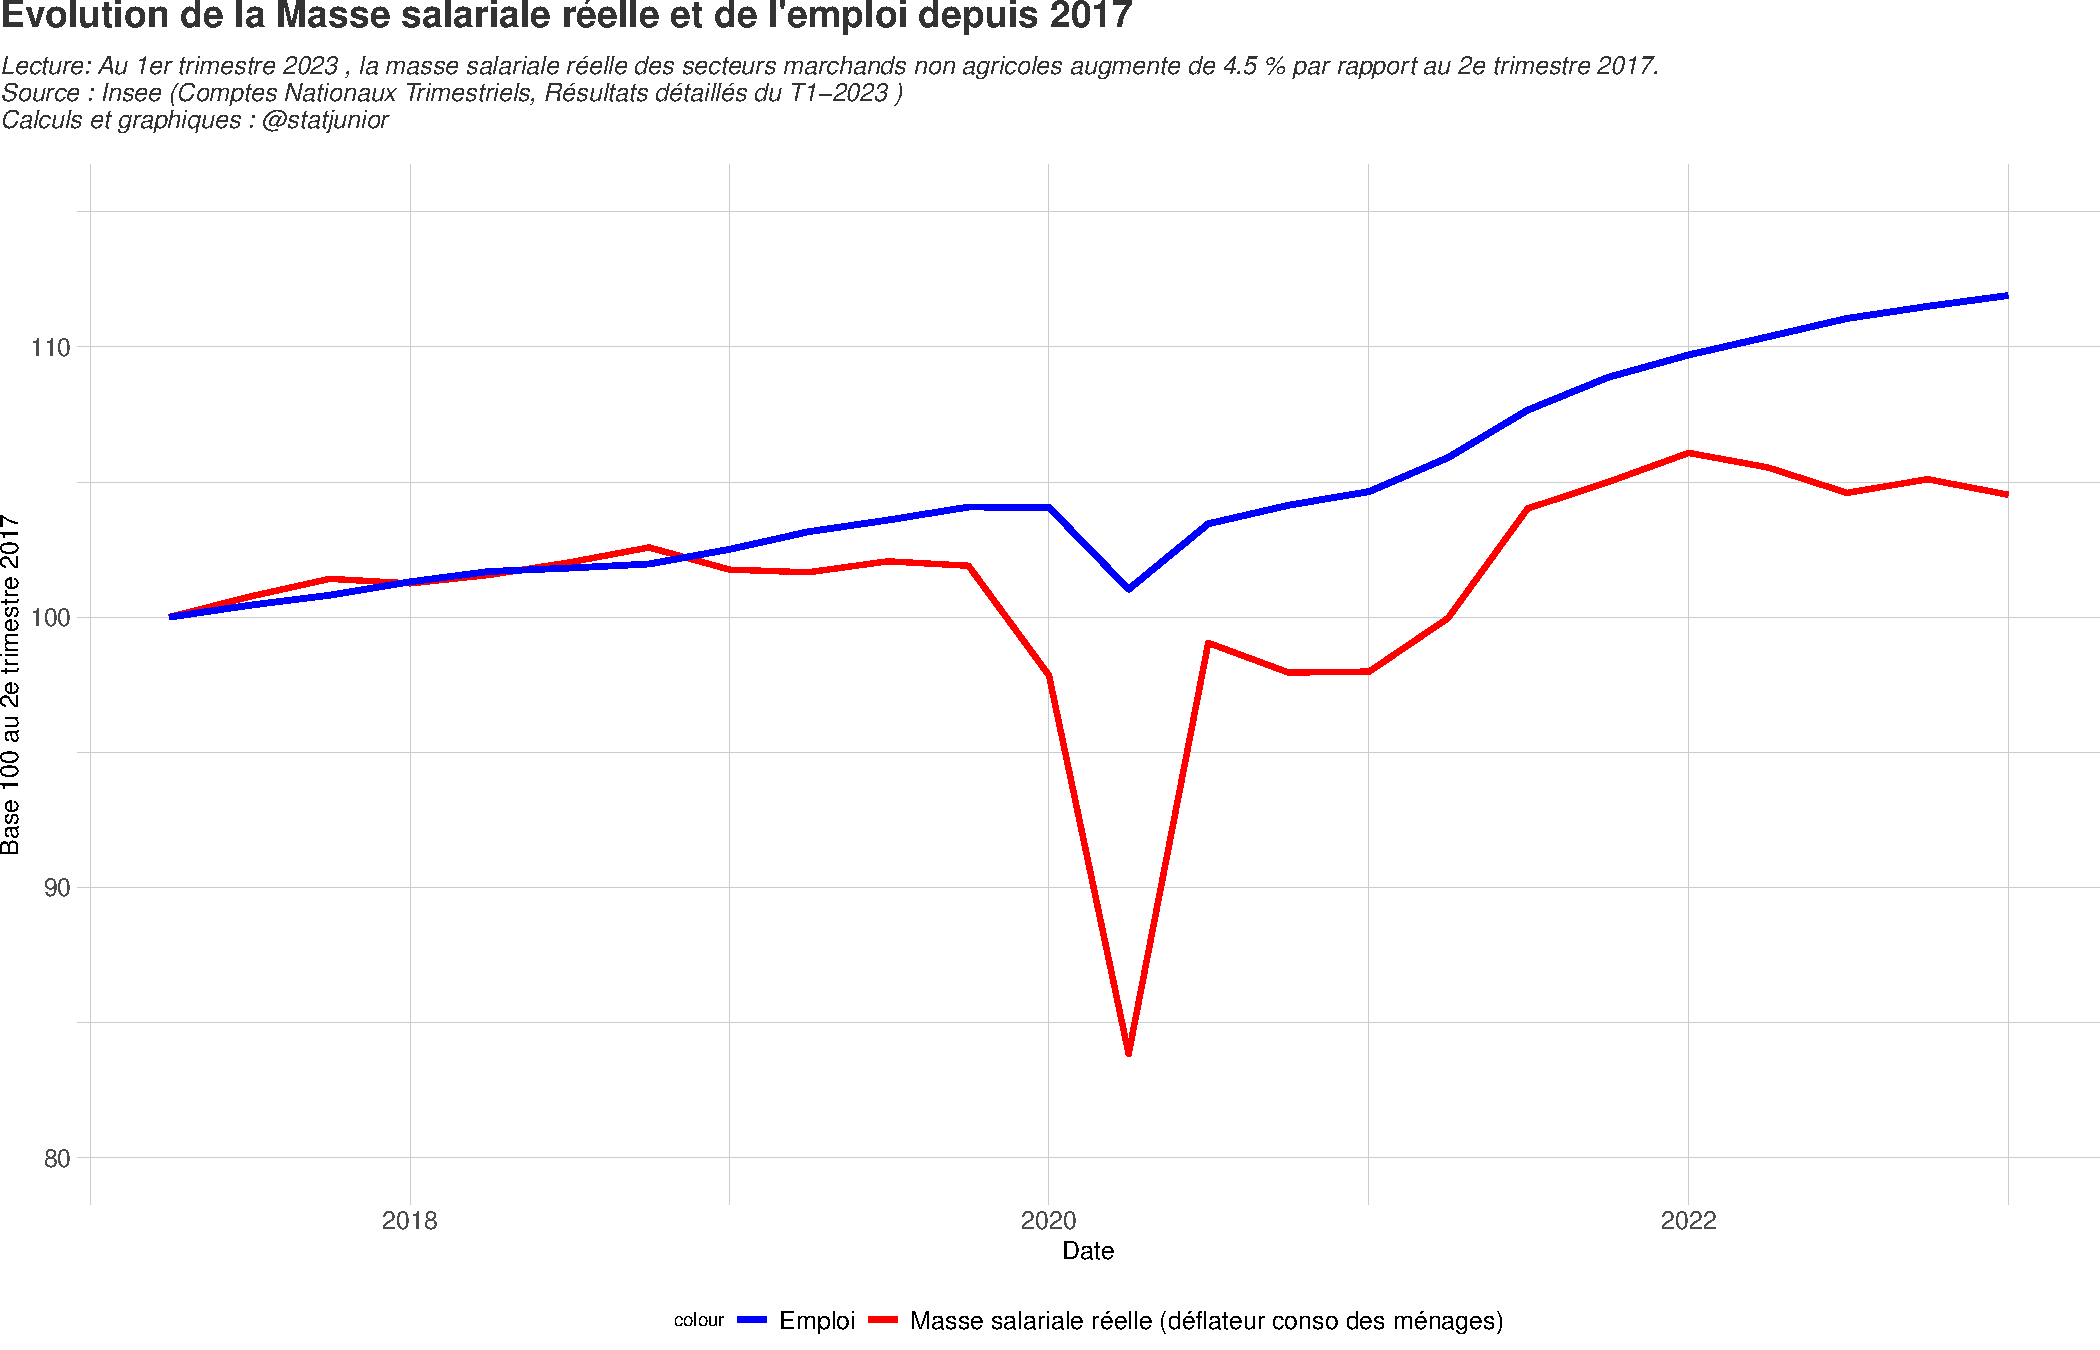
\includegraphics[keepaspectratio]{rapport_pdf_compte_branche_files/figure-latex/unnamed-chunk-20-1.pdf}}

\subsection{Evolution de la valeur ajoutée et de la productivité du
travail depuis
2019}\label{evolution-de-la-valeur-ajoutuxe9e-et-de-la-productivituxe9-du-travail-depuis-2019}

\pandocbounded{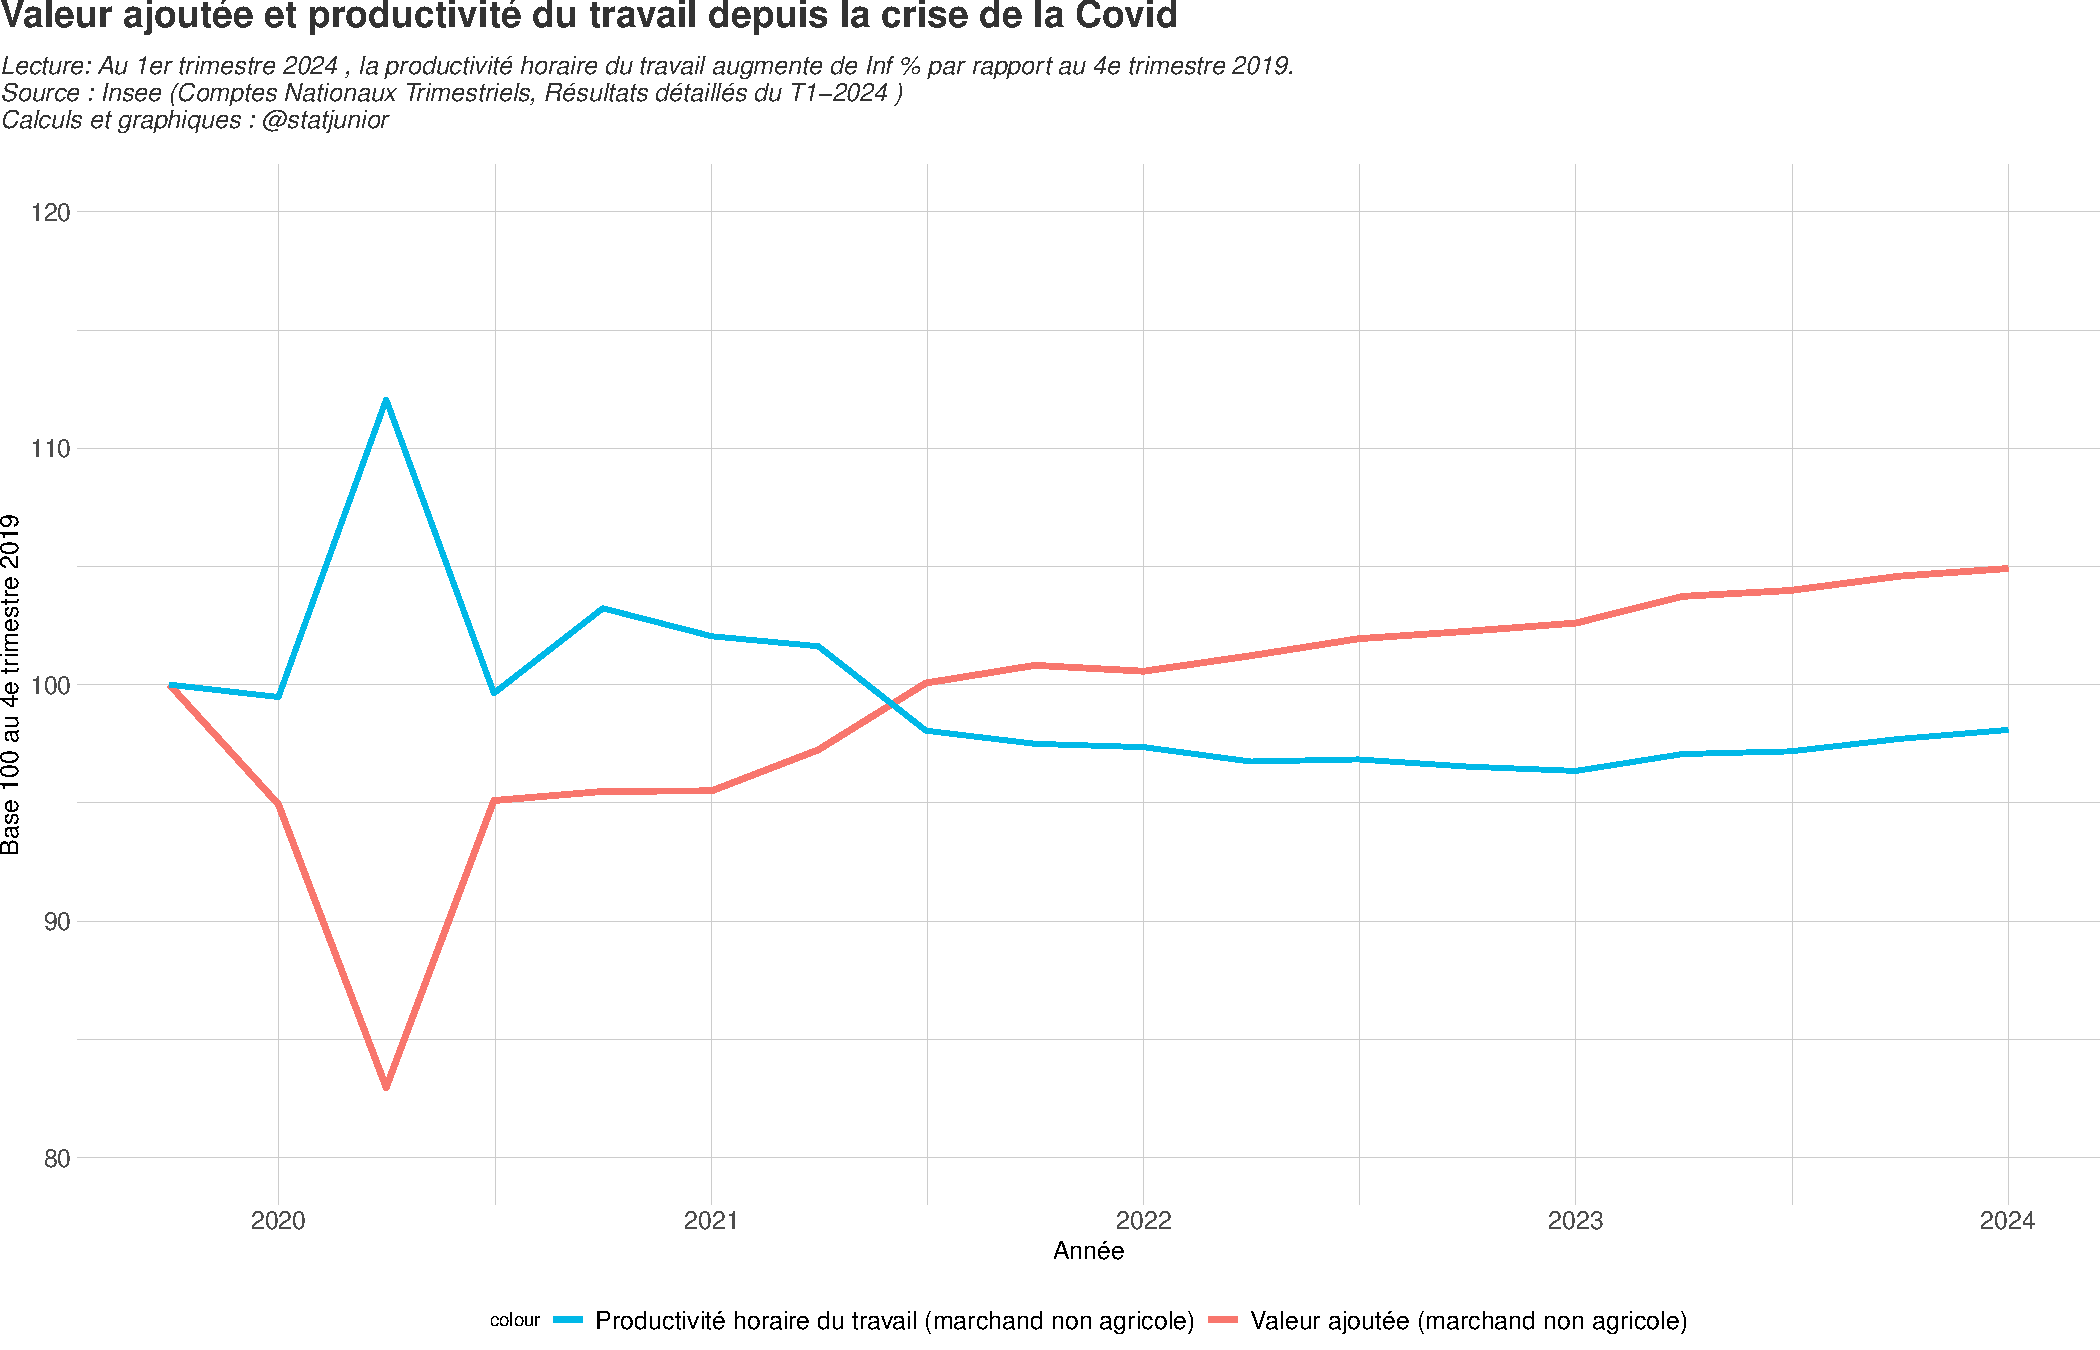
\includegraphics[keepaspectratio]{rapport_pdf_compte_branche_files/figure-latex/unnamed-chunk-21-1.pdf}}

\subsection{Evolution de la Productivité par Tête et de la Productivité
apparente du travail depuis
2019}\label{evolution-de-la-productivituxe9-par-tuxeate-et-de-la-productivituxe9-apparente-du-travail-depuis-2019}

\pandocbounded{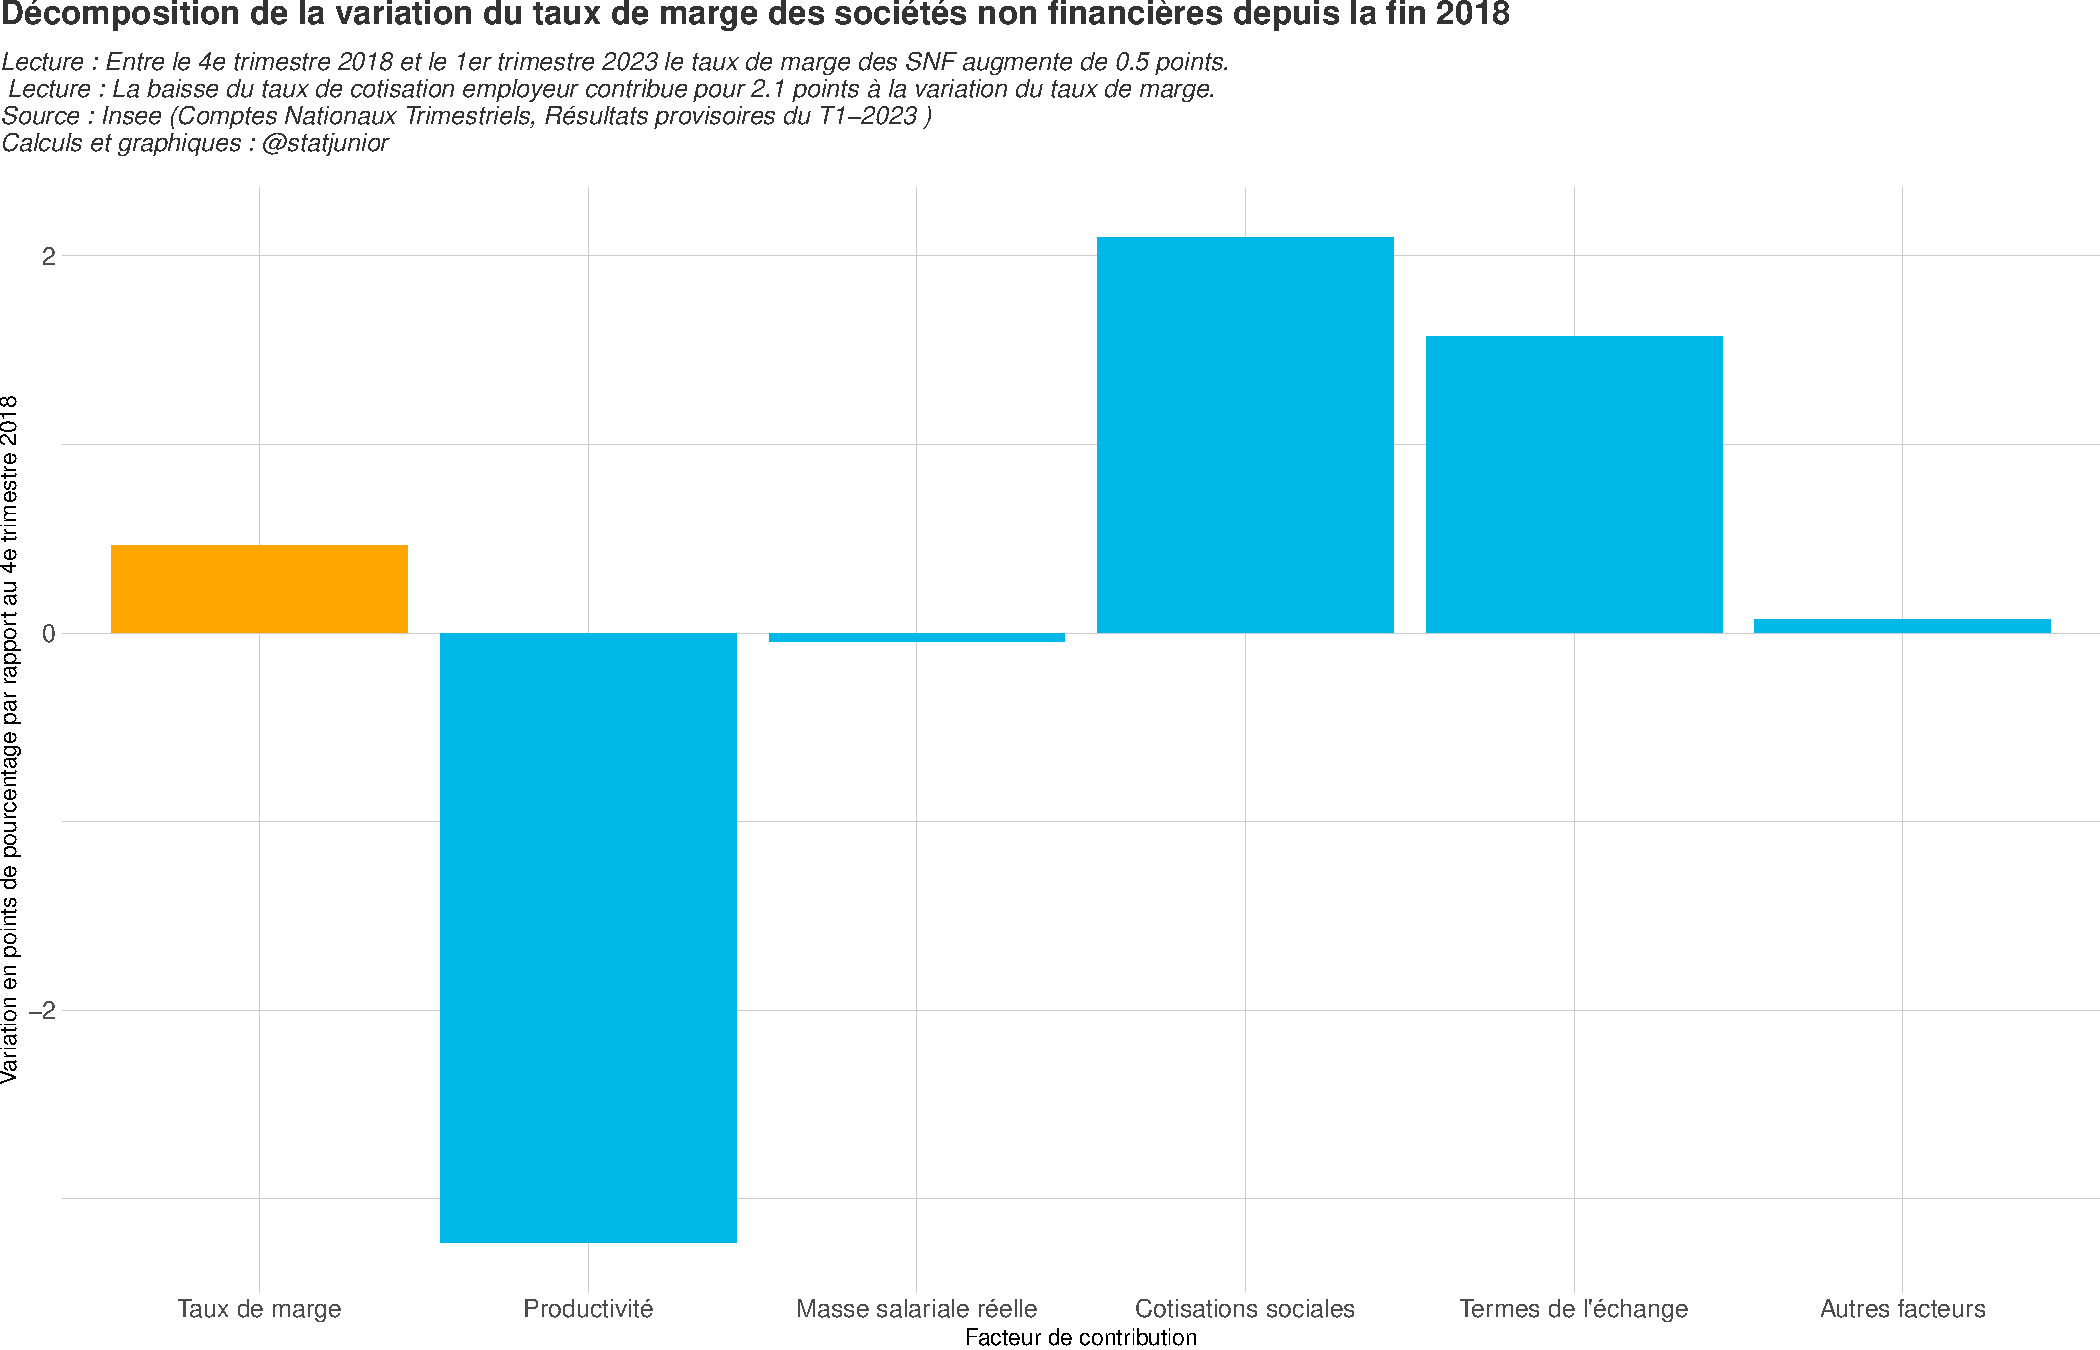
\includegraphics[keepaspectratio]{rapport_pdf_compte_branche_files/figure-latex/unnamed-chunk-22-1.pdf}}

\subsection{Evolution de la masse salariale réelle et de l'emploi depuis
2017}\label{evolution-de-la-masse-salariale-ruxe9elle-et-de-lemploi-depuis-2017}

\pandocbounded{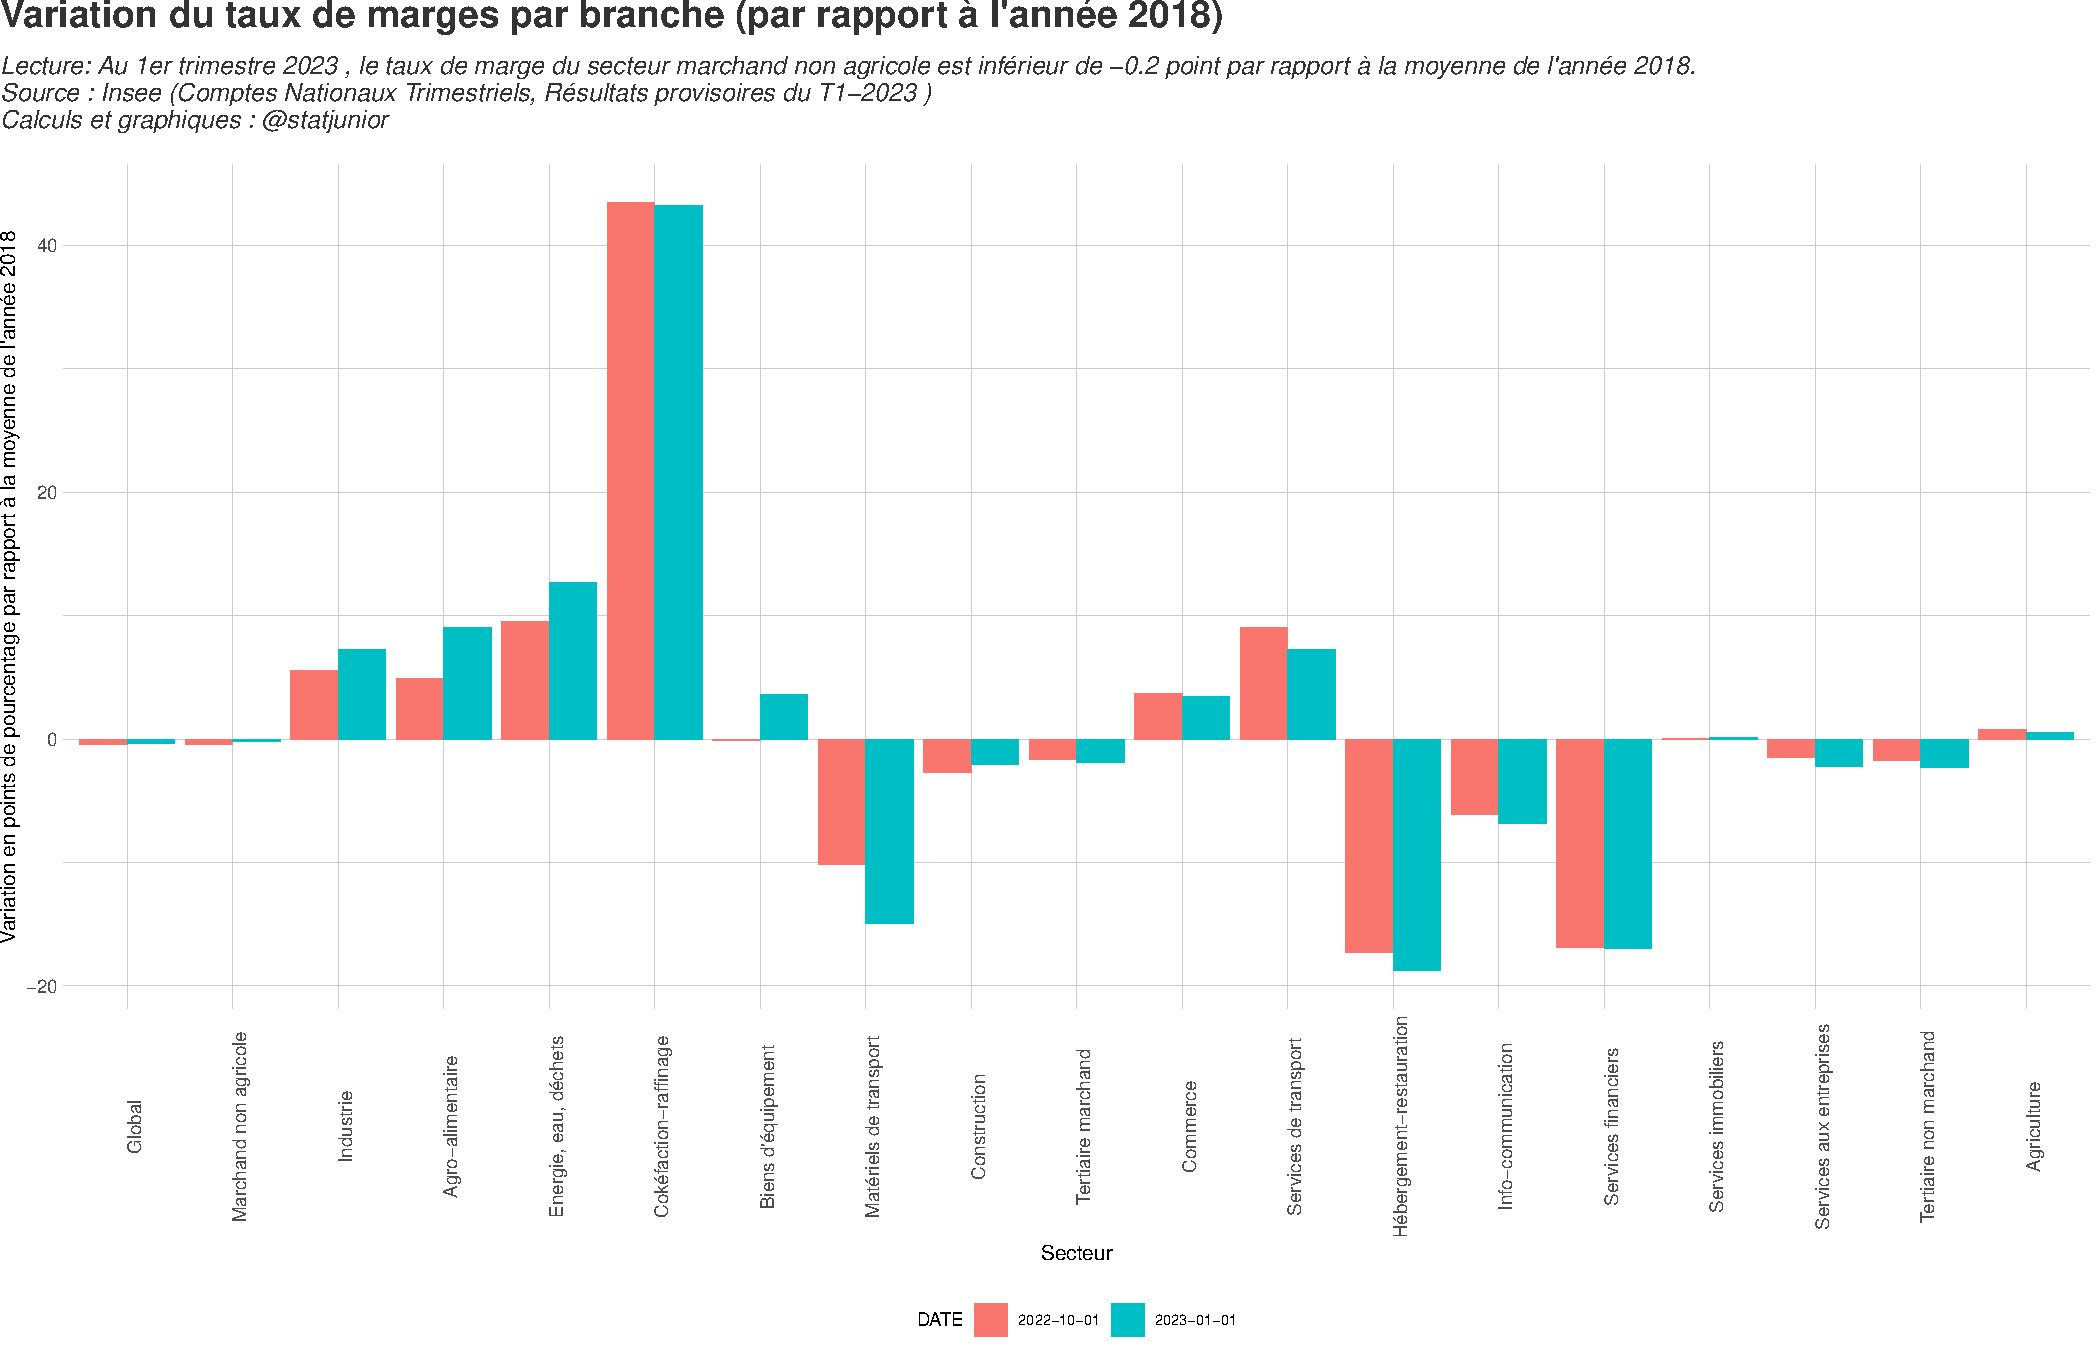
\includegraphics[keepaspectratio]{rapport_pdf_compte_branche_files/figure-latex/unnamed-chunk-23-1.pdf}}

\subsection{Volume de travail global et productivité du travail depuis
1990}\label{volume-de-travail-global-et-productivituxe9-du-travail-depuis-1990}

\pandocbounded{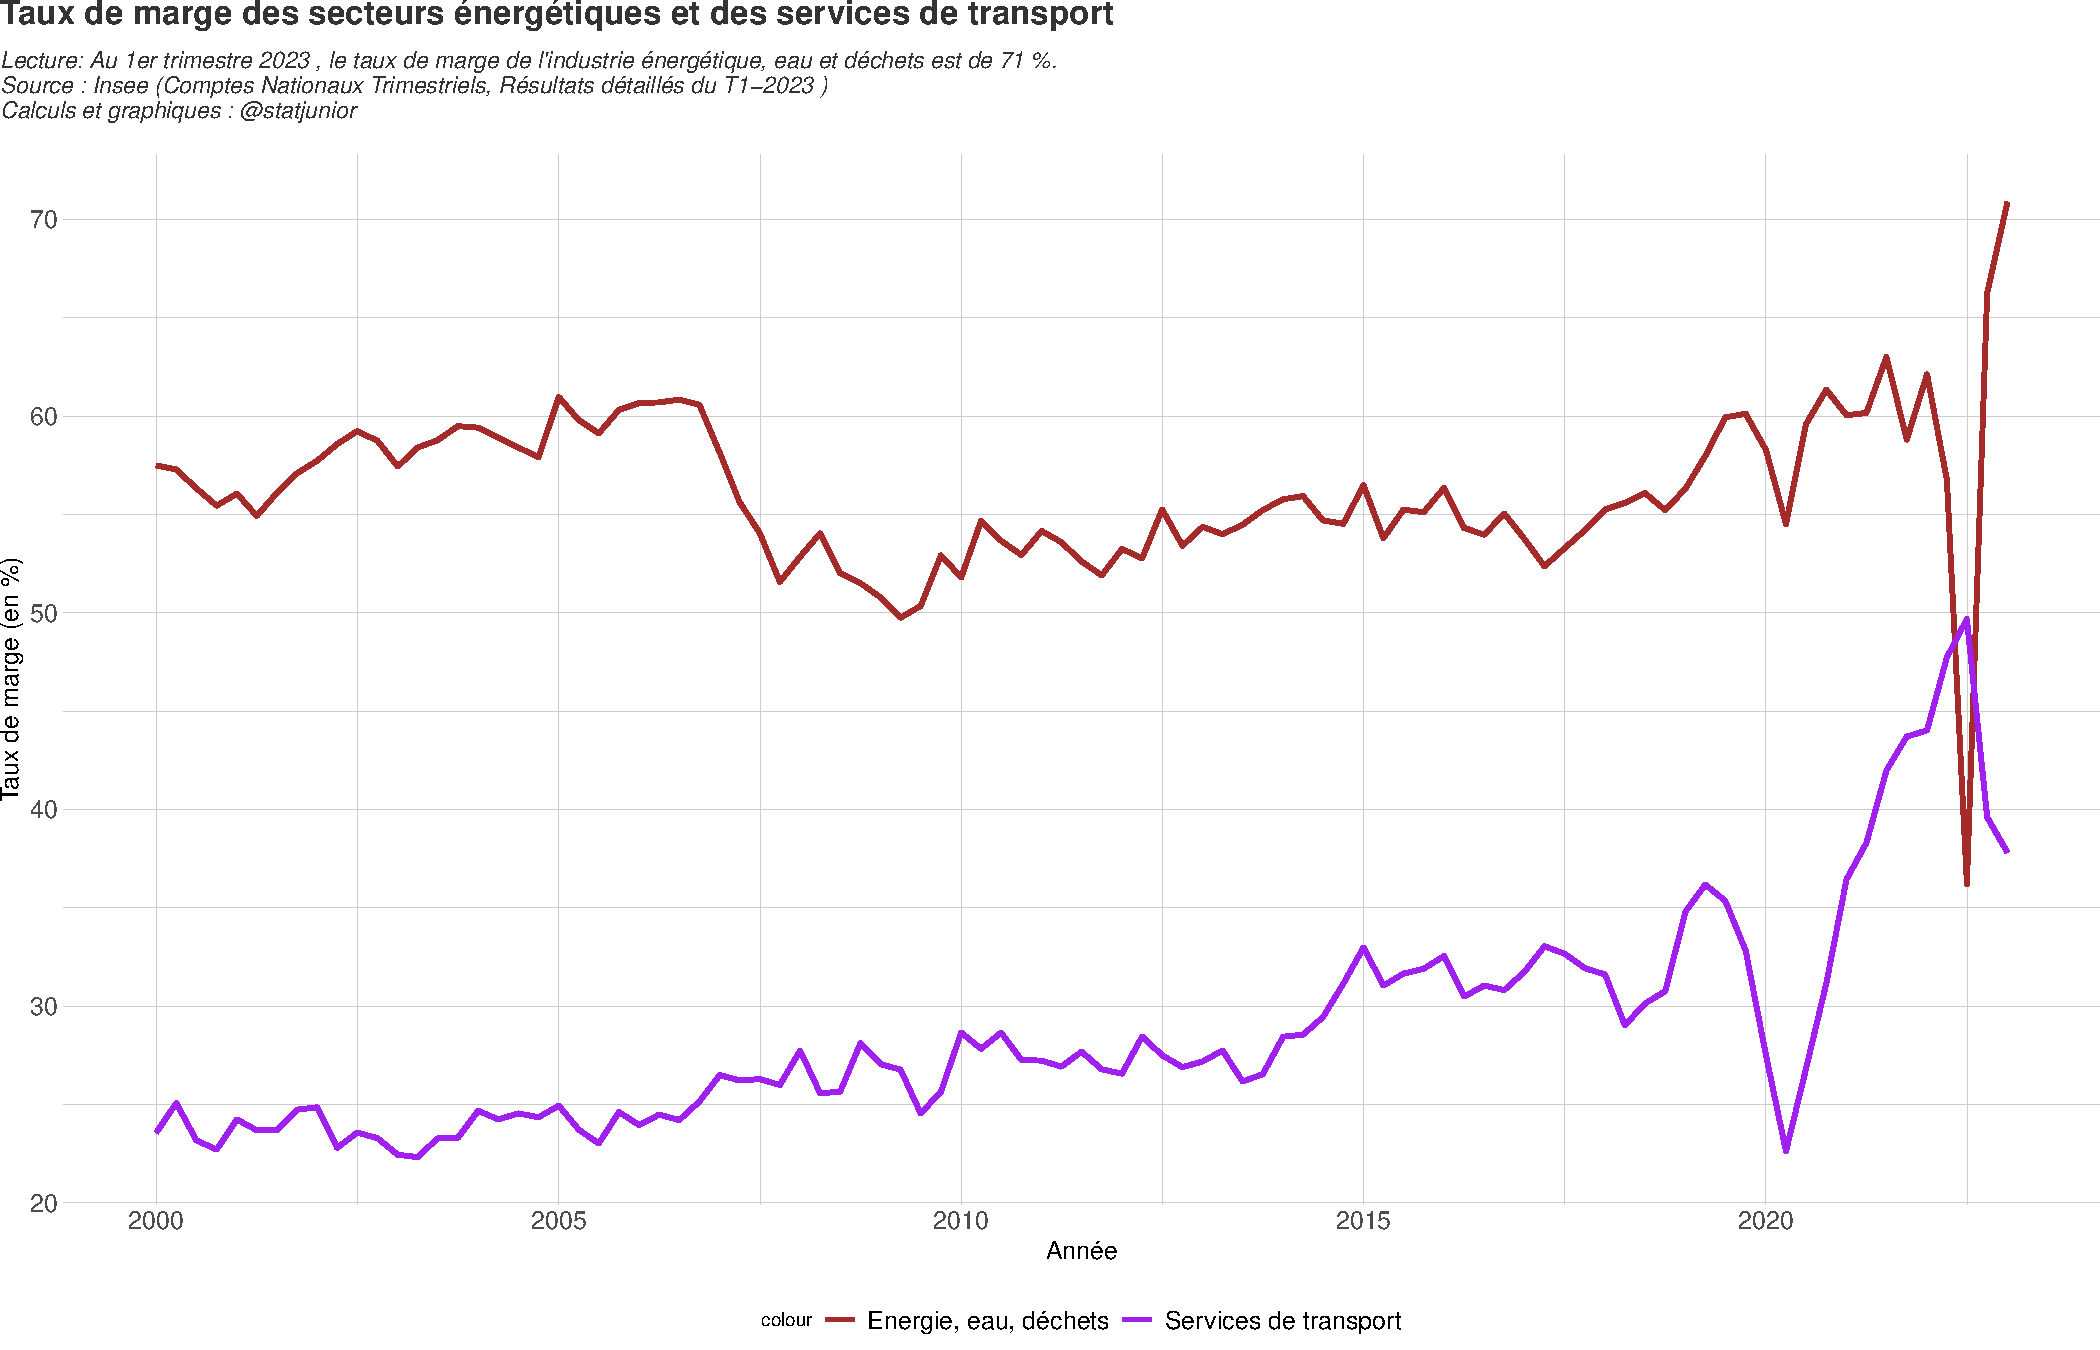
\includegraphics[keepaspectratio]{rapport_pdf_compte_branche_files/figure-latex/unnamed-chunk-24-1.pdf}}

\subsection{Evolution du Salaire Moyen par Tête et de la Productivité
par tête depuis
1990}\label{evolution-du-salaire-moyen-par-tuxeate-et-de-la-productivituxe9-par-tuxeate-depuis-1990}

\pandocbounded{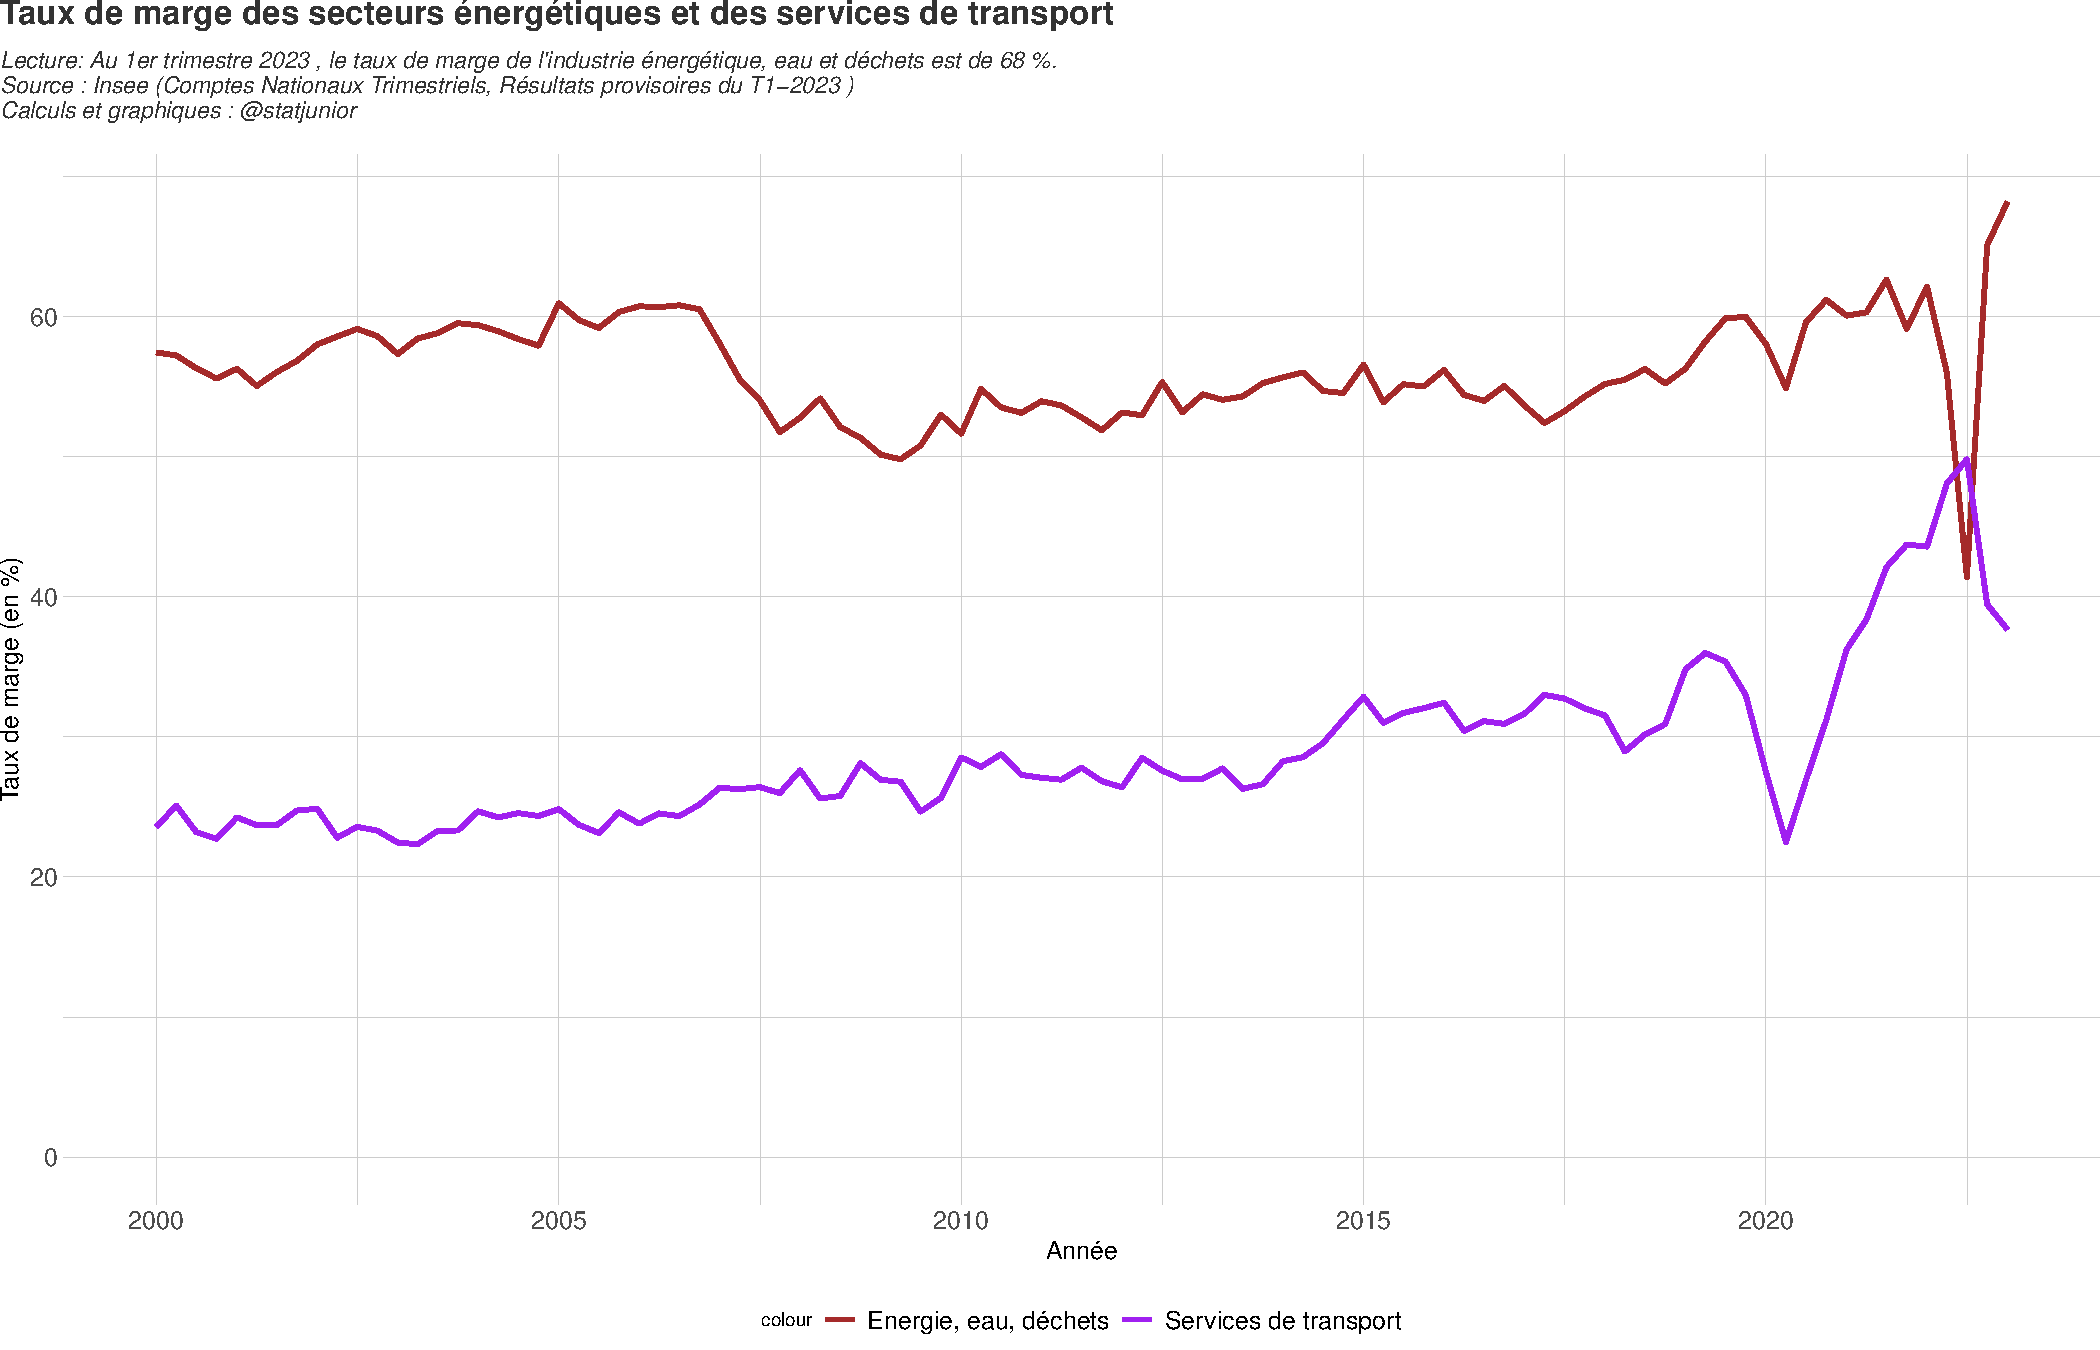
\includegraphics[keepaspectratio]{rapport_pdf_compte_branche_files/figure-latex/unnamed-chunk-25-1.pdf}}

\newpage

\subsection{Productivité du travail sectorielle depuis
2019}\label{productivituxe9-du-travail-sectorielle-depuis-2019}

\pandocbounded{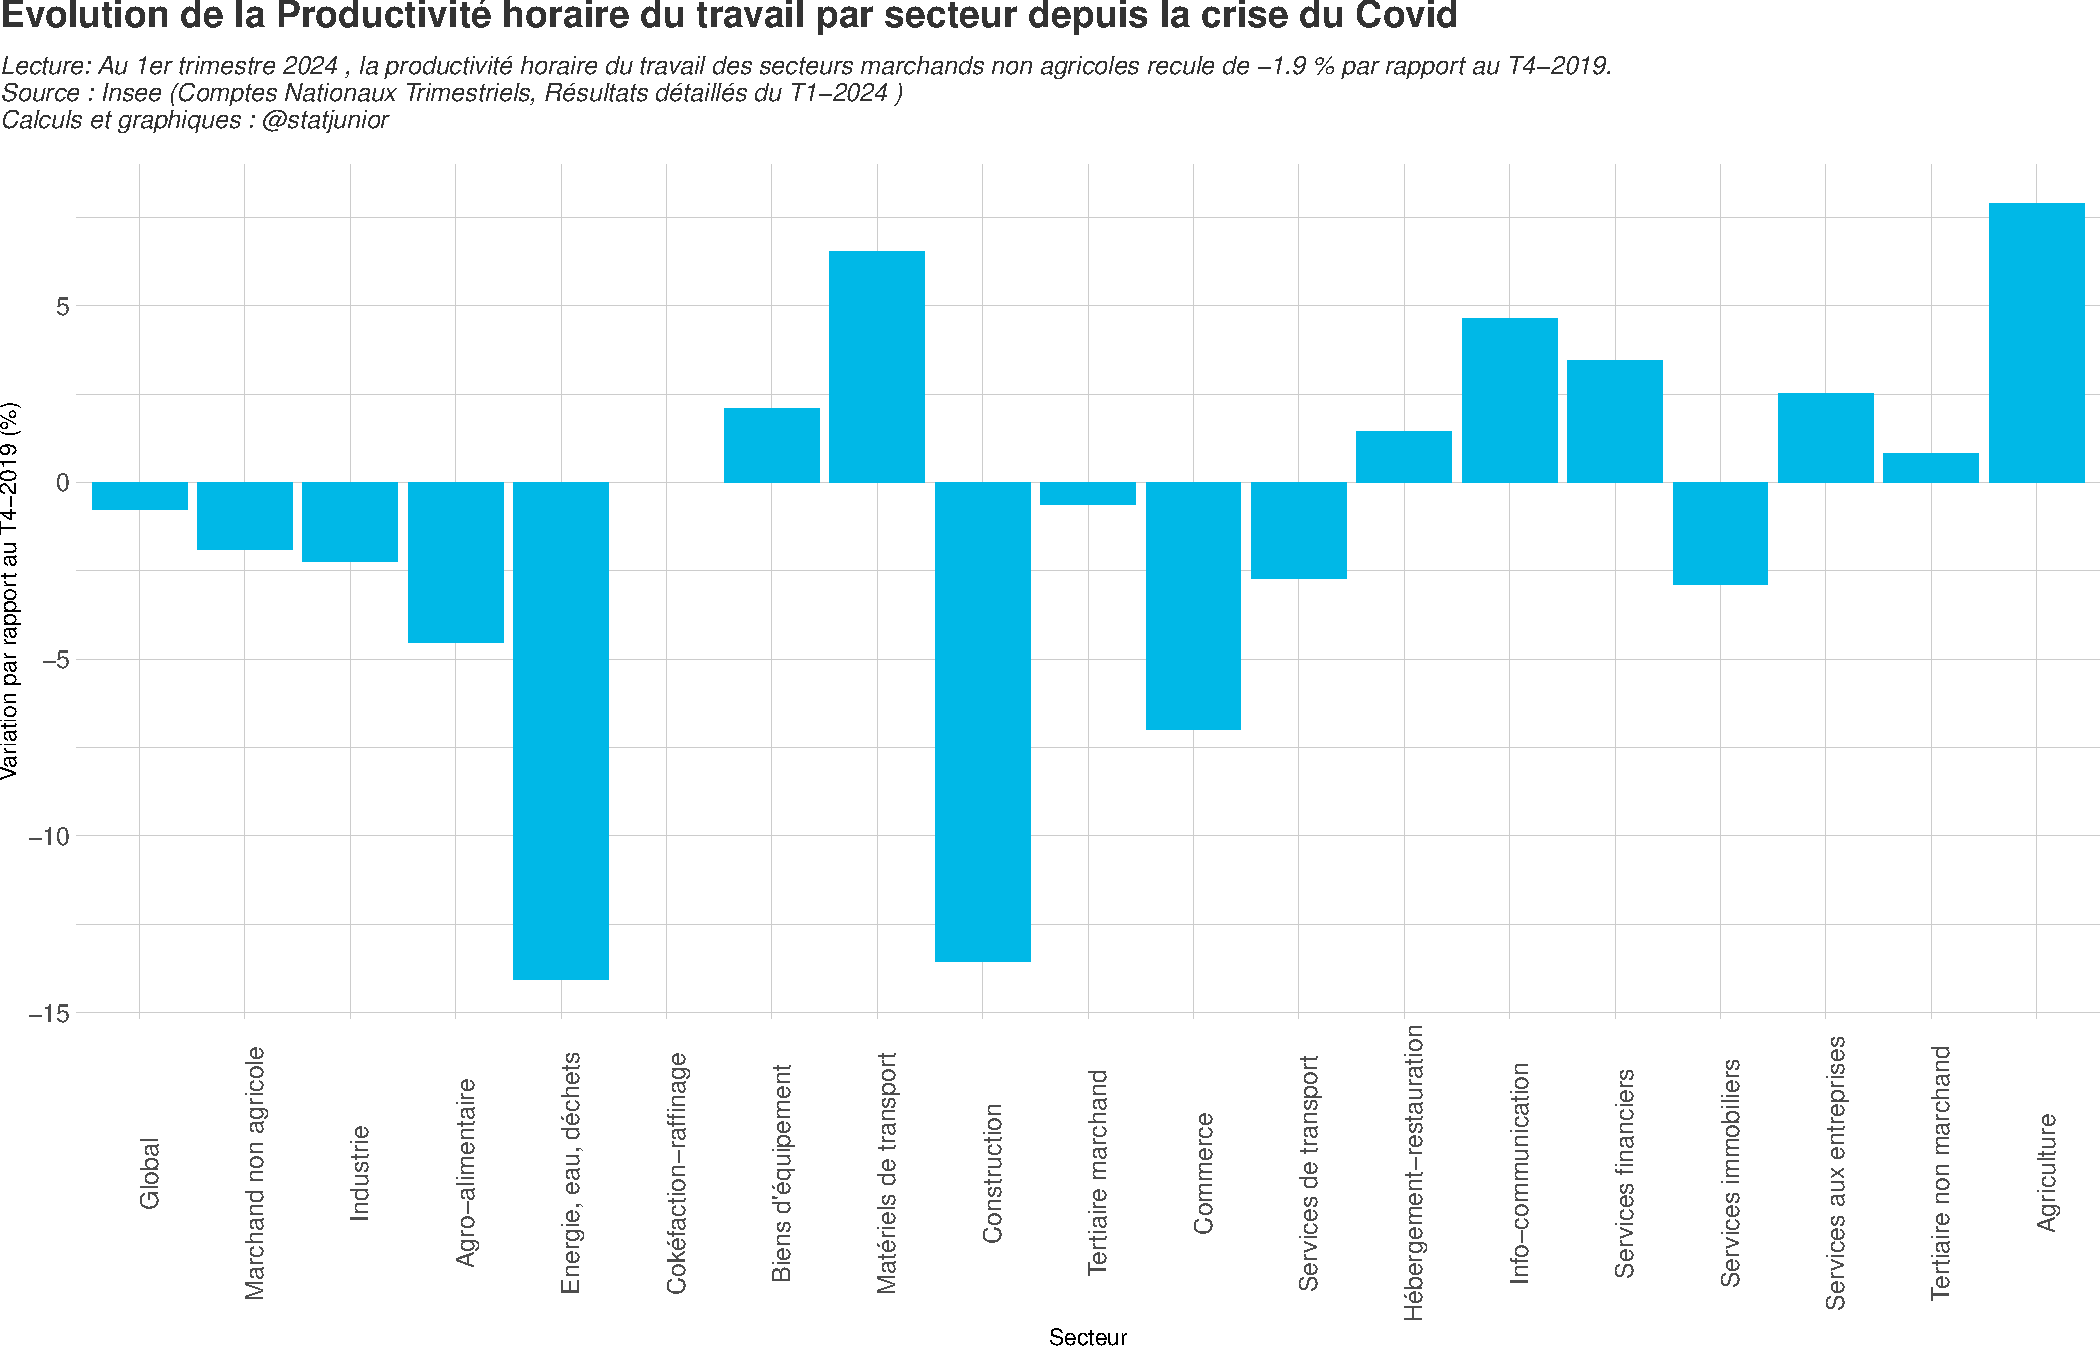
\includegraphics[keepaspectratio]{rapport_pdf_compte_branche_files/figure-latex/unnamed-chunk-26-1.pdf}}

\subsection{Evolution du volume d'heures travaillées par branche depuis
2019}\label{evolution-du-volume-dheures-travailluxe9es-par-branche-depuis-2019}

\pandocbounded{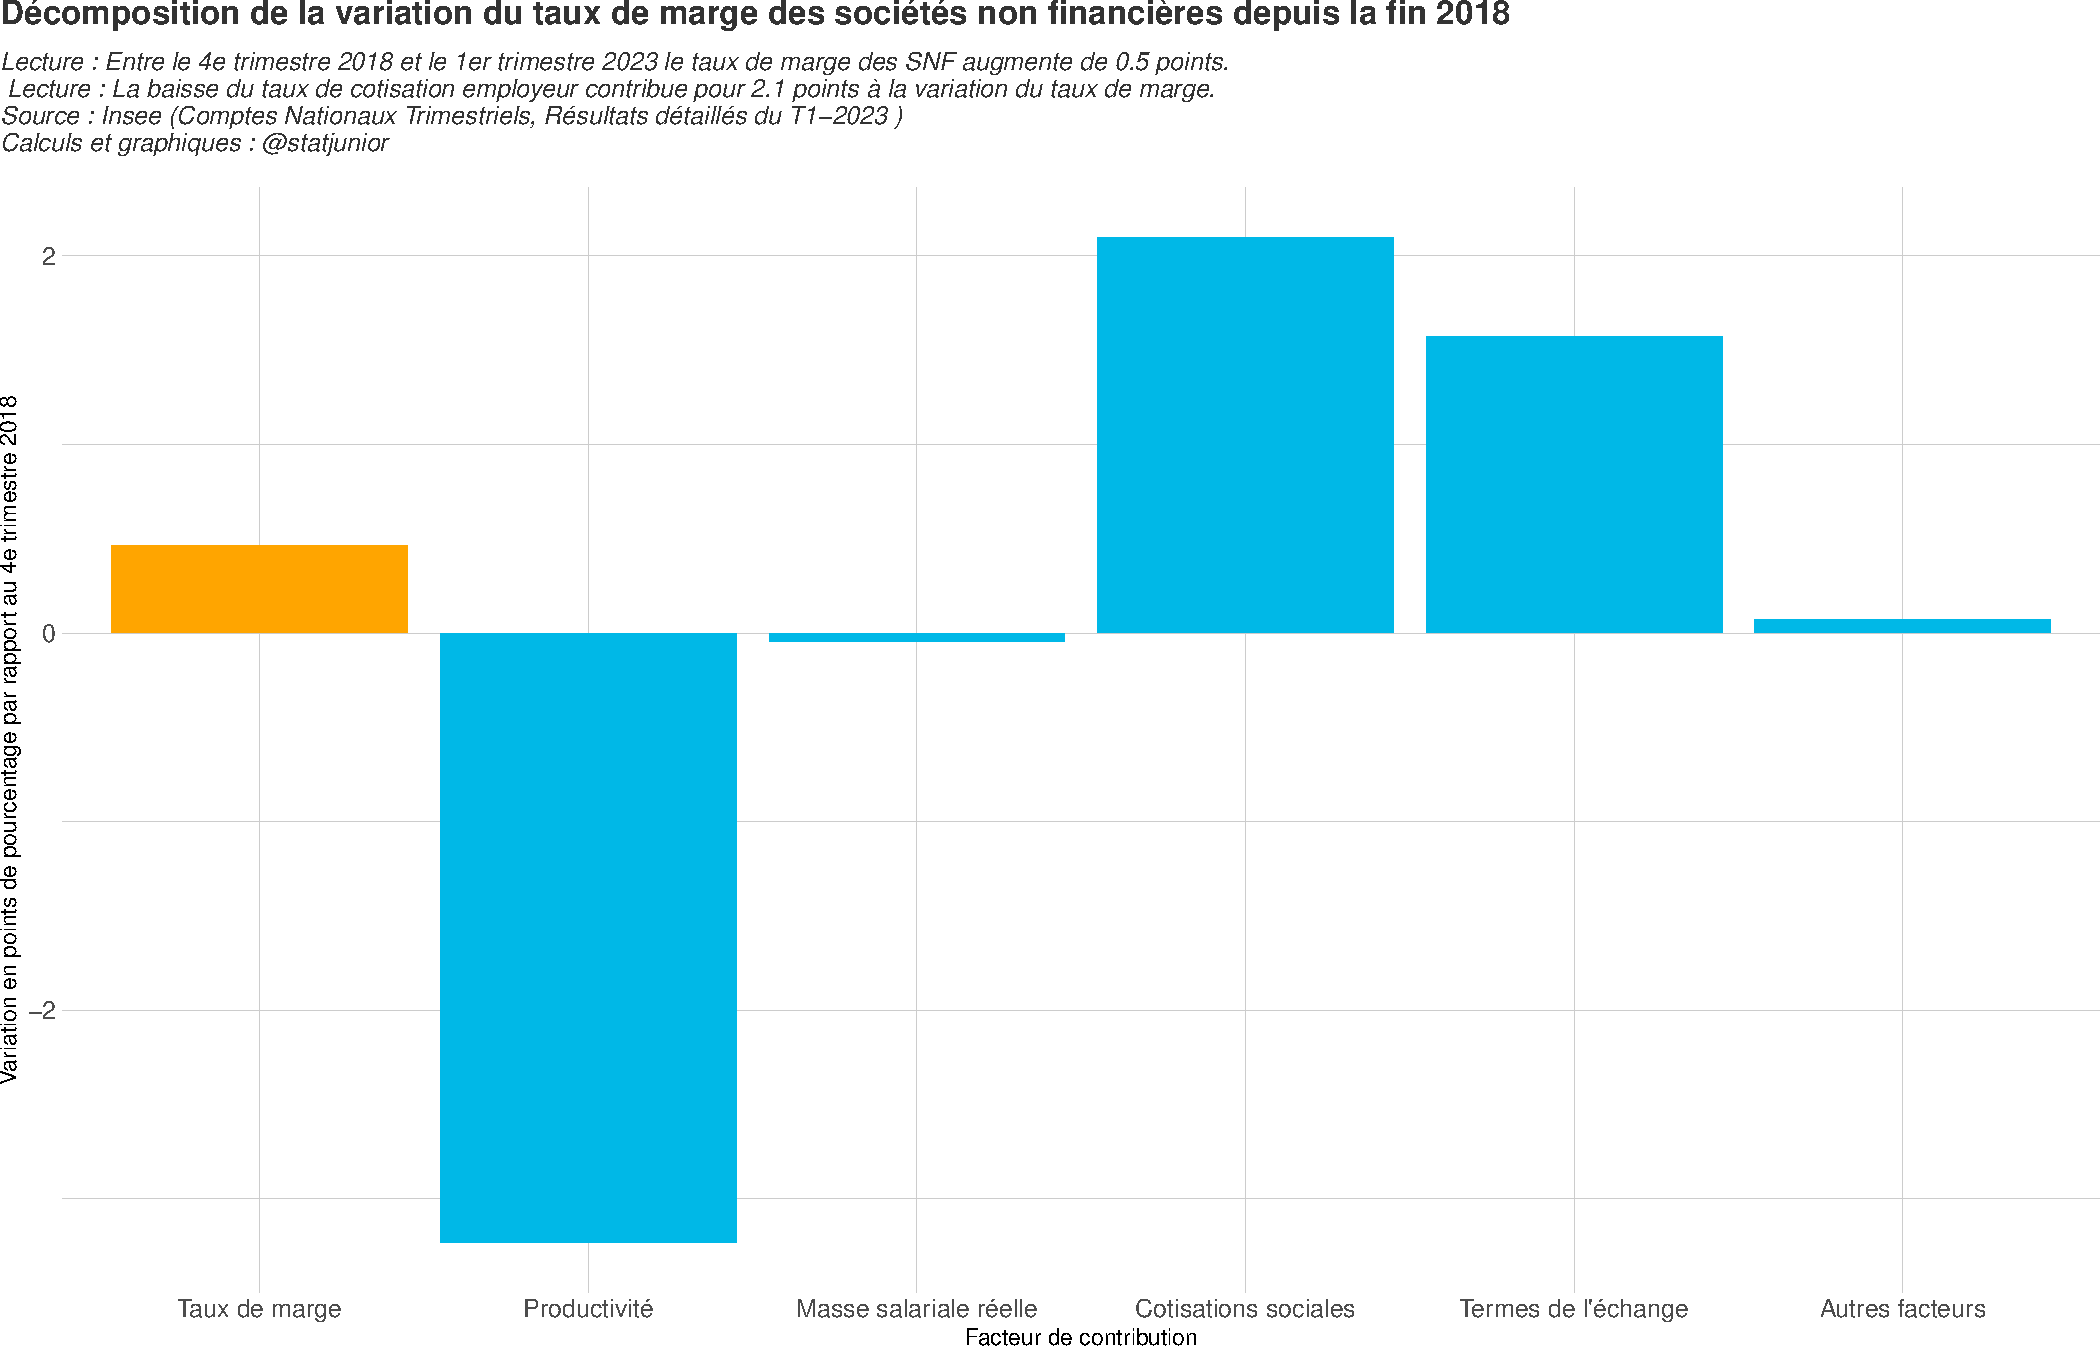
\includegraphics[keepaspectratio]{rapport_pdf_compte_branche_files/figure-latex/unnamed-chunk-27-1.pdf}}

\subsection{Décomposition de la Productivité : contribution de la valeur
ajoutée et du volume d'heures travaillées par
secteur}\label{duxe9composition-de-la-productivituxe9-contribution-de-la-valeur-ajoutuxe9e-et-du-volume-dheures-travailluxe9es-par-secteur}

\pandocbounded{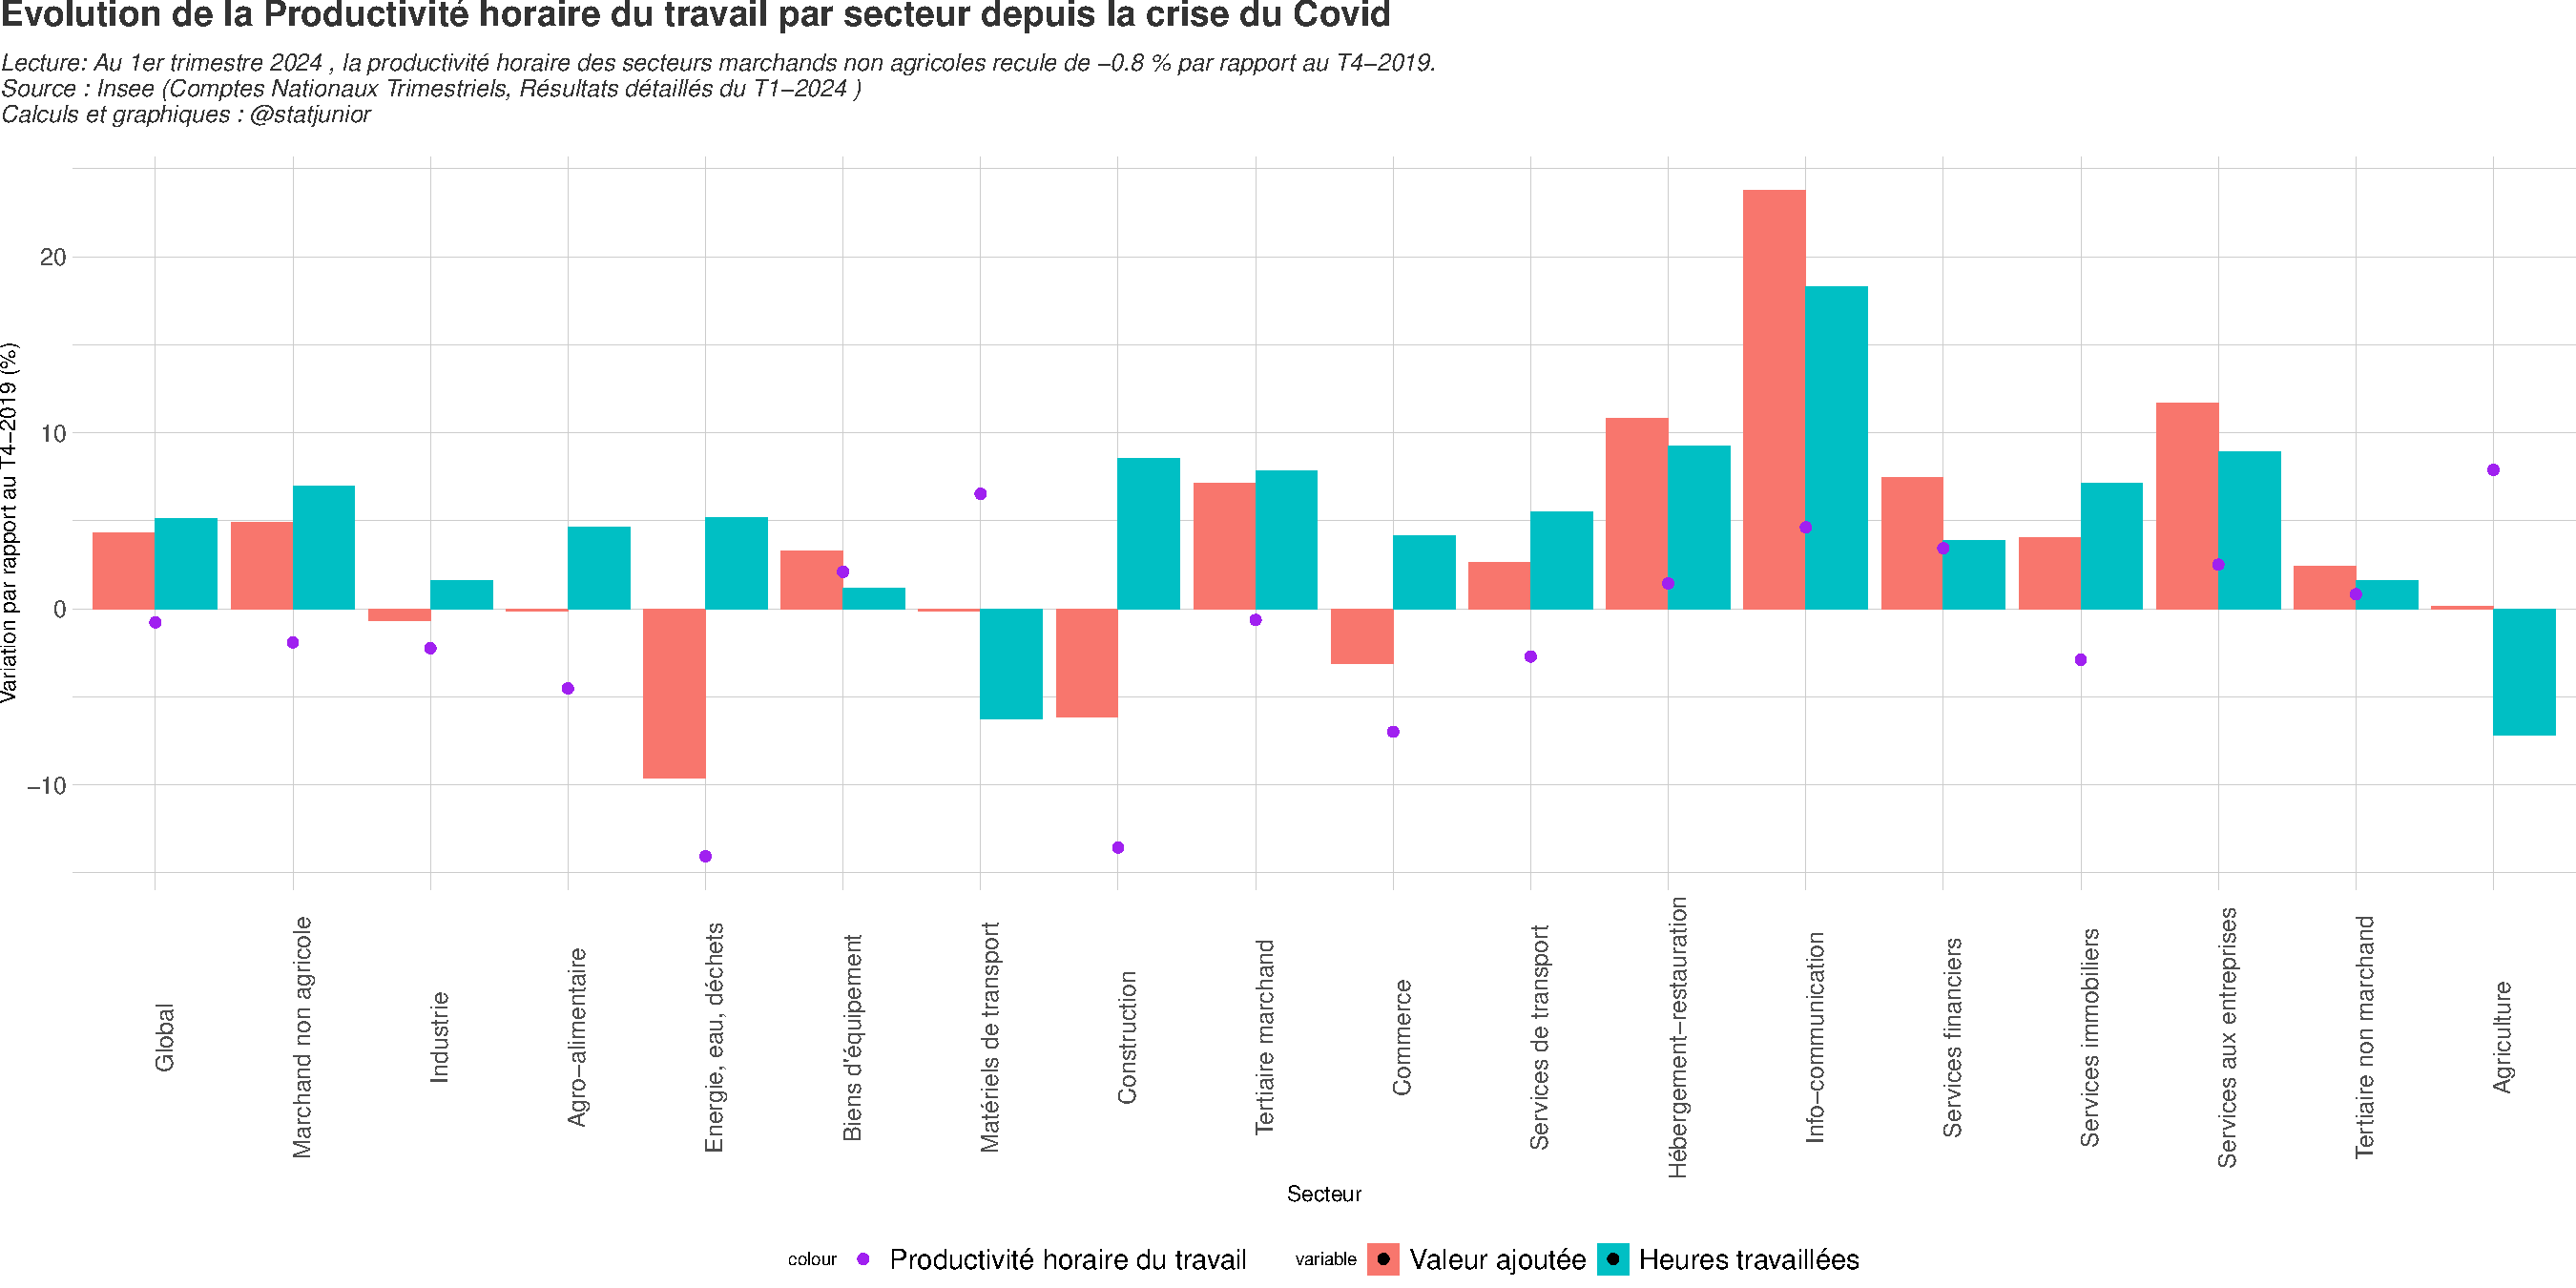
\includegraphics[keepaspectratio]{rapport_pdf_compte_branche_files/figure-latex/unnamed-chunk-28-1.pdf}}

\newpage

\section{Taux de marge}\label{taux-de-marge}

\subsection{Evolution du taux de marge sur longue
période}\label{evolution-du-taux-de-marge-sur-longue-puxe9riode}

\pandocbounded{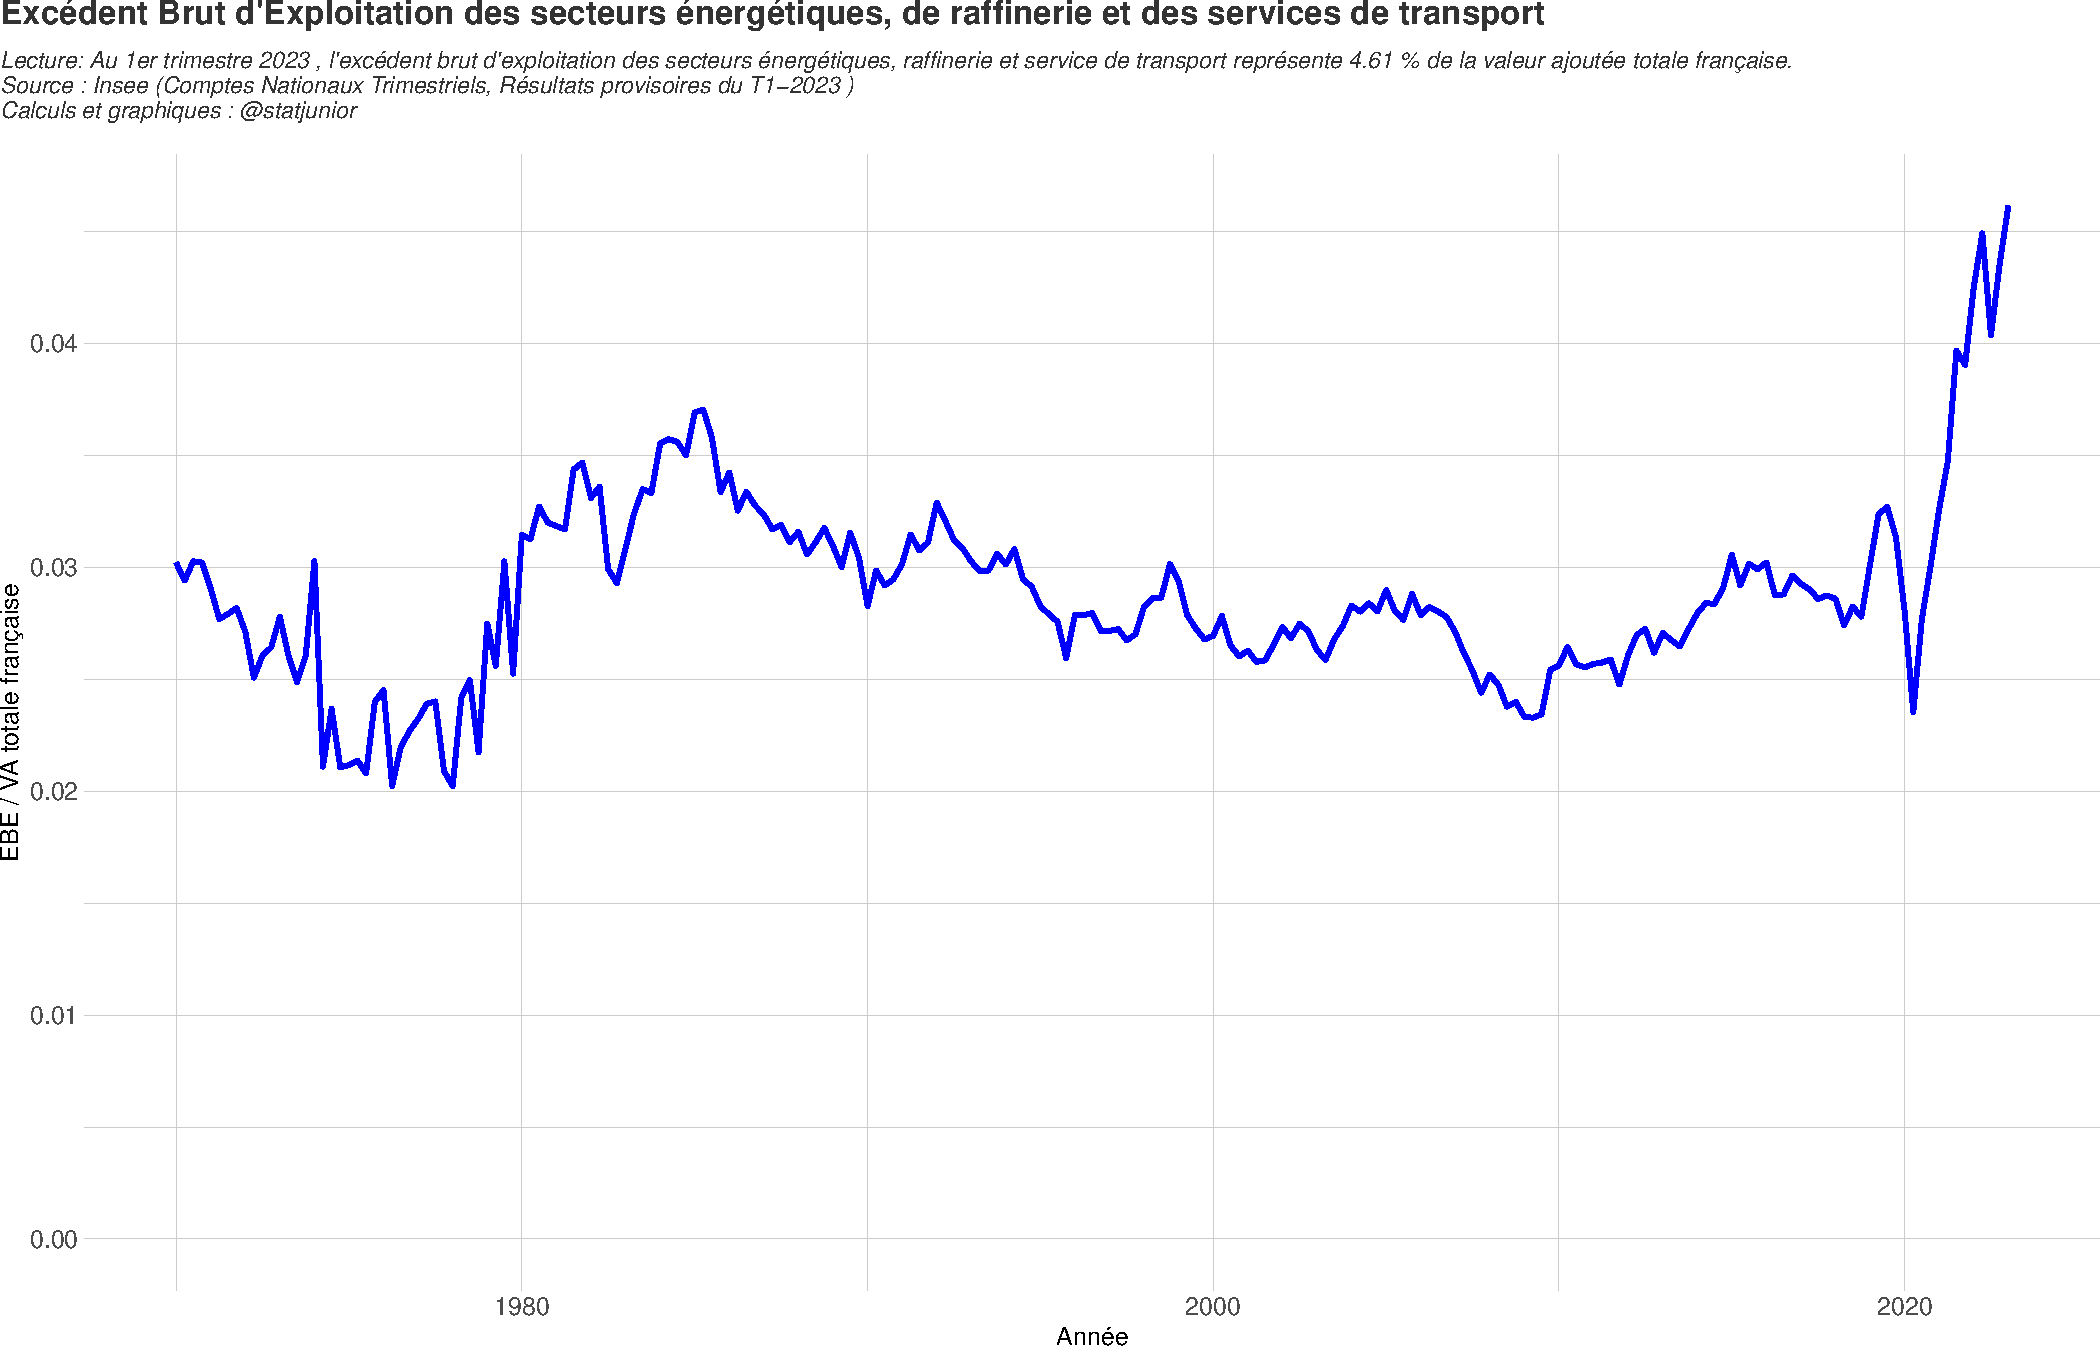
\includegraphics[keepaspectratio]{rapport_pdf_compte_branche_files/figure-latex/unnamed-chunk-29-1.pdf}}

\subsection{Evolution du taux de marge par secteur par rapport à l'année
2019}\label{evolution-du-taux-de-marge-par-secteur-par-rapport-uxe0-lannuxe9e-2019}

\pandocbounded{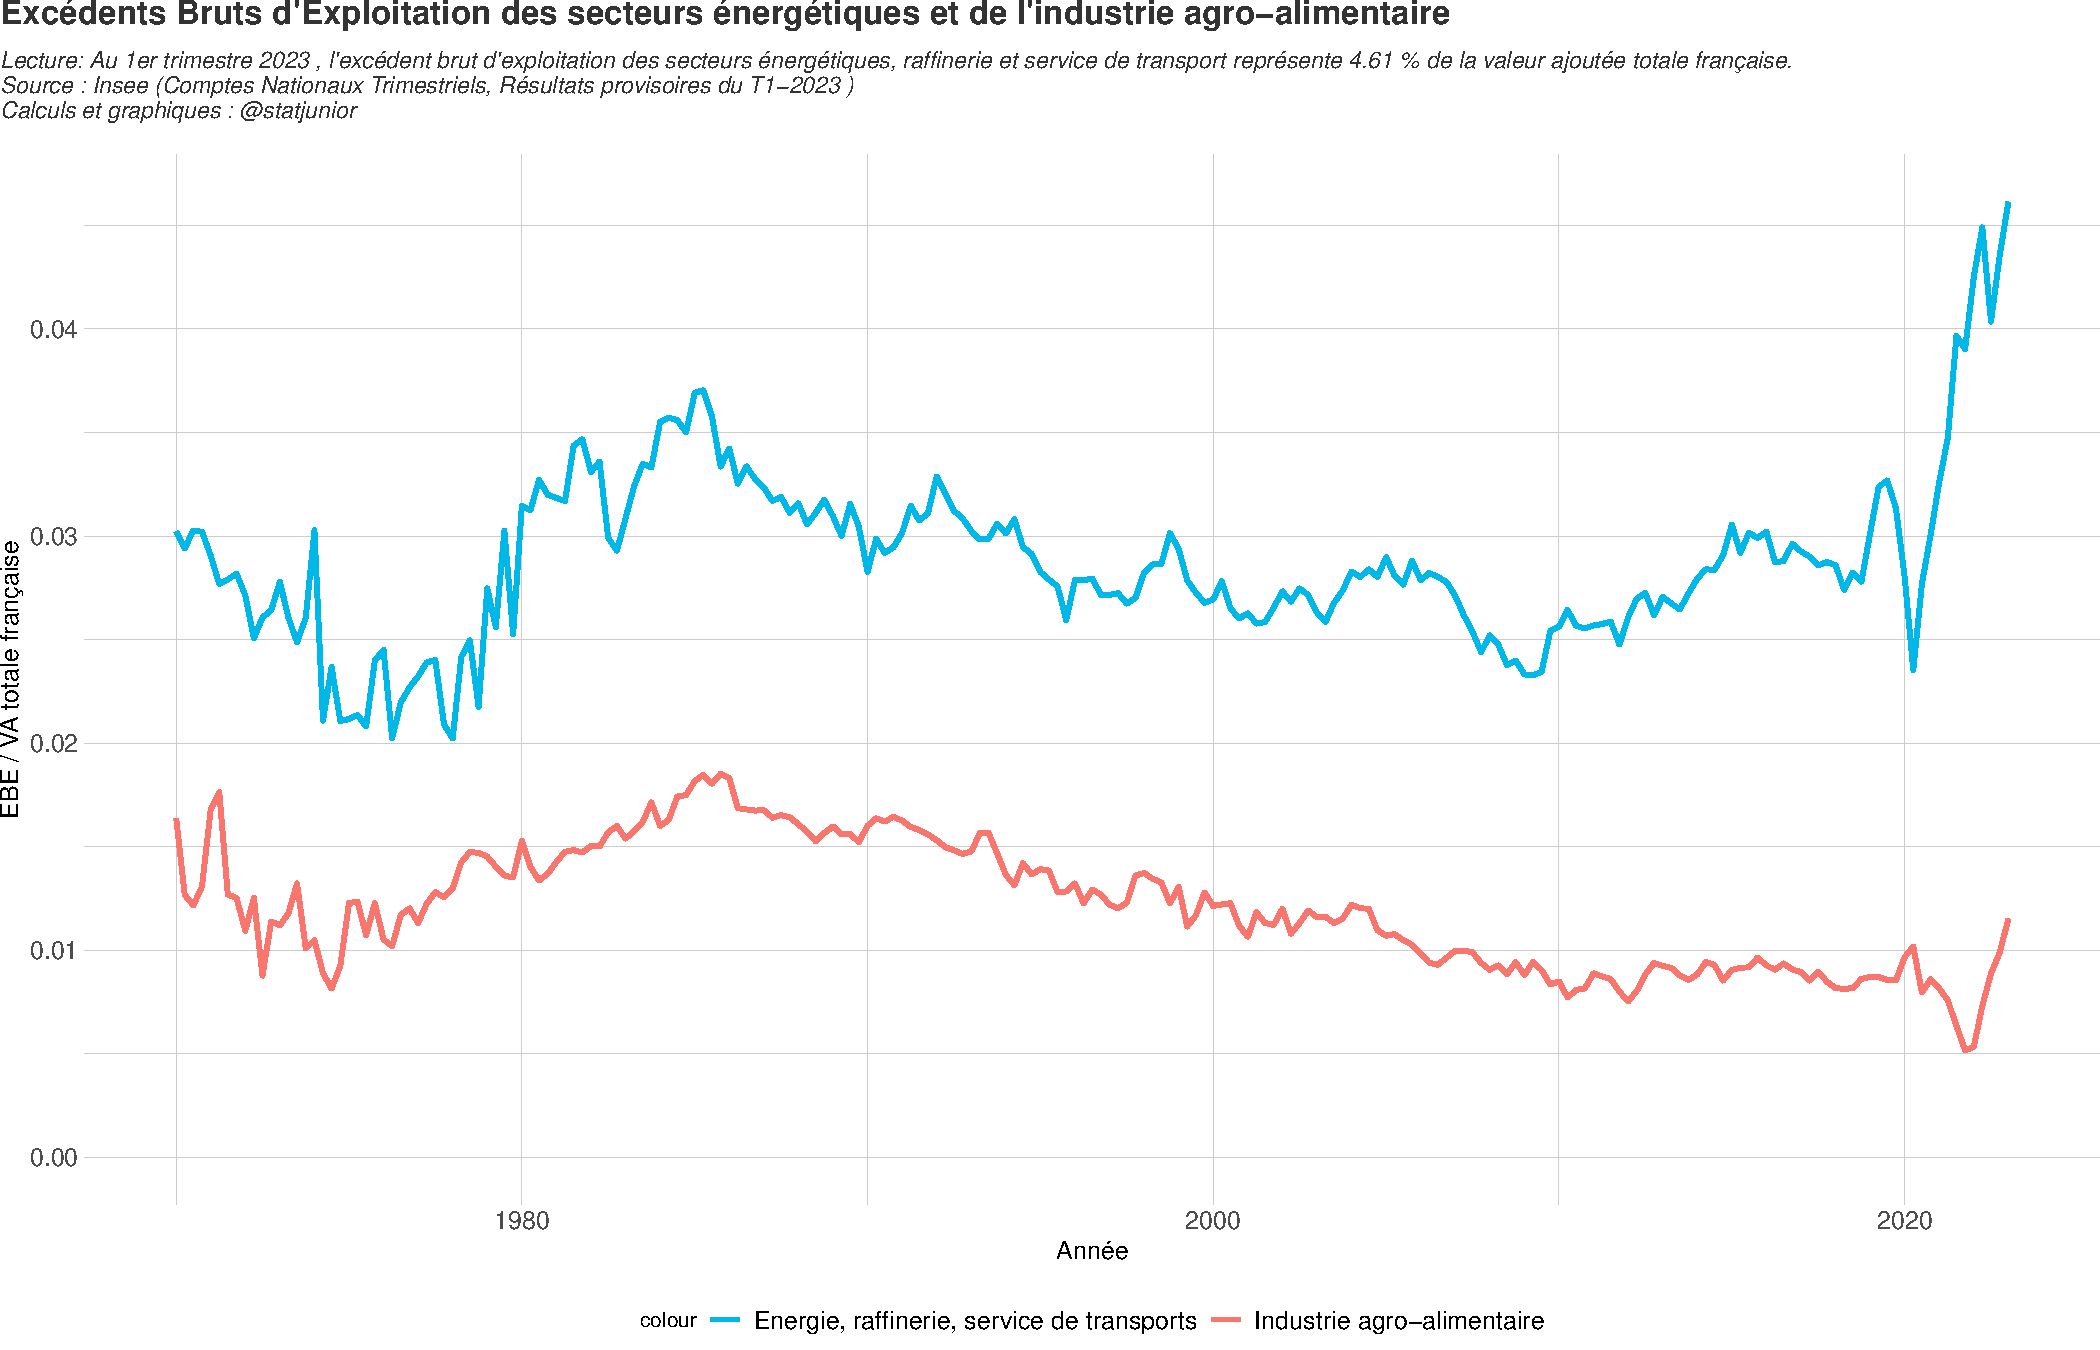
\includegraphics[keepaspectratio]{rapport_pdf_compte_branche_files/figure-latex/unnamed-chunk-30-1.pdf}}

\newpage

\section{Profits exceptionnels liés aux tensions inflationnistes depuis
2021}\label{profits-exceptionnels-liuxe9s-aux-tensions-inflationnistes-depuis-2021}

\subsection{Taux de marge des secteurs énergétiques et des services de
transport}\label{taux-de-marge-des-secteurs-uxe9nerguxe9tiques-et-des-services-de-transport}

\pandocbounded{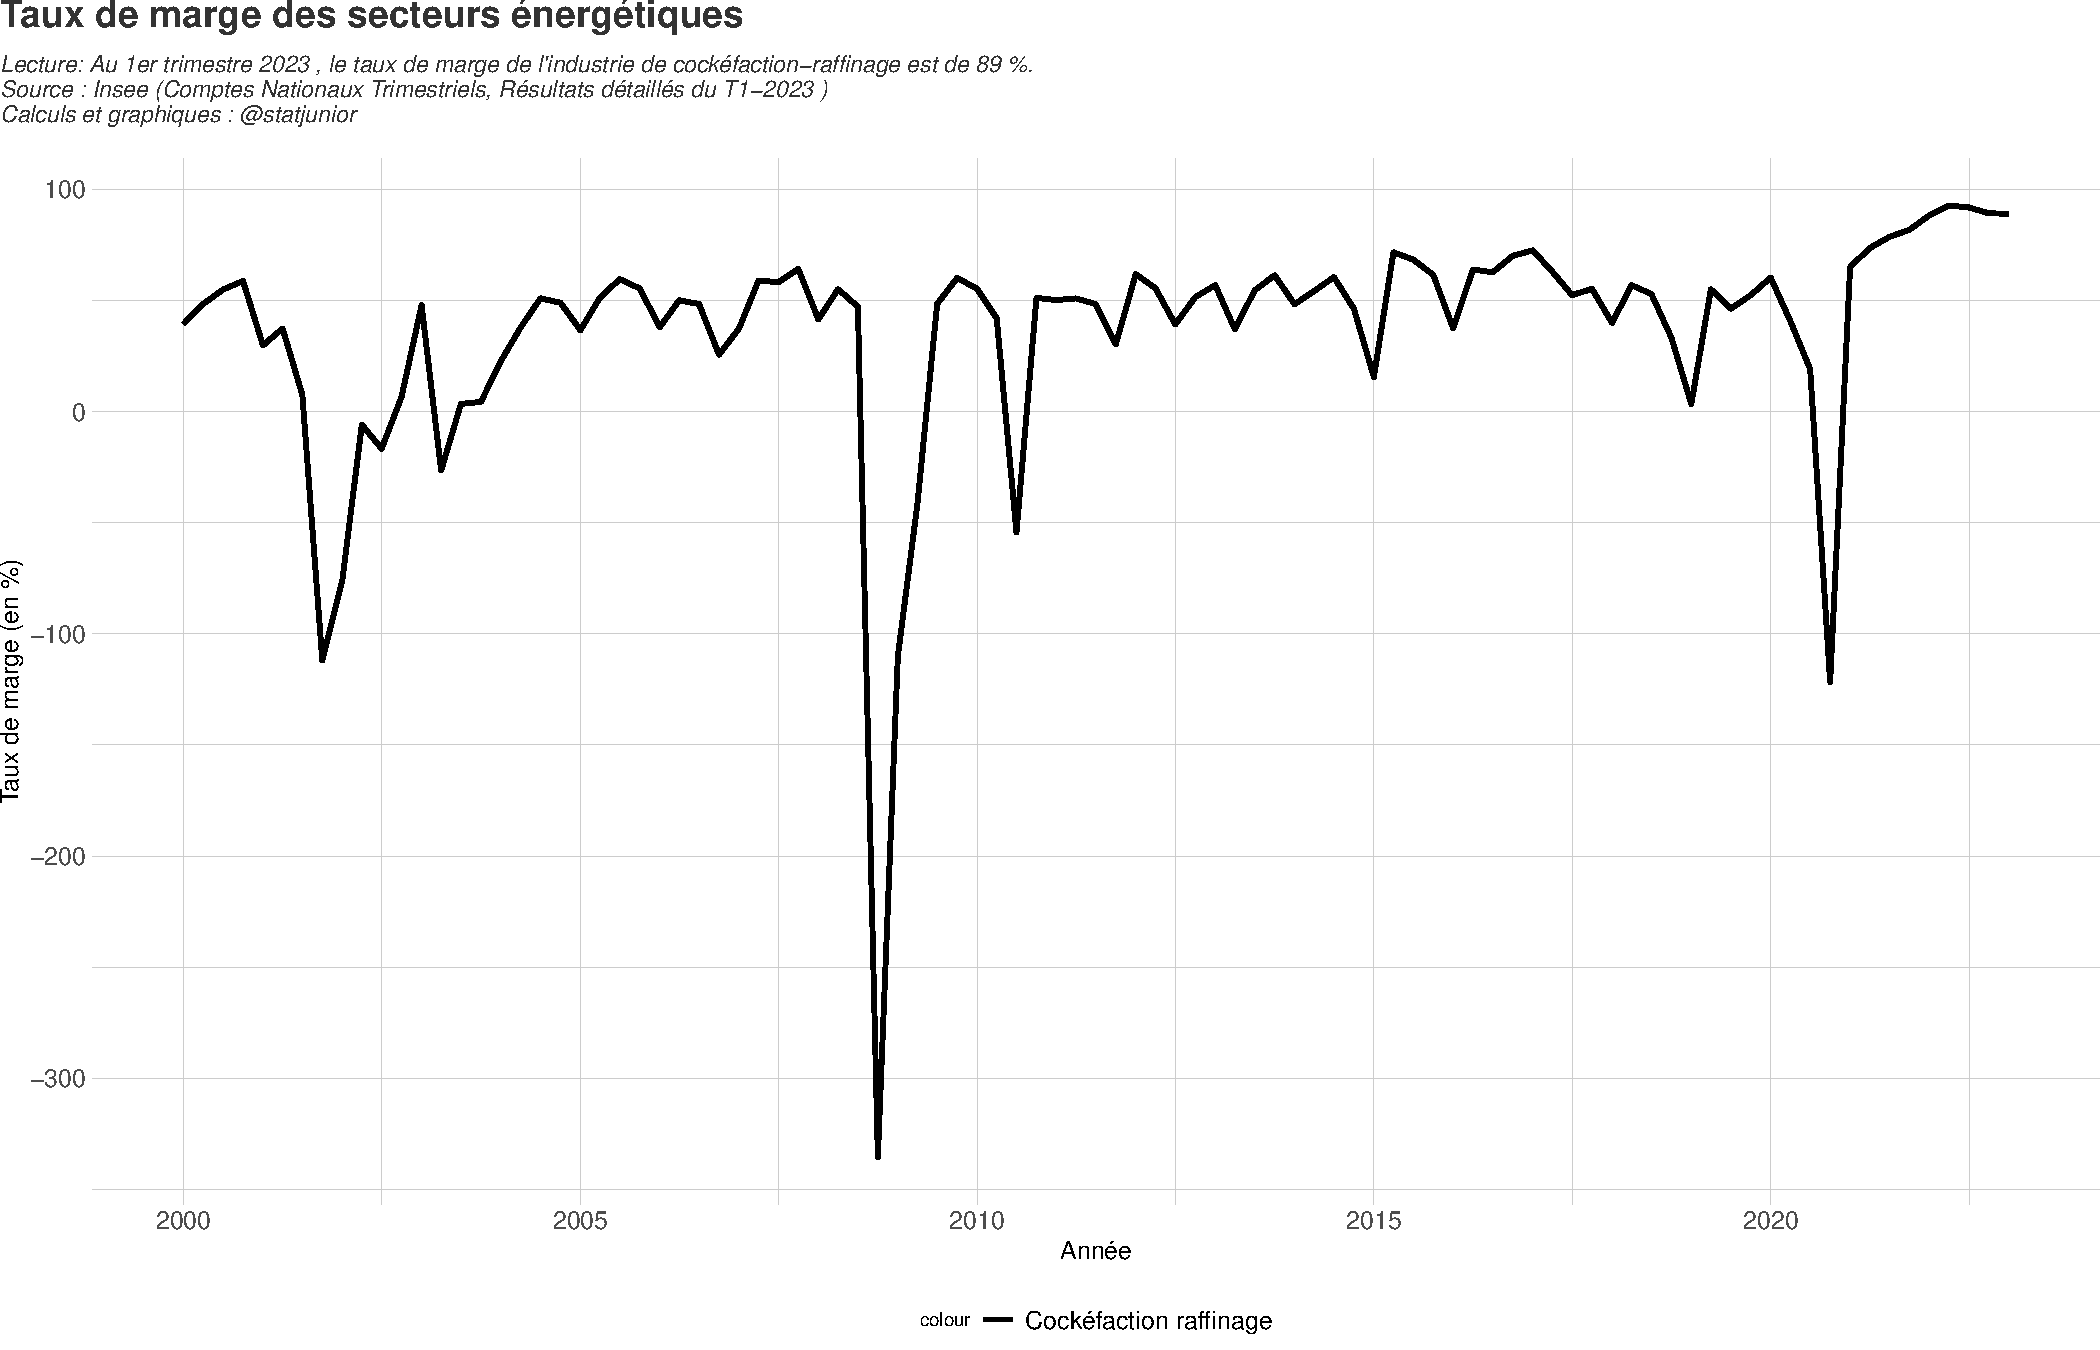
\includegraphics[keepaspectratio]{rapport_pdf_compte_branche_files/figure-latex/unnamed-chunk-32-1.pdf}}

\subsection{Taux de marge de l'industrie cockéfaction -
raffinage}\label{taux-de-marge-de-lindustrie-cockuxe9faction---raffinage}

\subsection{Taux de marge de l'industrie
agro-alimentaire}\label{taux-de-marge-de-lindustrie-agro-alimentaire}

\pandocbounded{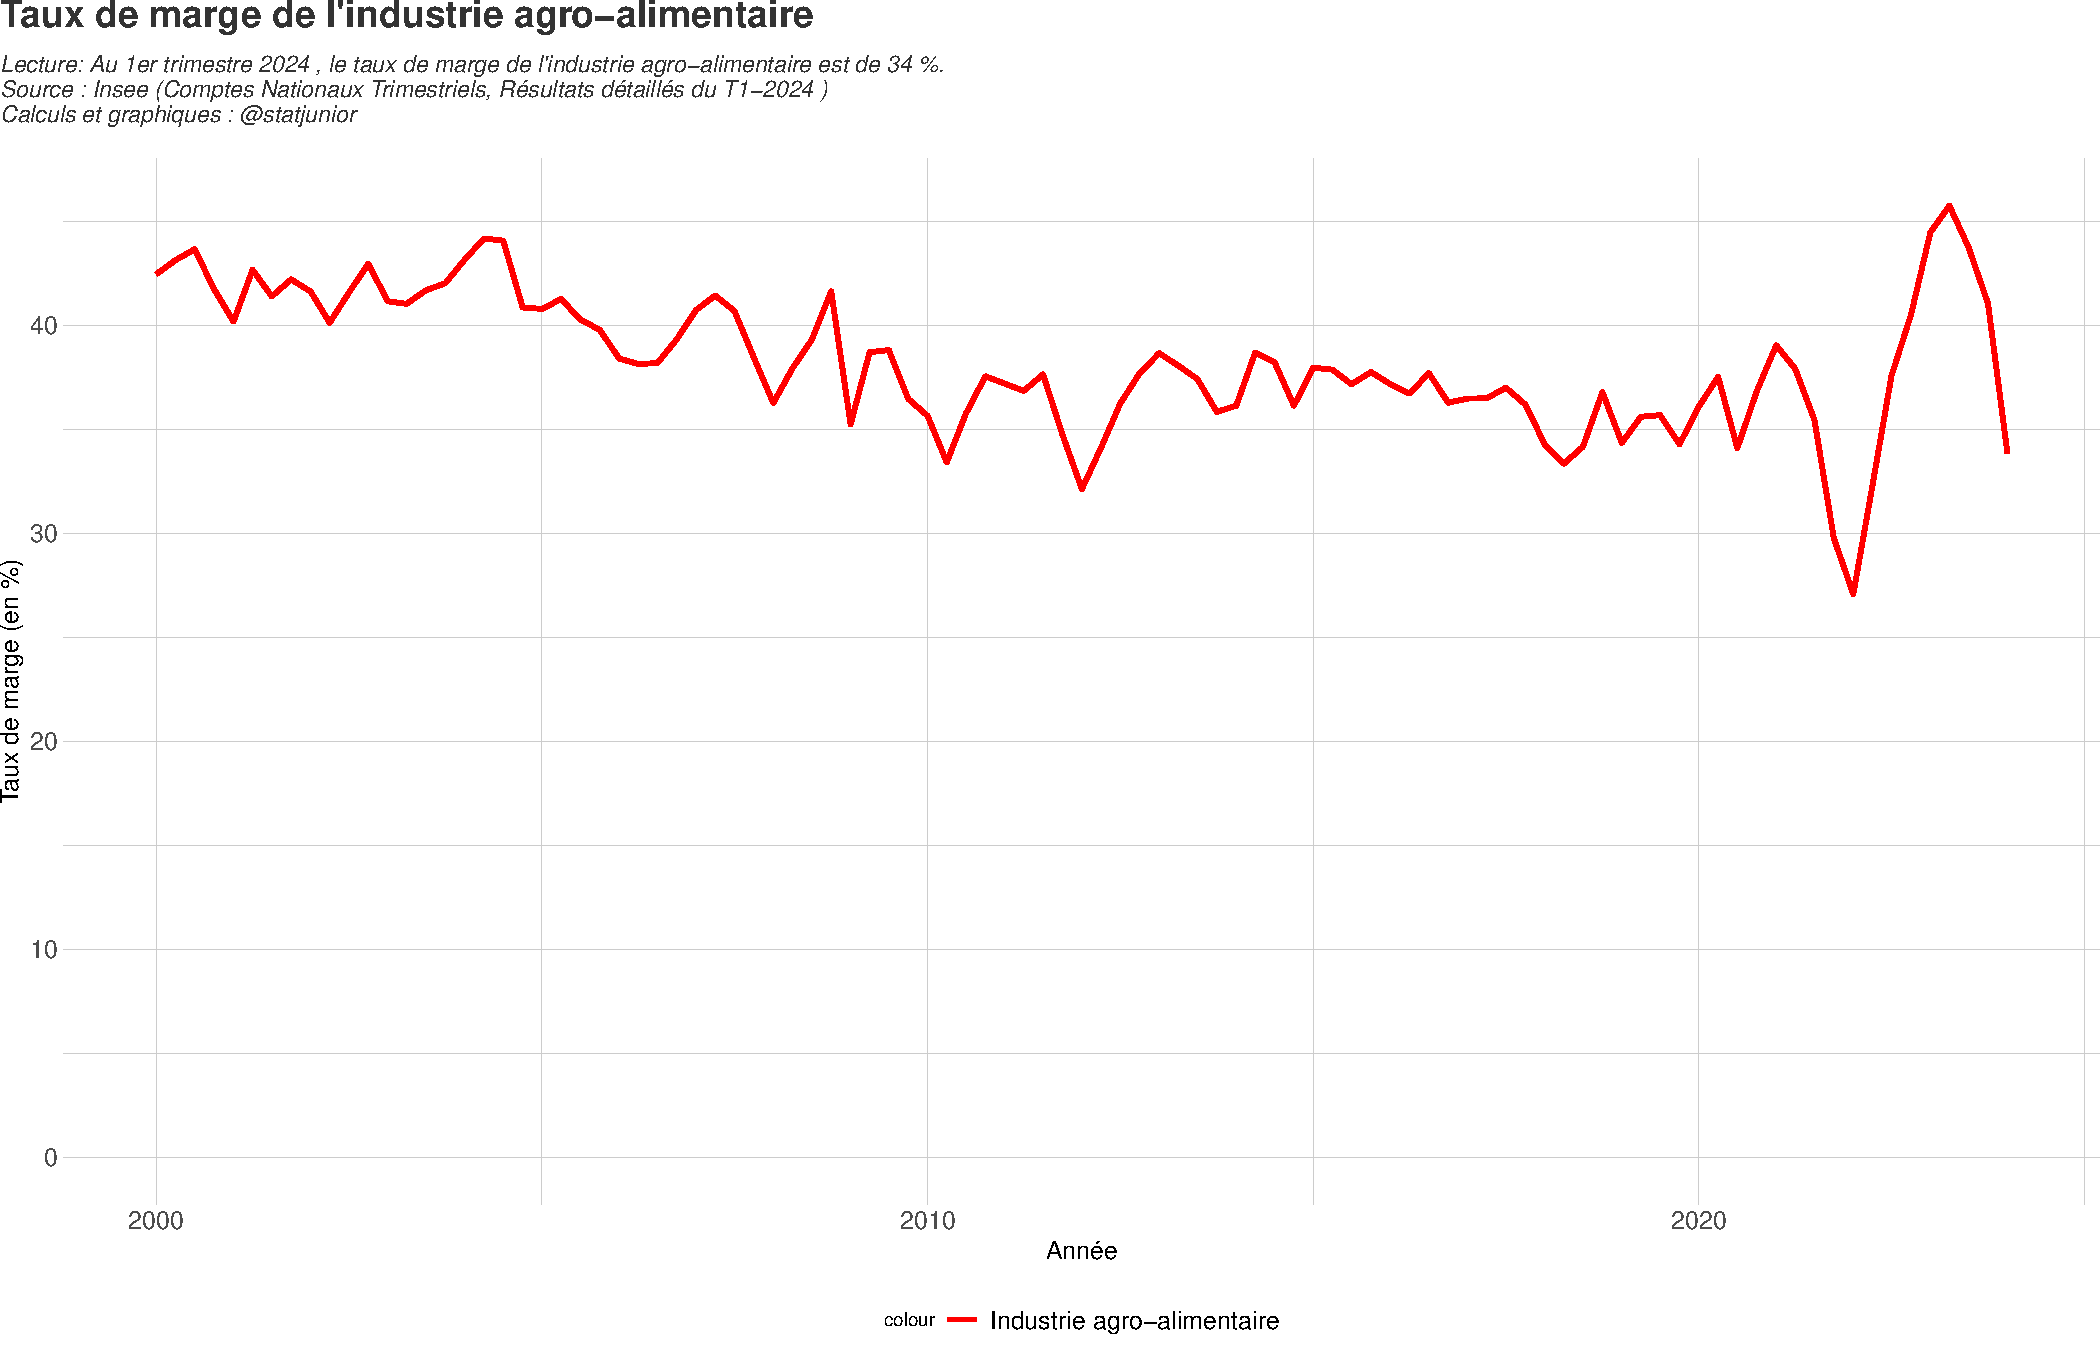
\includegraphics[keepaspectratio]{rapport_pdf_compte_branche_files/figure-latex/unnamed-chunk-35-1.pdf}}

\subsection{Part des profits exceptionnels des secteurs énergétiques
dans l'ensemble de la valeur ajoutée
française}\label{part-des-profits-exceptionnels-des-secteurs-uxe9nerguxe9tiques-dans-lensemble-de-la-valeur-ajoutuxe9e-franuxe7aise}

\pandocbounded{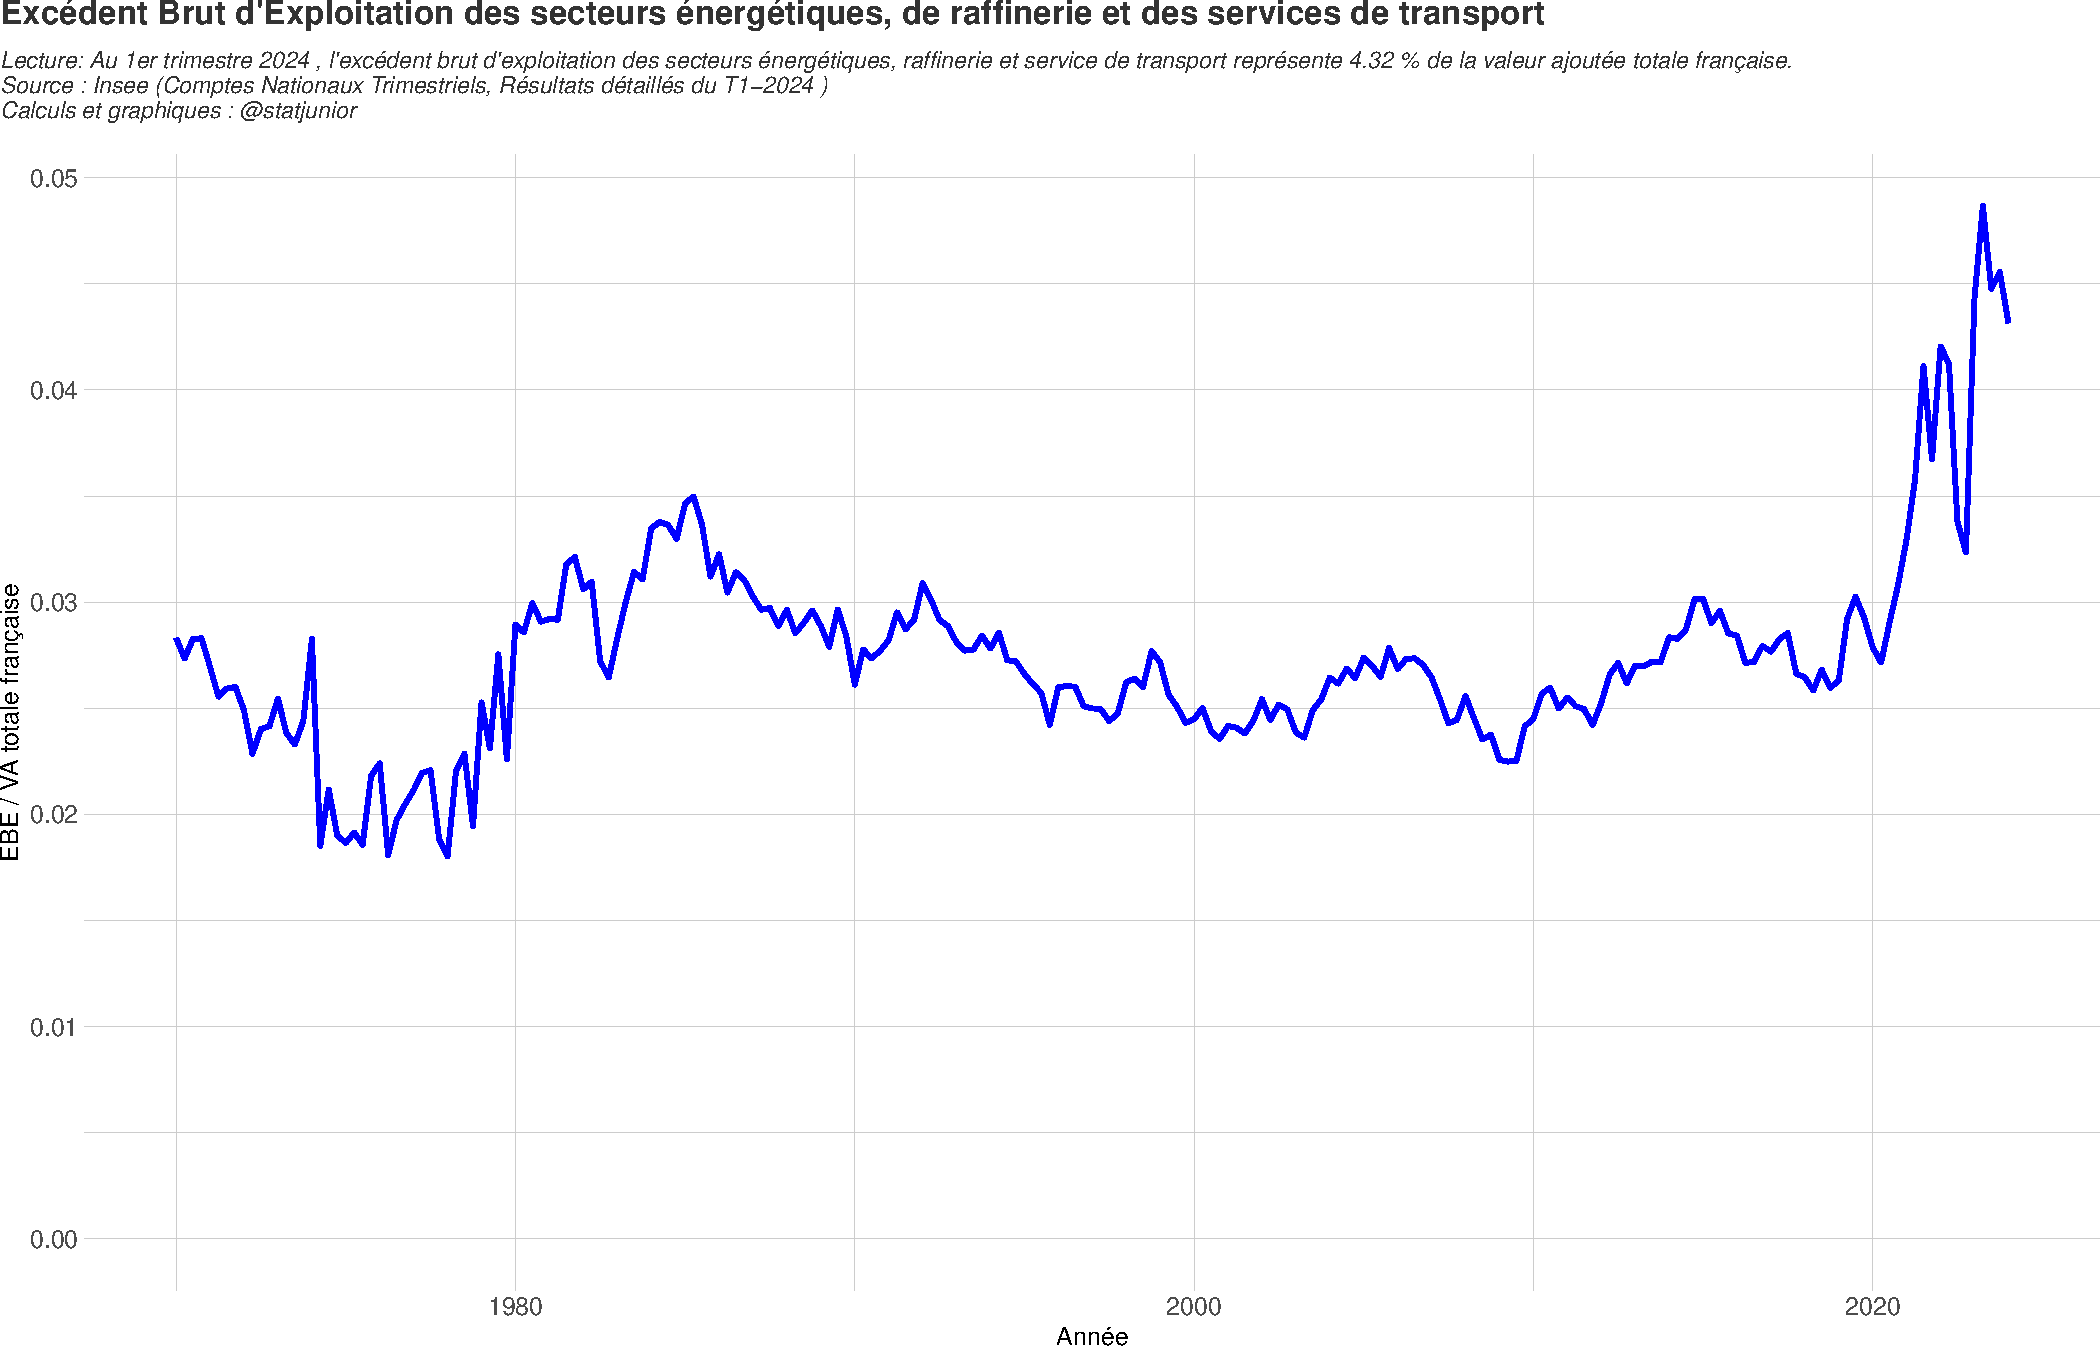
\includegraphics[keepaspectratio]{rapport_pdf_compte_branche_files/figure-latex/unnamed-chunk-36-1.pdf}}

\subsection{Part des profits exceptionnels des secteurs énergétiques et
de l'industrie agro-alimentaire dans l'économie
française}\label{part-des-profits-exceptionnels-des-secteurs-uxe9nerguxe9tiques-et-de-lindustrie-agro-alimentaire-dans-luxe9conomie-franuxe7aise}

\pandocbounded{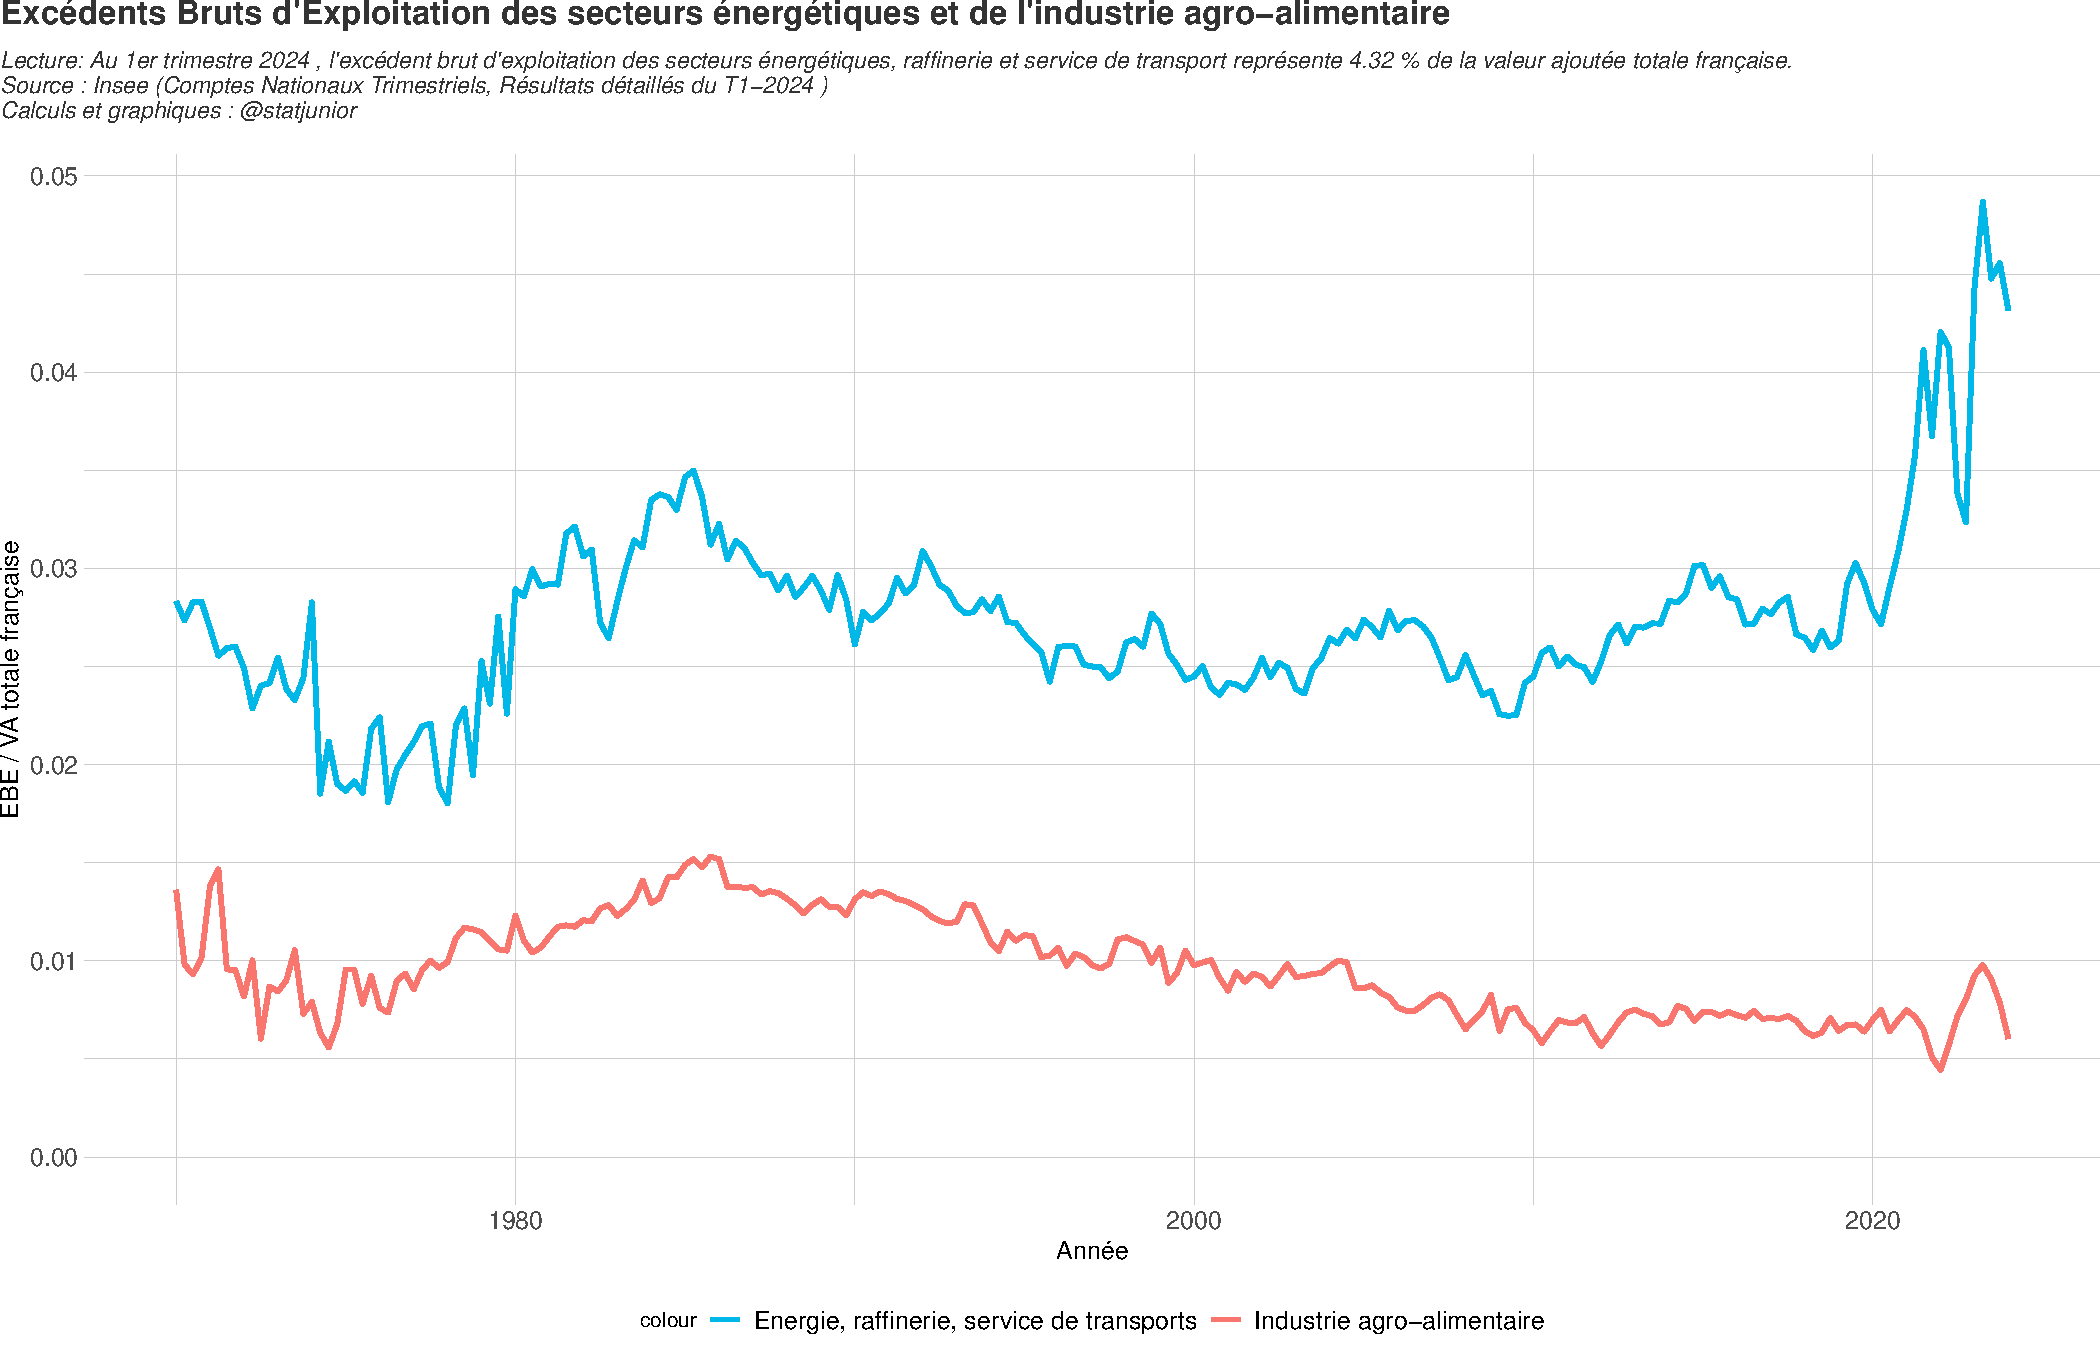
\includegraphics[keepaspectratio]{rapport_pdf_compte_branche_files/figure-latex/unnamed-chunk-37-1.pdf}}

\section{Partage de la valeur ajoutée entre salaires et
profits}\label{partage-de-la-valeur-ajoutuxe9e-entre-salaires-et-profits}

\subsection{Masse salariale et Excédent brut d'exploitation depuis
2018}\label{masse-salariale-et-excuxe9dent-brut-dexploitation-depuis-2018}

\pandocbounded{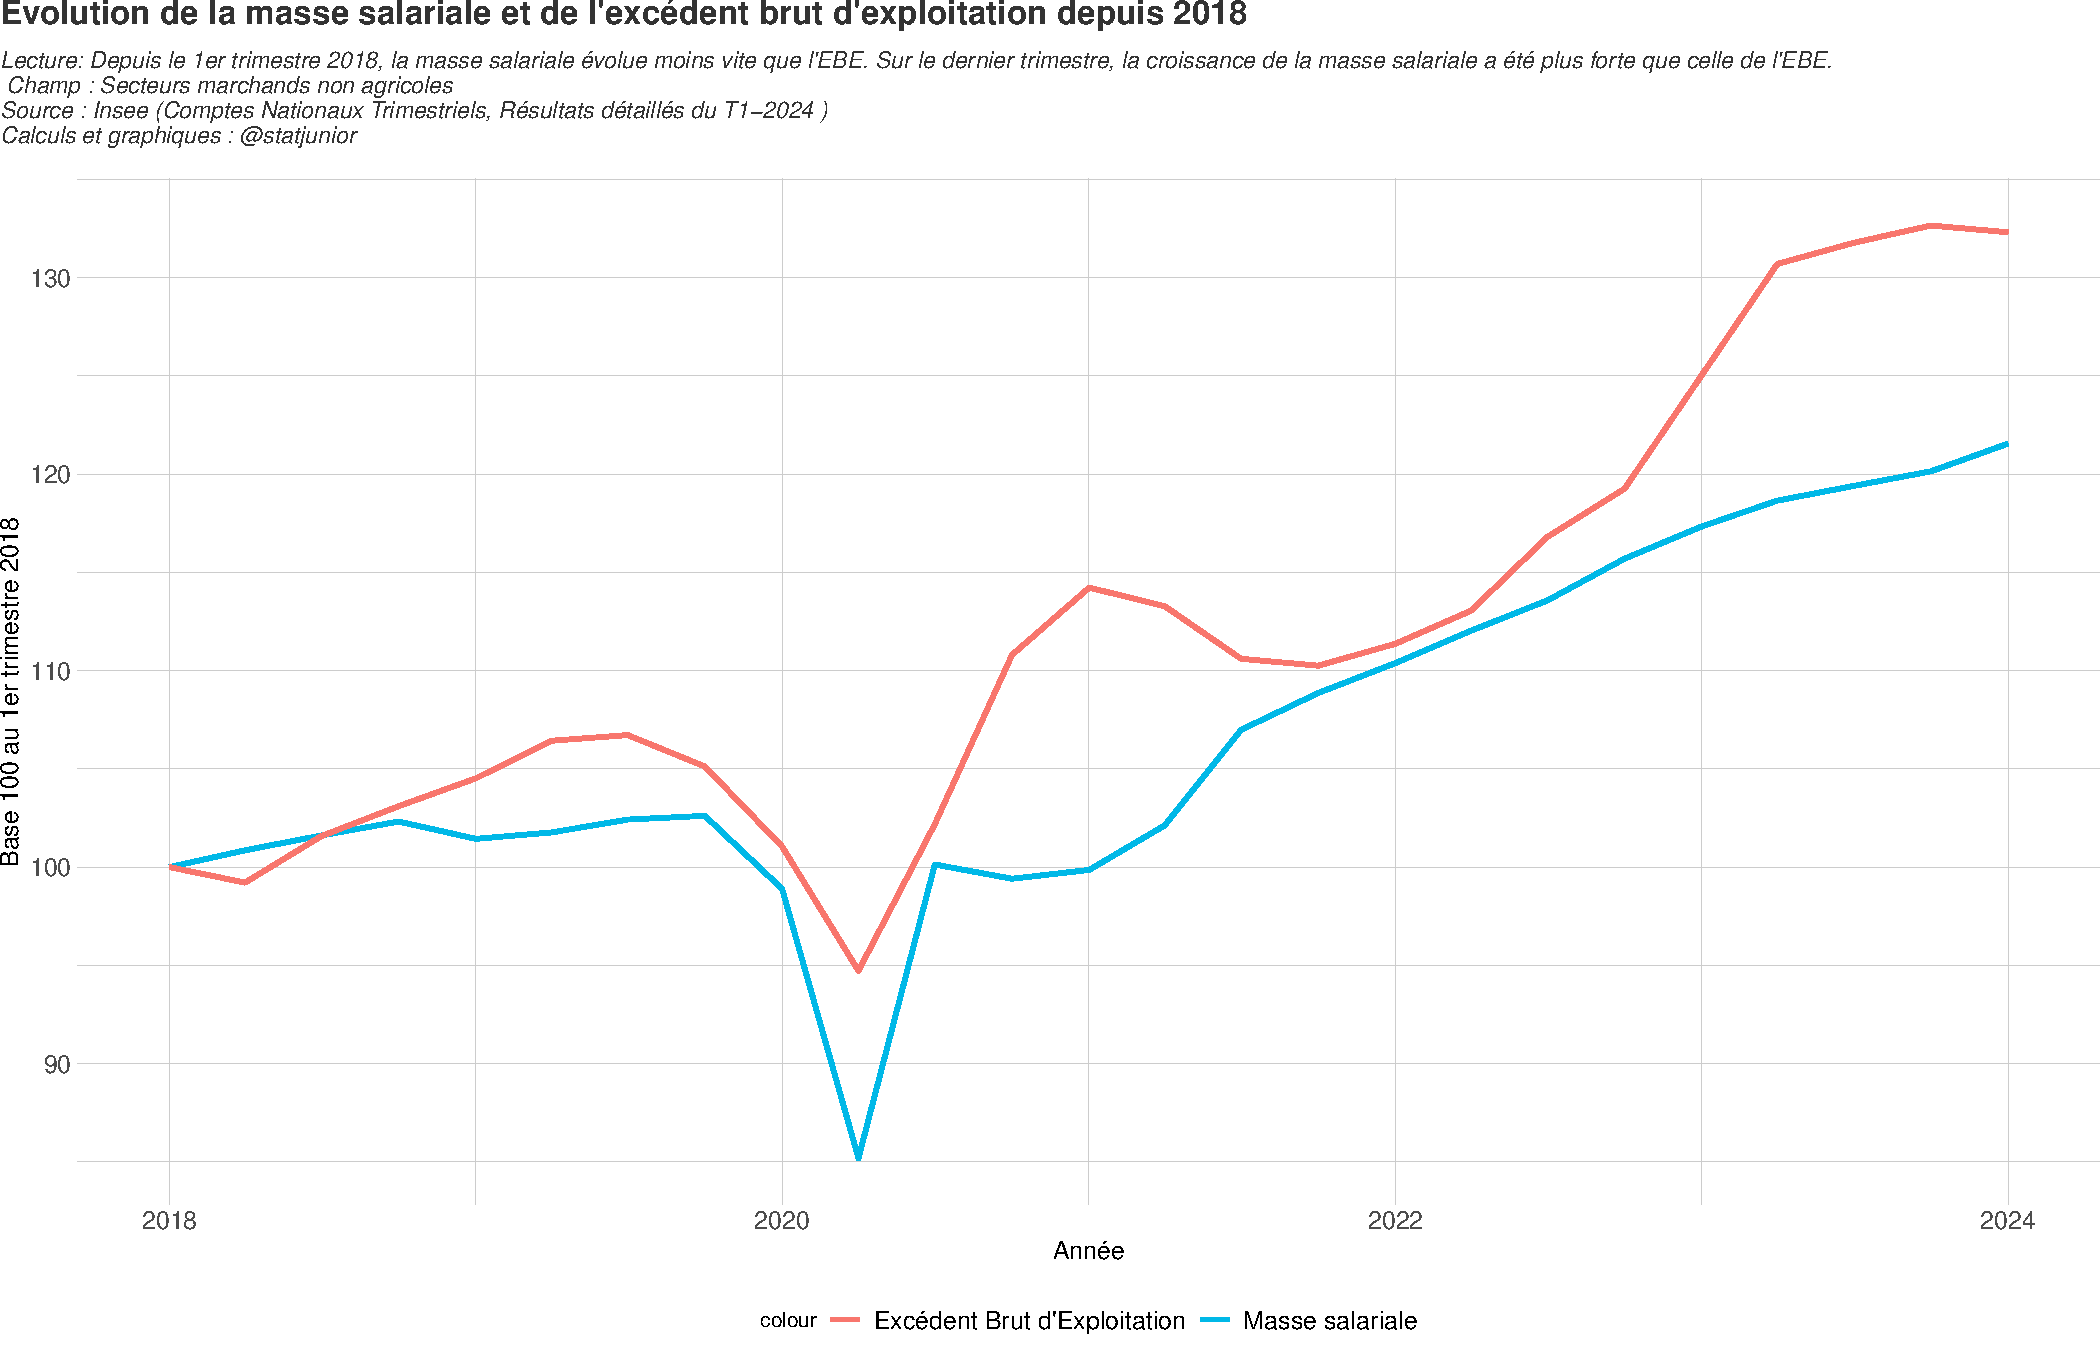
\includegraphics[keepaspectratio]{rapport_pdf_compte_branche_files/figure-latex/unnamed-chunk-40-1.pdf}}

\subsection{Evolution des coûts salariaux et des marges bénéficiaires
des entreprises depuis
2010}\label{evolution-des-couxfbts-salariaux-et-des-marges-buxe9nuxe9ficiaires-des-entreprises-depuis-2010}

\pandocbounded{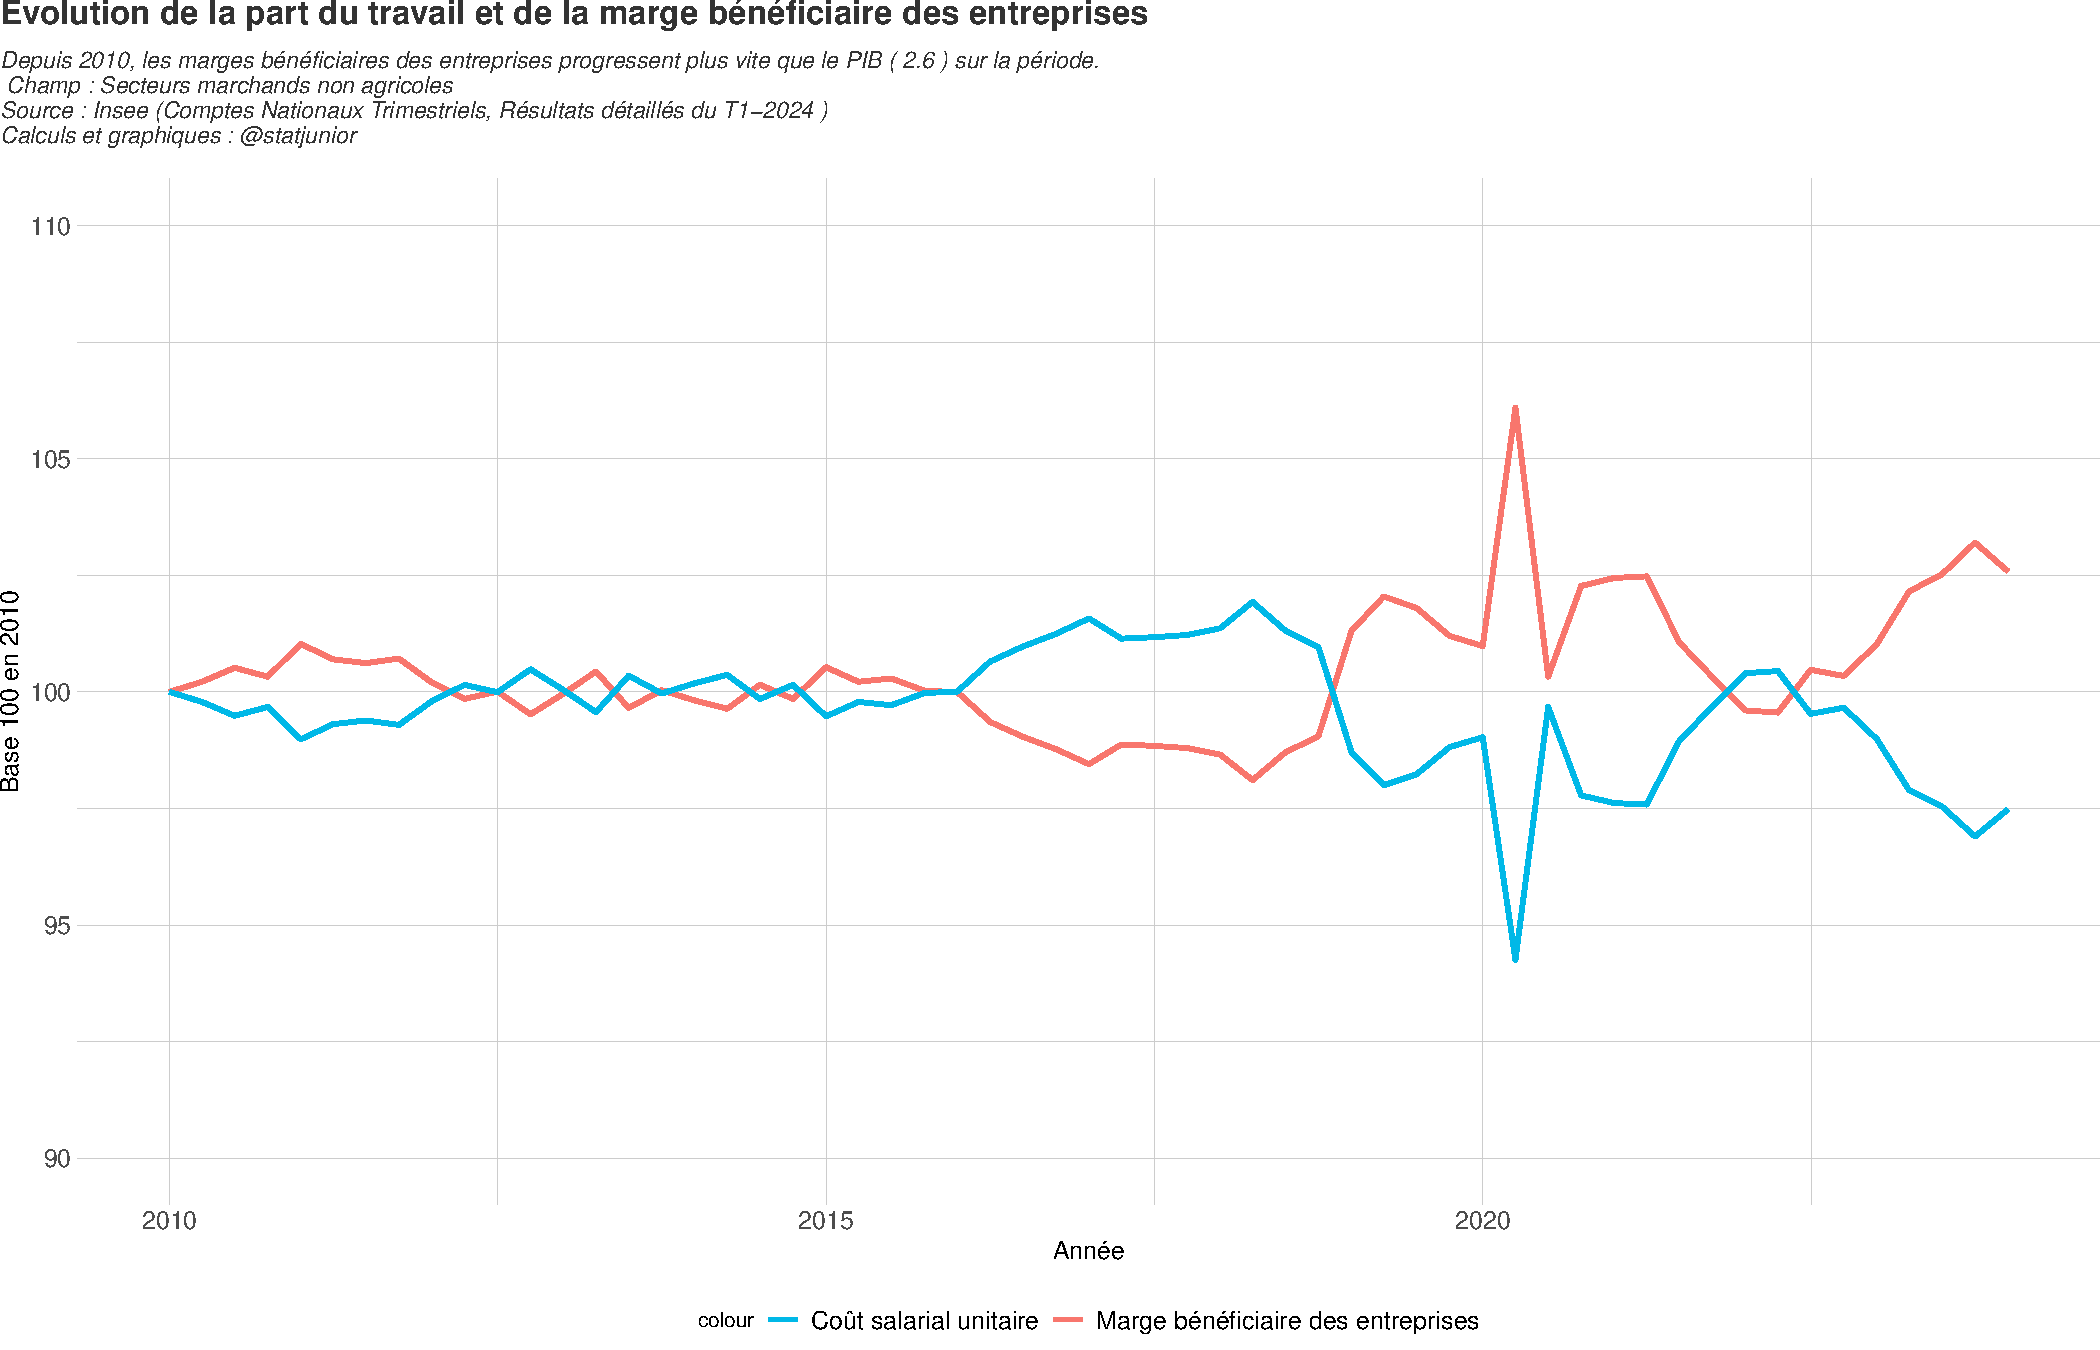
\includegraphics[keepaspectratio]{rapport_pdf_compte_branche_files/figure-latex/unnamed-chunk-43-1.pdf}}

\subsection{Evolution du coût salarial unitaire et du Salaire Moyen par
Tête depuis
2010}\label{evolution-du-couxfbt-salarial-unitaire-et-du-salaire-moyen-par-tuxeate-depuis-2010}

\pandocbounded{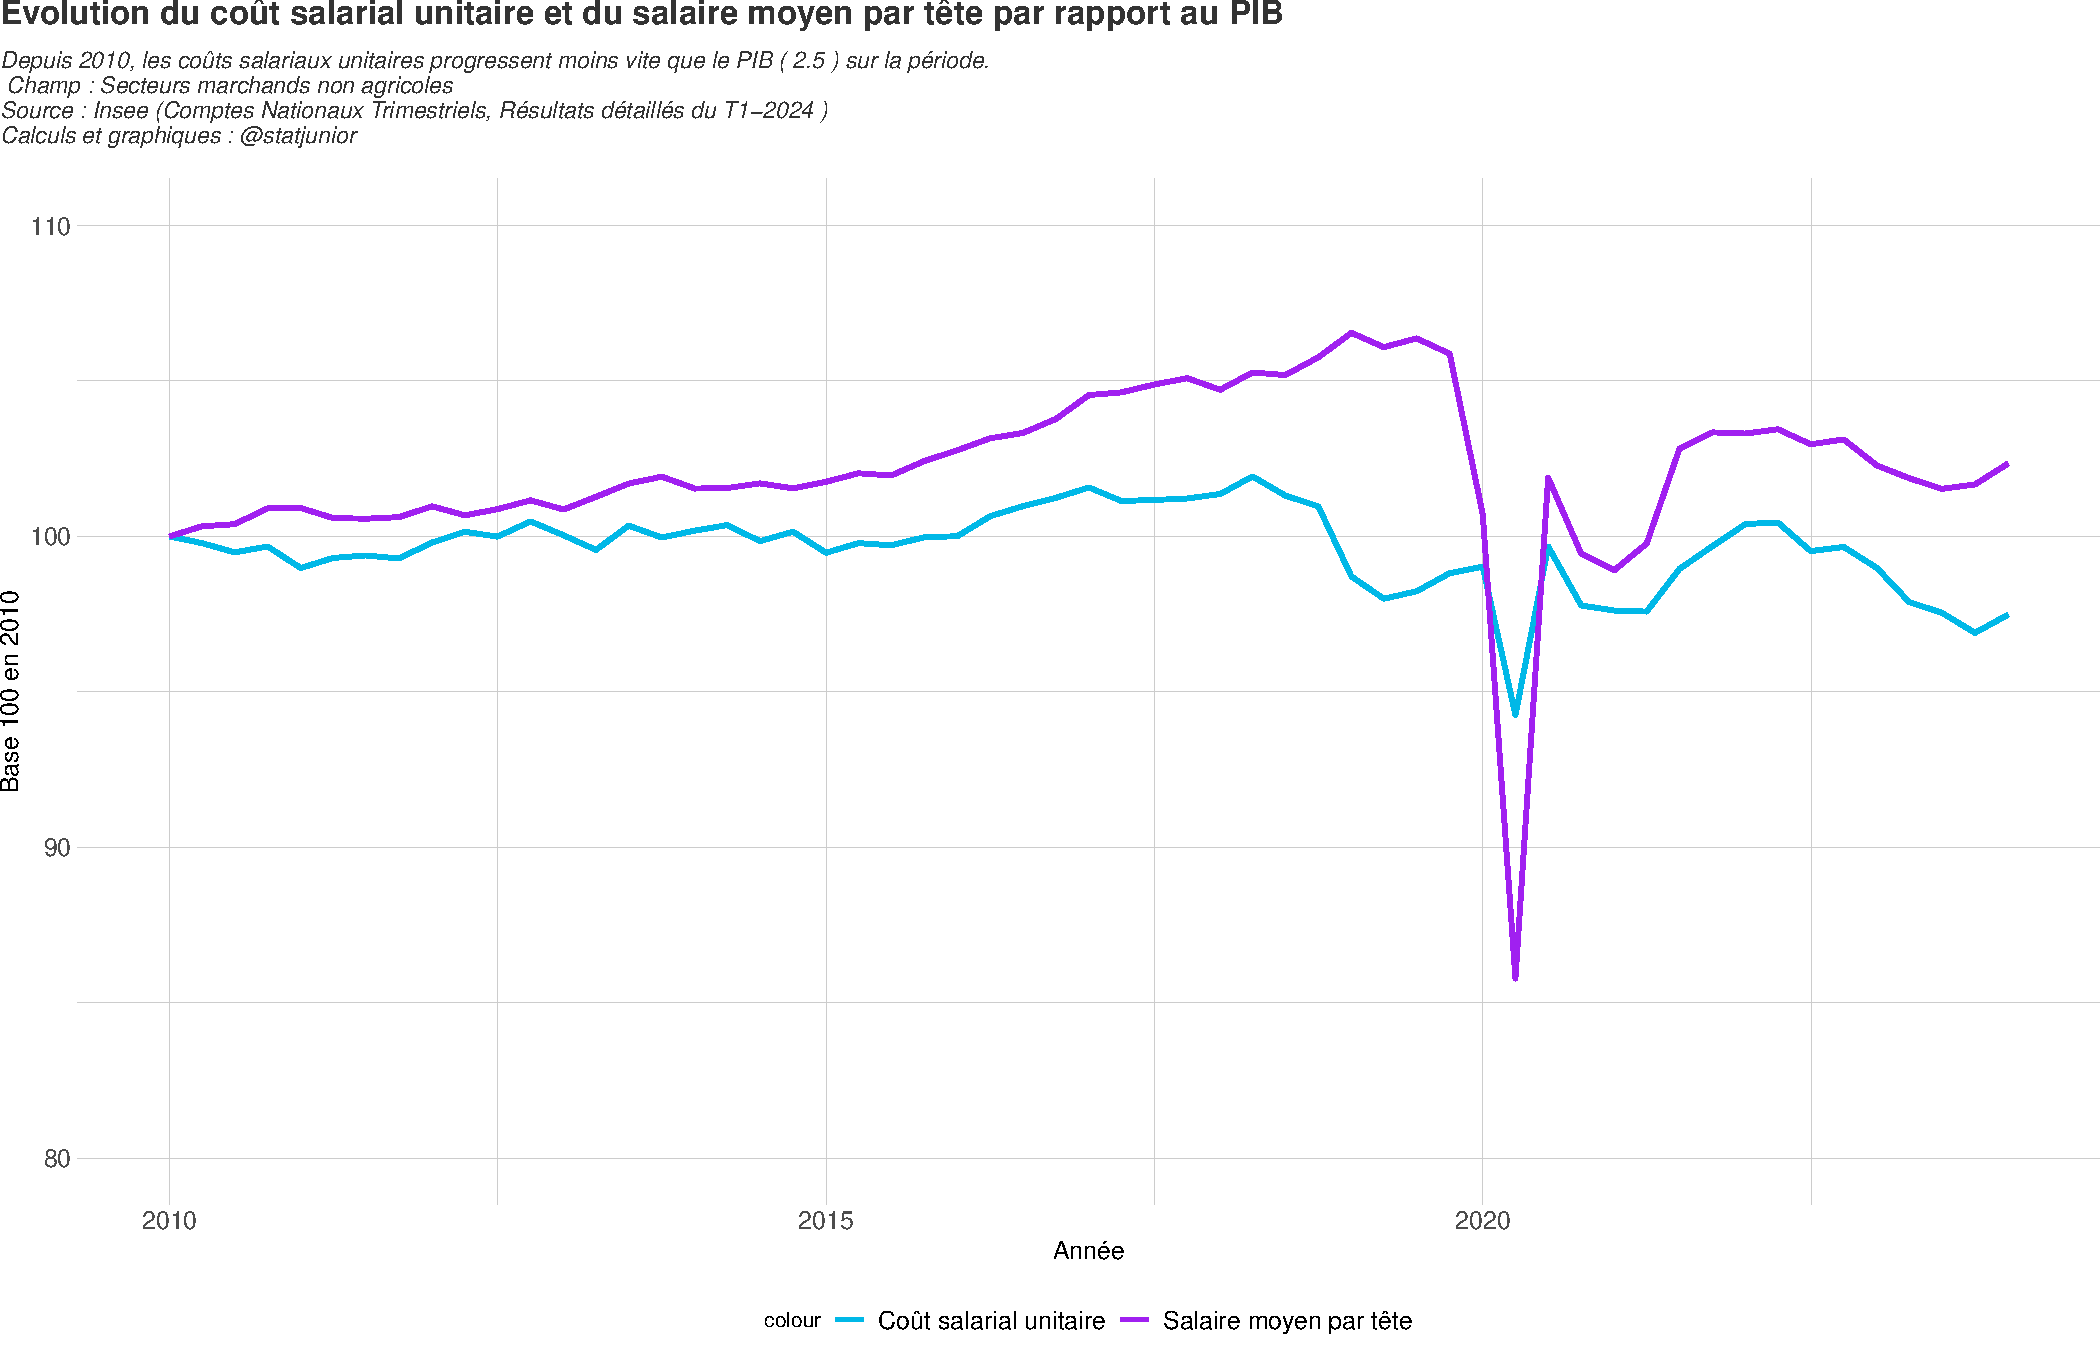
\includegraphics[keepaspectratio]{rapport_pdf_compte_branche_files/figure-latex/unnamed-chunk-44-1.pdf}}

\subsection{Contribution des marges unitaires et des coûts salariaux
unitaires à l'inflation du
PIB}\label{contribution-des-marges-unitaires-et-des-couxfbts-salariaux-unitaires-uxe0-linflation-du-pib}

\pandocbounded{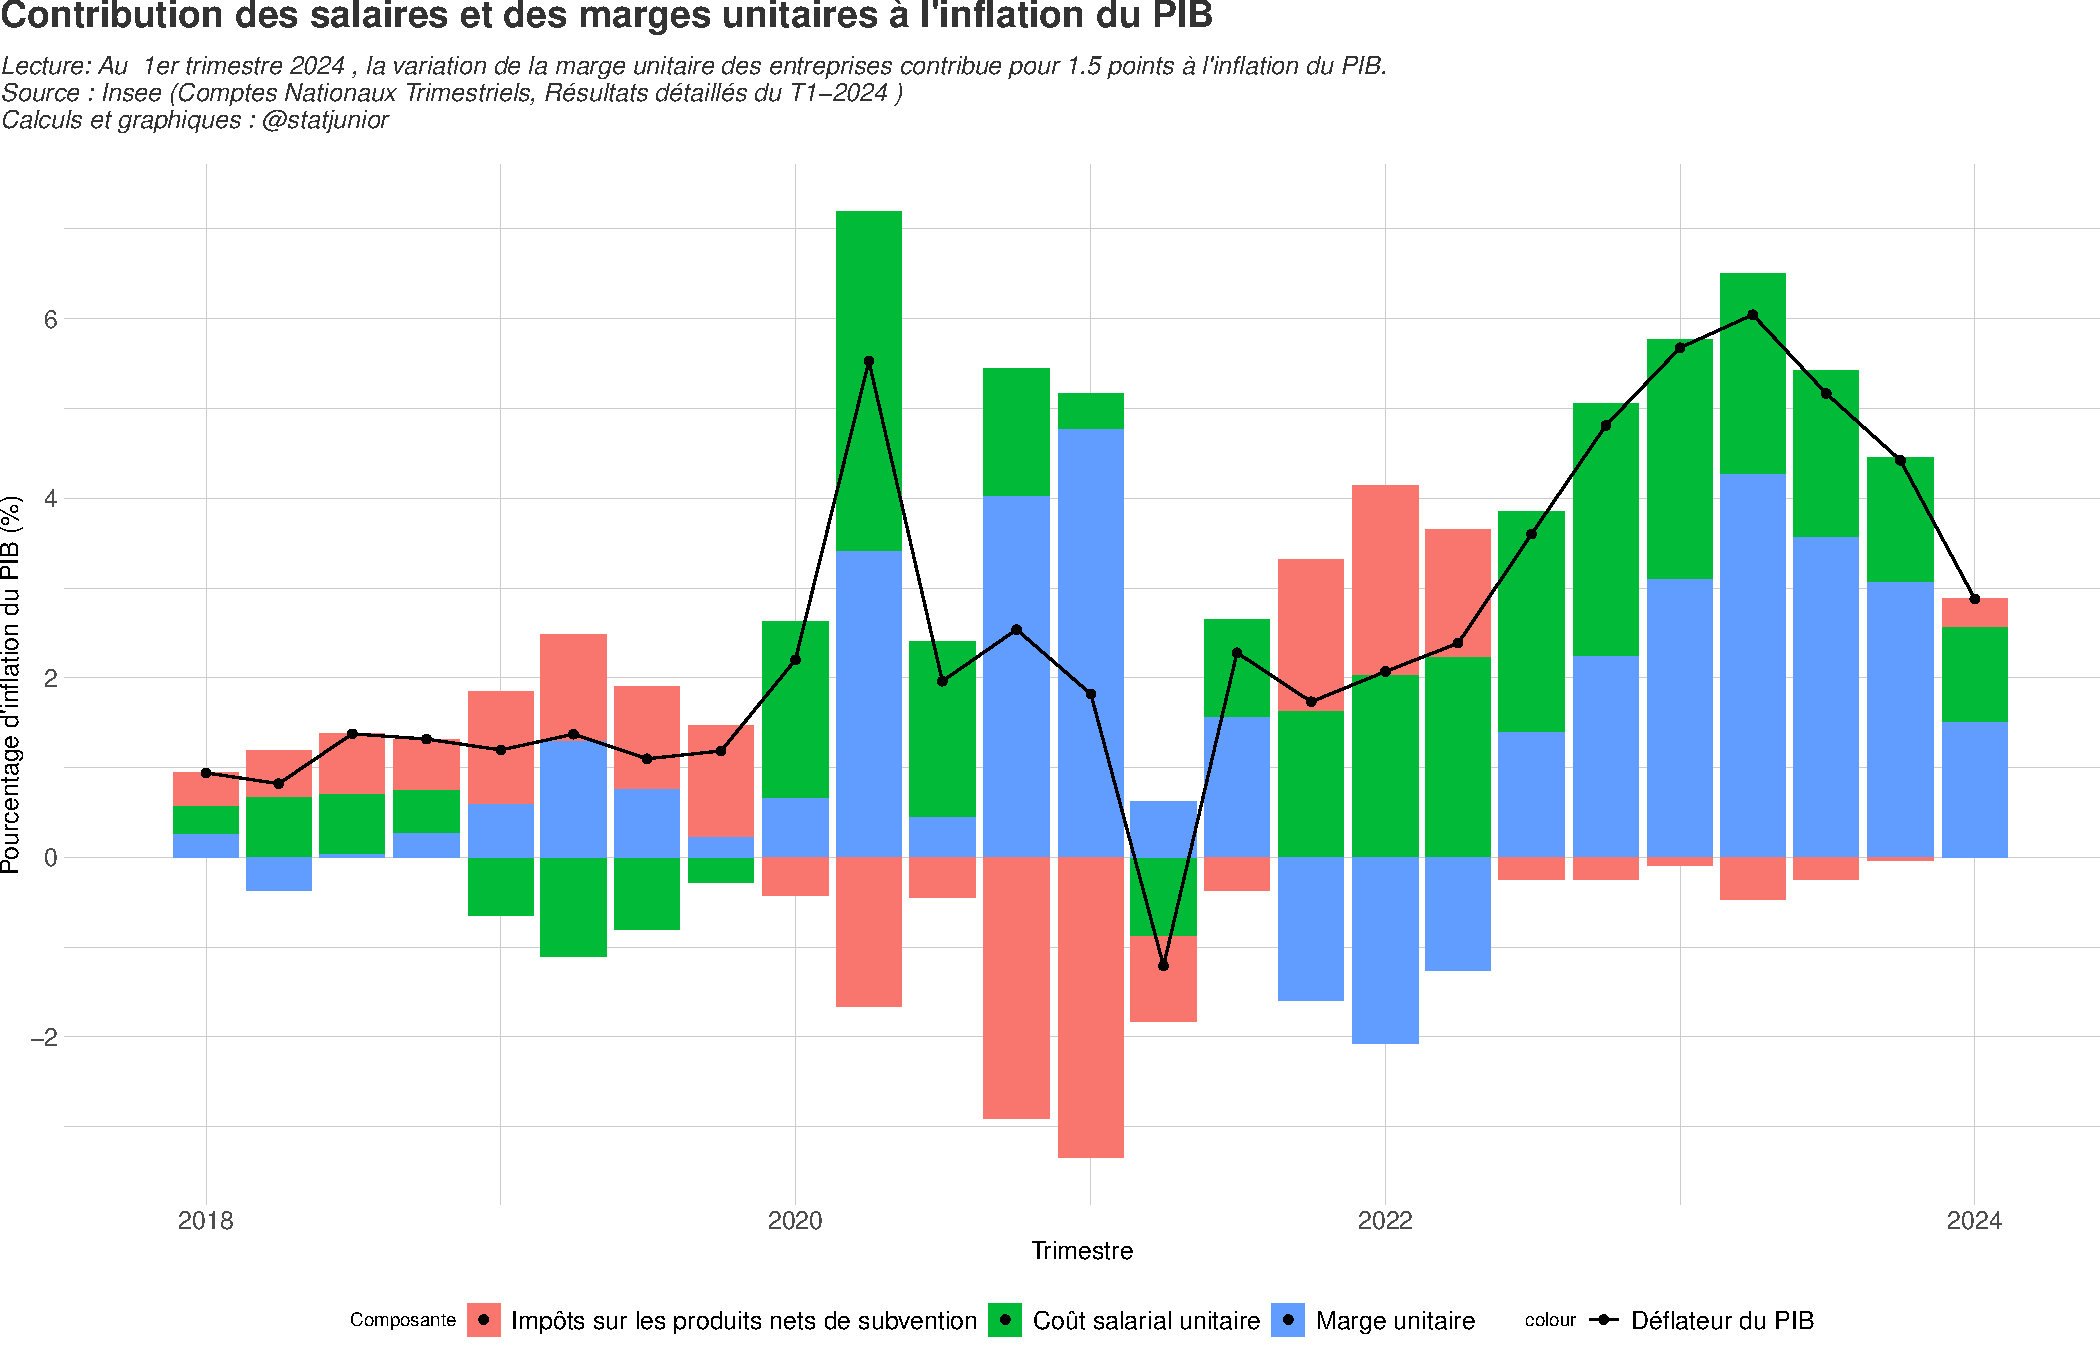
\includegraphics[keepaspectratio]{rapport_pdf_compte_branche_files/figure-latex/unnamed-chunk-47-1.pdf}}

\subsection{Contribution du taux de marge et des coûts salariaux
unitaires à l'inflation du
PIB}\label{contribution-du-taux-de-marge-et-des-couxfbts-salariaux-unitaires-uxe0-linflation-du-pib}

\pandocbounded{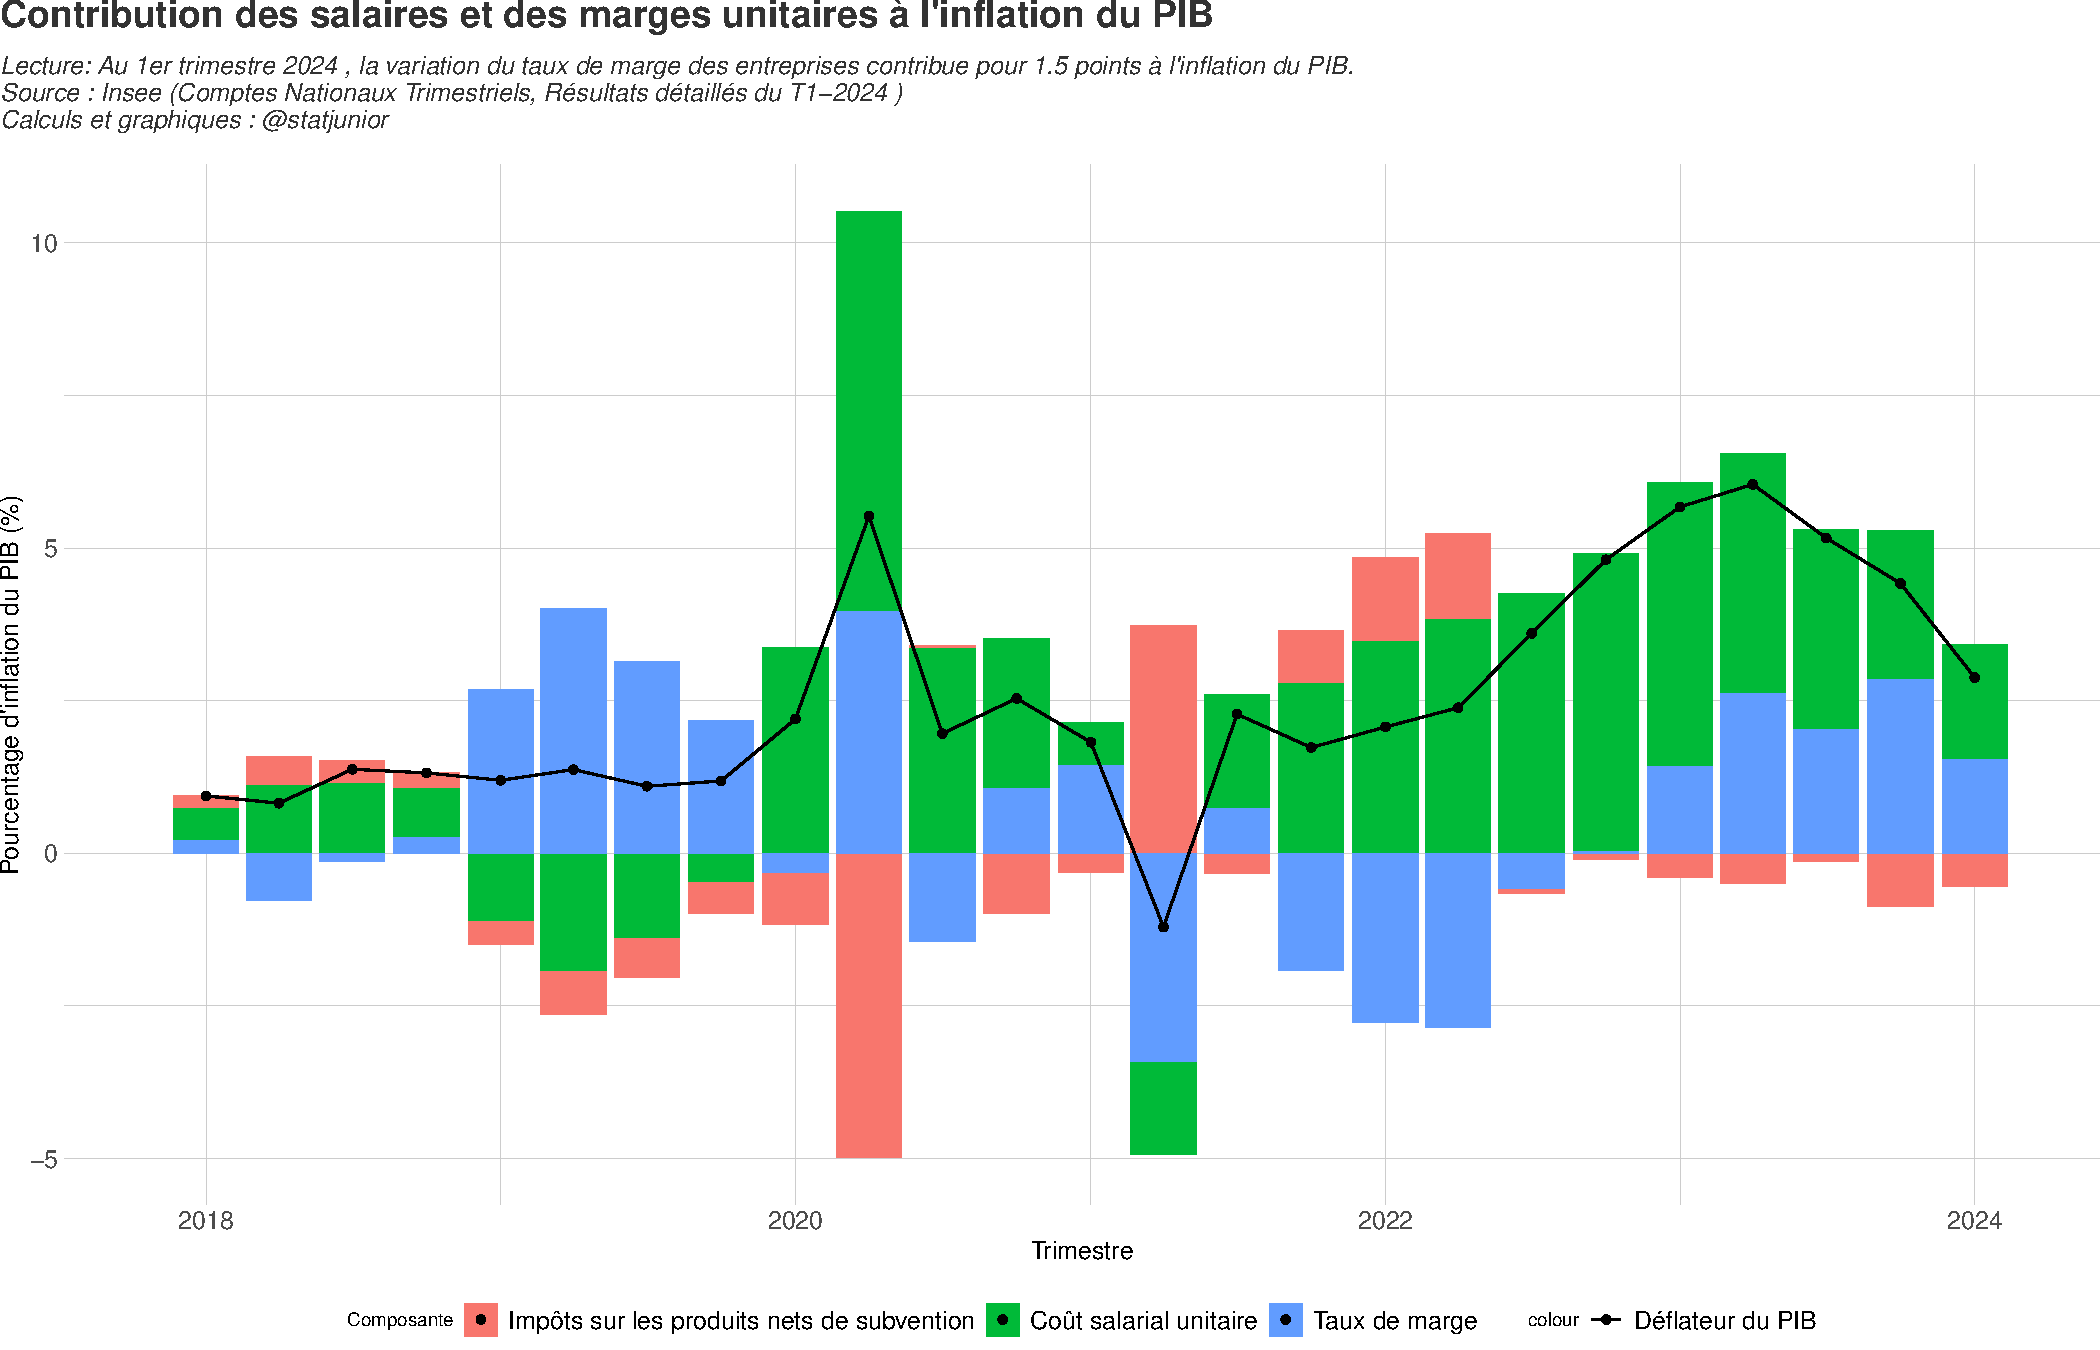
\includegraphics[keepaspectratio]{rapport_pdf_compte_branche_files/figure-latex/unnamed-chunk-49-1.pdf}}

\end{document}
